\documentclass[12pt,a4paper]{report}
\renewcommand{\baselinestretch}{2.0}
\usepackage{longtable}
\usepackage[T1]{fontenc}
\usepackage{times,newtxmath,newtxtext}
\usepackage[utf8]{inputenc}
\usepackage{subcaption}
\usepackage{setspace}
\usepackage{multirow}
\usepackage{multicol}
\usepackage[tableposition=top]{caption}
\usepackage[table,xcdraw]{xcolor}
\usepackage{titlesec}
\usepackage{indentfirst}
\usepackage{enumitem}
\usepackage{overpic}
\usepackage{tikz}
\usepackage{booktabs}
\usepackage{amsmath}
\usepackage{siunitx}
\usepackage{chemformula}


\setlength{\parindent}{1cm}

\captionsetup[table]{labelsep=space}
\captionsetup[figure]{labelsep=space}

\usetikzlibrary{shapes.geometric, arrows, positioning, fit}
\definecolor{blu}{RGB}{135,206,250}
\definecolor{ore}{RGB}{255,140,0}
\tikzstyle{process} = [rectangle, rounded corners, minimum width=4cm, minimum height=1cm, text centered, text width=5cm, draw=black, fill=blu]
\tikzstyle{process2} = [rectangle, rounded corners, minimum width=3cm, minimum height=1cm, text centered, text width=3cm, draw=black, fill=blu]
\tikzstyle{decision} = [diamond, minimum width=2.2cm, minimum height=0.3cm, text centered, text width=1.1cm, draw=black, fill=orange!40]
\tikzstyle{arrow} = [thick,->,>=stealth]

\usepackage{gensymb}
\usepackage{notoccite}
\usepackage{float}
\usepackage{hyperref}
\hypersetup{
    colorlinks,
    citecolor=black,
    filecolor=black,
    linkcolor=black,
    urlcolor=black,
    linkbordercolor=red
}
\usepackage{indentfirst}
\usepackage{amsmath}

\title{Rancang Bangun Instrumentasi Sensor \textit{Tunneling Magnetoresistance} Berbasis Nanofiber \ch{Fe3O4}/PVA-Sitrat-ADH untuk Deteksi Formalin pada Bakso Menggunakan Komparasi Model Klasik (SVM, Random Forest) dan Kuantum (QSVC, VQC)}
\author{Fahry Rizky Samsudin}
\date{September 2026}

\renewcommand{\chaptername}{BAB }
\renewcommand{\figurename}{Gambar}
\renewcommand{\tablename}{Tabel}
\renewcommand{\contentsname}{DAFTAR ISI}
\renewcommand{\listtablename}{DAFTAR TABEL}
\renewcommand{\listfigurename}{DAFTAR GAMBAR}
\renewcommand{\bibname}{DAFTAR PUSTAKA}

\renewcommand{\thechapter}{\Roman{chapter}}
\renewcommand{\thesection}{\arabic{chapter}.\arabic{section}.}
\renewcommand{\thesubsection}{\arabic{chapter}.\arabic{section}.\arabic{subsection}.}
\renewcommand{\thesubsubsection}{\arabic{chapter}.\arabic{section}.\arabic{subsection}.\arabic{subsubsection}.}

\renewcommand{\thefigure}{\arabic{chapter}.\arabic{figure}.}
\renewcommand{\thetable}{\arabic{chapter}.\arabic{table}.}
\renewcommand{\theequation}{\arabic{chapter}.\arabic{equation}}

\usepackage{graphicx}
\graphicspath{{Gambar/}{Gambar/Bab1/}{Gambar/Bab2/}{Gambar/Bab3/}{Gambar/Lampiran/}{Gambar/Logo/}}
\usepackage[a4paper,top=40mm,bottom=30mm,left=40mm,right=30mm]{geometry}

\usepackage{tocloft}
\renewcommand{\cfttoctitlefont}{\hspace*{\fill}\Large\bfseries}
\renewcommand{\cftaftertoctitle}{\hspace*{\fill}}
\renewcommand{\cftlottitlefont}{\hspace*{\fill}\Large\bfseries}
\renewcommand{\cftafterlottitle}{\hspace*{\fill}}
\renewcommand{\cftloftitlefont}{\hspace*{\fill}\Large\bfseries}
\renewcommand{\cftafterloftitle}{\hspace*{\fill}}
\renewcommand{\cftchapleader}{\cftdotfill{\cftchapdotsep}}
\renewcommand{\cftchapdotsep}{\cftdotsep}

\usepackage{sectsty}

\chapternumberfont{\Large} 
\chaptertitlefont{\Large}
\pagenumbering{roman}
\sectionfont{\normalsize}
\subsectionfont{\normalsize}
\titleformat{\section}{\large\bfseries}{\thesection}{1em}{}
\titlespacing\section{0pt}{12pt plus 4pt minus 2pt}{0pt plus 2pt minus 2pt}
\titlespacing\subsection{0pt}{12pt plus 4pt minus 2pt}{0pt plus 2pt minus 2pt}
\titlespacing\subsubsection{0pt}{12pt plus 4pt minus 2pt}{0pt plus 2pt minus 2pt}

\titleformat{\chapter}[display]
	{\normalfont\large\bfseries\centering}{\chaptertitlename \thechapter \centering}{-10pt}{\large}
\titlespacing*{\chapter}{0pt}{-30pt}{20pt}

\setcounter{secnumdepth}{4}
\setcounter{tocdepth}{4}

\usepackage{listings}
\usepackage{xcolor}
\definecolor{codegreen}{rgb}{0,0.6,0}
\definecolor{codegray}{rgb}{0.5,0.5,0.5}
\definecolor{codepurple}{rgb}{0.58,0,0.82}
\definecolor{backcolour}{rgb}{1,1,1}

\lstdefinestyle{mystyle}{
    backgroundcolor=\color{backcolour},   
    commentstyle=\color{codegreen},
    keywordstyle=\color{magenta},
    numberstyle=\tiny\color{codegray},
    stringstyle=\color{codepurple},
    basicstyle=\ttfamily\footnotesize,
    breakatwhitespace=false,         
    breaklines=true,                 
    captionpos=b,                    
    keepspaces=true,                 
    numbers=left,                    
    numbersep=5pt,                  
    showspaces=false,                
    showstringspaces=false,
    showtabs=false,                  
    tabsize=2
}

\lstset{style=mystyle}


\begin{document}
\newgeometry{a4paper,top=4cm,bottom=3cm,left=4cm,right=3cm}

\begin{titlepage}
\thispagestyle{empty}
    \begin{center}
        \begin{spacing}{1.15}
        \textbf{\large RANCANG BANGUN INSTRUMENTASI SENSOR \textit{TUNNELING MAGNETORESISTANCE} BERBASIS NANOFIBER \ch{Fe3O4}/PVA-SITRAT-ADH UNTUK DETEKSI FORMALIN PADA BAKSO MENGGUNAKAN KOMPARASI MODEL KLASIK (SVM, RANDOM FOREST) DAN KUANTUM (QSVC, VQC)}
        \end{spacing}
                
        \vfill
        \textbf{\large PROPOSAL TUGAS AKHIR}
        
        \vspace{0.4cm}
        \begin{spacing}{1.1}
        \textbf{Diajukan Sebagai Salah Satu Syarat Melaksanakan Penelitian Tugas Akhir \\ Jurusan Fisika Fakultas Sains dan Teknologi \\ Universitas Islam Negeri Sunan Gunung Djati Bandung}
        \end{spacing}

        \vfill
        
\includegraphics[width=4.2cm]{Logo UIN.png}

        \vfill
        \begin{spacing}{1.1}
        \textbf{\underline{Fahry Rizky Samsudin}\\
        1237030018}
        \end{spacing}
        
        \vfill
        \begin{spacing}{1.15}
        \textbf{JURUSAN FISIKA\\
        FAKULTAS SAINS DAN TEKNOLOGI\\
        UNIVERSITAS ISLAM NEGERI SUNAN GUNUNG DJATI BANDUNG\\
        \vspace{0.3cm}
        \large 2026}
        \end{spacing}
    \end{center}
\end{titlepage}
\newpage

\setstretch{2}
\chapter*{\centering SURAT PERNYATAAN KEASLIAN}
\addcontentsline{toc}{chapter}{SURAT PERNYATAAN KEASLIAN}

\setstretch{1.15}
\thispagestyle{plain}

Saya yang bertanda tangan di bawah ini:

\begin{center}
\begin{tabular}{ p{3.2cm} p{0.3cm} p{9cm} }
Nama & : & Fahry Rizky Samsudin \\
NIM & : & 1237030018 \\
Jurusan & : & Fisika \\
\end{tabular}
\end{center}

Dengan ini saya menyatakan sebagai berikut:

\begin{enumerate}[noitemsep, topsep=2pt, parsep=2pt, leftmargin=*]
    \item Proposal Tugas Akhir berjudul \textbf{“Rancang Bangun Instrumentasi Sensor \textit{Tunneling Magnetoresistance} Berbasis Nanofiber \ch{Fe3O4}/PVA-Sitrat-ADH untuk Deteksi Formalin pada Bakso Menggunakan Komparasi Model Klasik (SVM, Random Forest) dan Kuantum (QSVC, VQC)}” ini merupakan hasil karya pribadi.
    \item Karya tulis ini sepenuhnya merupakan hasil pemikiran, perumusan, dan penelitian saya sendiri, dengan pengecualian berupa arahan dari dosen, diskusi bersama rekan, serta masukan dari pembimbing.
    \item Segala isi karya tulis ini bukan merupakan karya atau pendapat orang lain yang telah dipublikasikan, kecuali yang telah disertai dengan keterangan sumber secara jelas.
\end{enumerate}

\vspace{0.4cm}
\begin{flushright}
Bandung, 23 September \the\year{} \\  
Yang membuat pernyataan, \\[1.3cm]  
\textbf{Fahry Rizky Samsudin} \\  
NIM. 1237030018  
\end{flushright}
\newpage

\chapter*{\centering LEMBAR PERSETUJUAN}
\addcontentsline{toc}{chapter}{LEMBAR PERSETUJUAN}

\setstretch{1.5}
\thispagestyle{plain}

\begin{center}

Proposal Skripsi\\
\textbf{“Rancang Bangun Instrumentasi Sensor \textit{Tunneling Magnetoresistance} Berbasis Nanofiber \ch{Fe3O4}/PVA-Sitrat-ADH untuk Deteksi Formalin pada Bakso Menggunakan Komparasi Model Klasik (SVM, Random Forest) dan Kuantum (QSVC, VQC)}”\\

\vspace{1cm}
\textbf{FAHRY RIZKY SAMSUDIN\\
1237030018}


\vspace{1cm}
\textbf{Disetujui dan Disahkan} \\
Pada ... \the\year{} \\
Calon Pembimbing, \\
\vspace{2.5cm}
\underline{ \textbf{Mada Sanjaya W.S., M.Si., Ph.D.} } \\
NIP. 19851101 200912 1005 \\

\vspace{1cm}

\textbf{Mengetahui,} \\
Ketua Jurusan Fisika \\
Fakultas Sains dan Teknologi \\
Universitas Islam Negeri Sunan Gunung Djati Bandung \\
\vspace{2.5cm}
\underline{ \textbf{Mada Sanjaya W.S., M.Si., Ph.D.} } \\
NIP. 19851101 200912 1005 \\
\end{center}
%\chapter*{\centering LEMBAR PENGESAHAN}
\addcontentsline{toc}{chapter}{LEMBAR PENGESAHAN}

\setstretch{1.5}
\thispagestyle{empty}

Laporan Kerja Mandiri Terpantau dengan judul : \textbf{“Perancangan Kit Eksperimen Otomatisasi untuk Hukum Pergeseran Wien Berbasis Sensor RGB TCS34725, Arduino Uno R3, dan Antarmuka Python 3”} milik Gilang Pratama Putra Siswanto dengan NIM 1227030017 telah dipertanggungjawabkan dalam sidang Kerja Mandiri Terpantau (KMT) Jurusan Fisika Fakultas Sains dan Teknologi UIN Sunan Gunung Djati Bandung pada tanggal 19 September 2025, persetujuan:


\vspace{1cm}

\begin{center}

\textbf{Mengesahkan}, \\
Penguji Sidang \\
\vspace{2.75cm}
\underline{ \textbf{Ridwan Ramdani, S.Si., M.Si.} } \\
NIP. 19890416 201903 1016 \\

\vspace{1cm}

\textbf{Mengetahui}, \\
Ketua Jurusan Fisika \\
\vspace{2.75cm}
\underline{ \textbf{Mada Sanjaya WS, M.Si., Ph.D} } \\
NIP. 19851011 200912 1005 \\
\end{center}
%\chapter*{\centering ABSTRAK}
\addcontentsline{toc}{chapter}{ABSTRAK}

\begin{center}
\setstretch{1.2}
\begin{tabular}{l l}
Nama          & : Gilang Pratama Putra Siswanto \\ 
Program Studi & : Fisika \\ 
Judul         & : \begin{tabular}[c]{@{}l@{}}Perancangan Kit Eksperimen Otomatisasi untuk \\ Hukum Pergeseran Wien Berbasis Sensor RGB \\ TCS34725, Arduino Uno R3, dan Antarmuka Python 3\end{tabular} \\ 
\end{tabular}
\end{center}

\vspace{1cm}

\begin{spacing}{1.25}
\noindent Penelitian ini bertujuan untuk menganalisis akurasi dan ketelitian kit eksperimen Hukum Pergeseran Wien berbasis Arduino Uno dan sensor TCS34725 dalam mengukur hubungan antara suhu dan panjang gelombang radiasi benda hitam. Dengan mengadopsi teknologi modern, eksperimen ini dilakukan di Laboratorium Instrumentasi-Robotika Universitas Islam Negeri Sunan Gunung Djati pada bulan September-Oktober 2024. Metodologi penelitian meliputi penggunaan sensor suhu dan sensor spektrum yang terintegrasi dengan mikrokontroler untuk menentukan panjang gelombang maksimum yang dipancarkan oleh benda pada suhu tertentu. Hasil pengujian menunjukkan bahwa sistem digital yang dikembangkan dapat bekerja secara optimal dan akurat, menghasilkan nilai konstanta pergeseran Wien (b) sebesar 0,002897773 dengan ketelitian 1,8796E-09 dan ketepatan 99,99\% terhadap nilai literatur. Penelitian ini diharapkan memberikan pemahaman lebih mendalam tentang aplikasi otomatisasi dalam eksperimen fisika serta kontribusinya terhadap pengembangan ilmu pengetahuan. \\

\noindent\textbf{Kata kunci:} Hukum Pergeseran Wien, Arduino Uno, sensor TCS34725, pengukuran suhu, radiasi benda hitam.
\end{spacing}

%\chapter*{\centering ABSTRACT}
\addcontentsline{toc}{chapter}{ABSTRACT}

\begin{center}
\setstretch{1.2}
\begin{tabular}{l l}
Name          & : Gilang Pratama Putra Siswanto \\ 
Study Program & : Physics \\ 
Title         & : \begin{tabular}[c]{@{}l@{}}Design of an Automation Experiment Kit \\for Wien’s Displacement Law Based on TCS34725 \\ RGB Sensor, Arduino Uno R3, and Python 3 Interface\end{tabular} \\ 
\end{tabular}
\end{center}

\vspace{1cm}

\begin{spacing}{1.25}
\noindent This research aims to analyze the accuracy and precision of the Wien Displacement Law experimental kit based on Arduino Uno and the TCS34725 sensor in measuring the relationship between temperature and the wavelength of black body radiation. By adopting modern technology, this experiment was conducted at the Instrumentation and Robotics Laboratory of the State Islamic University of Sunan Gunung Djati from September to October 2024. The research methodology involves the use of temperature sensors and spectrum sensors integrated with a microcontroller to determine the maximum wavelength emitted by an object at a certain temperature. The testing results indicate that the developed digital system operates optimally and accurately, producing a Wien displacement constant (b) value of 0.002897773 with a precision of 1,8796E-09 and an accuracy of 99.99\% compared to the literature value. This research is expected to provide a deeper understanding of the application of automation in physics experiments and its contribution to the development of science. \\

\noindent\textbf{Keywords:} Wien Displacement Law, Arduino Uno, TCS34725 sensor, temperature measurement, black body radiation.
\end{spacing}

\chapter*{\centering KATA PENGANTAR}
\addcontentsline{toc}{chapter}{KATA PENGANTAR}

\setstretch{1.15}  % Mengurangi spasi dalam bagian ini saja
\setlength{\parskip}{0.3em} % Mengatur jarak antar paragraf

Puji syukur selalu terpanjat kehadirat Allah SWT atas segala rahmat, petunjuk, dan kesempatan yang diberikan sehingga penulis dapat menyelesaikan proposal tugas akhir dengan judul ``Rancang Bangun Instrumentasi Sensor \textit{Tunneling Magnetoresistance} Berbasis Nanofiber \ch{Fe3O4}/PVA-Sitrat-ADH untuk Deteksi Formalin pada Bakso Menggunakan Komparasi Model Klasik (SVM, Random Forest) dan Kuantum (QSVC, VQC)''.

Penulis menghaturkan terima kasih dan apresiasi kepada seluruh pihak yang telah berkontribusi positif terhadap penulis. Ucapan terima kasih penulis haturkan kepada:

\begin{enumerate}[noitemsep, topsep=2pt, parsep=0pt, partopsep=0pt]
    \item Allah Subhanahu Wa Ta'ala, karena atas nikmat, karunia, dan izin-Nya lah, Alhamdulillah proposal tugas akhir ini selesai disusun.
    \item Ibu Ara Kusmirah serta segenap keluarga yang tidak henti memberikan dukungan secara moril dan material.
    \item Bapak Mada Sanjaya W.S., M.Si., Ph.D., selaku Dosen Pembimbing Tugas Akhir yang senantiasa memberikan ilmu, arahan, bimbingan, hingga motivasi selama proses penelitian dan penulisan proposal tugas akhir ini.
    \item Segenap civitas akademika Fisika UIN SGD Bandung yang telah menyisihkan waktunya dalam memberikan pengetahuan, diskursus, dan motivasi yang berarti bagi penulis, khususnya dalam mempelajari keilmuan dalam menyelesaikan proposal tugas akhir.
    \item Alma Triana Nabilla, yang tidak henti membersamai, memberikan dukungan penuh secara moril dan material setiap waktunya, sehingga penulis memiliki motivasi tinggi dalam menyelesaikan studi strata I. Semoga hal-hal baik senantiasa beriring secara simultan di antara ruang dan waktu padanya.
    % TODO(Fahry): tambahkan di sini pihak lain yang ingin diucapkan terima kasih
    % (dosen pembimbing akademik, rekan penelitian/lab, sahabat, dsb.) sesuai
    % dengan orang-orang yang sebenarnya terlibat dalam proses studimu.
\end{enumerate}

Dengan penuh kerendahan hati, penulis menyadari bahwa proposal ini turut jauh dari kata sempurna dan memiliki banyak keterbatasan. Karenanya, penulis sangat mengharapkan kritik serta saran yang membangun. Semoga proposal ini dapat memberikan manfaat bagi penulis pribadi, maupun bagi pengembangan ilmu pengetahuan, teknologi, serta pihak-pihak yang memerlukannya.

\vspace{0.2cm}
\begin{flushright}
    Bandung, 23 September \the\year{}\\[1.2cm]
    \textbf{Fahry Rizky Samsudin}
\end{flushright}

\chapter*{\centerline{DAFTAR ISI}}
\addcontentsline{toc}{chapter}{DAFTAR ISI}

% Pengaturan spasi daftar isi
\renewcommand{\baselinestretch}{1} 
\normalsize

\makeatletter
\@starttoc{toc}
\makeatother

% Kembalikan ke spasi normal setelah daftar isi
\renewcommand{\baselinestretch}{1.5}
\normalsize

\newpage

\chapter*{\centerline{DAFTAR GAMBAR}}
\addcontentsline{toc}{chapter}{DAFTAR GAMBAR}

\makeatletter
\@starttoc{lof}
\makeatother

\newpage
\chapter*{\centerline{DAFTAR TABEL}}
\addcontentsline{toc}{chapter}{DAFTAR TABEL}

\makeatletter
\@starttoc{lot}
\makeatother

\newpage

\chapter{PENDAHULUAN}
\pagenumbering{arabic}

\section{Latar Belakang}

Formalin (larutan formaldehida) merupakan bahan kimia berbahaya yang dilarang keras penggunaannya sebagai bahan tambahan pangan di Indonesia berdasarkan Peraturan Menteri Kesehatan Republik Indonesia No. 033/2012. Kendati demikian, praktik penyalahgunaannya sebagai pengawet ilegal masih kerap ditemukan pada produk pangan olahan hewani siap saji, salah satunya bakso \cite{menlhk_formalin,padang_bakso,sosis_efsa}. Berbagai studi identifikasi di lapangan secara konsisten melaporkan temuan positif formalin pada sampel bakso yang beredar di pasar tradisional maupun pedagang kaki lima, seperti di Kota Padang \cite{padang_bakso}, sepanjang Jalan Soebrantas Kota Pekanbaru \cite{pekanbaru_bakso}, hingga di area wisata dan kantin sekolah di Yogyakarta \cite{yogyakarta_bakso}. Salah satu penelitian di Pekanbaru bahkan melaporkan kadar formalin pada sampel bakso mencapai 4,506~ppm \cite{pekanbaru_bakso}, padahal Otoritas Keamanan Pangan Eropa (\textit{European Food Safety Authority}/EFSA) menetapkan ambang batas toleransi residu formalin dalam pangan maksimal hanya sebesar 100~ppm \cite{sosis_efsa}. Mengingat formaldehida bersifat karsinogenik golongan 1 (IARC), paparan residu secara berulang meskipun dalam konsentrasi rendah berpotensi terakumulasi dalam jaringan biologis dan memicu kerusakan organ kronis. Kondisi tersebut menegaskan urgensi tersedianya sistem deteksi formalin yang objektif, memiliki sensitivitas tinggi untuk menjangkau ambang batas regulasi pangan, serta mampu memberikan konfirmasi kuantitatif secara langsung di lapangan.

Metode pengujian formalin konvensional saat ini masih didominasi oleh uji kualitatif menggunakan reagen warna kimia (seperti kalium permanganat $\mathrm{KMnO_4}$, pereaksi asam kromotropat, maupun \textit{rapid test kit} komersial) serta metode analitik laboratorium berbasis spektrofotometri UV-Vis dan kromatografi cair kinerja tinggi (HPLC). Meskipun metode laboratorium memiliki akurasi tinggi dan batas deteksi (\textit{limit of detection}/LOD) di bawah 1~mg/L, metode tersebut bersifat destruktif terhadap sampel, memerlukan prosedur derivatisasi kimiawi yang kompleks dan memakan waktu (30--60 menit per sampel), melibatkan reagen kimia toksik (seperti pereaksi Nash atau 2,4-DNPH), serta menggunakan instrumen stasioner yang mahal sehingga tidak fleksibel untuk inspeksi lapangan. Sebaliknya, metode uji cepat kolorimetri di lapangan umumnya hanya menghasilkan indikasi visual biner (ada atau tidaknya perubahan warna) dengan batas deteksi yang relatif kasar (10--50~mg/L), serta sangat rentan terhadap bias interpretasi subjektif dari operator. Kesenjangan antara metode laboratorium yang akurat tetapi lambat dan uji cepat visual yang rentan galat mendorong intensifnya riset pengembangan sensor analitik berbasis elektronik.

Dalam perkembangannya, berbagai sensor elektronik dan biosensor telah dieksplorasi untuk mendeteksi formalin, di antaranya sensor gas berbasis semikonduktor oksida logam (\textit{metal oxide semiconductor}/MOS), biosensor elektrokimia berbasis enzim, dan sensor kolorimetri digital terintegrasi optoelektronik. Sensor gas MOS berbasis $\mathrm{SnO_2}$ atau $\mathrm{In_2O_3}$ bekerja melalui perubahan konduktivitas permukaan akibat desorpsi oksigen saat bereaksi dengan gas formaldehida, menghasilkan batas deteksi pada rentang sub-ppm (0.05--1.0~ppm) \cite{wang2021mos}. Namun, sensor MOS menuntut suhu operasional tinggi (200--400~$^\circ\mathrm{C}$) yang membutuhkan pemanas berdaya besar sehingga tidak ramah baterai portabel, serta memiliki kelemahan mendasar berupa interferensi silang (\textit{cross-sensitivity}) terhadap kelembapan udara dan senyawa volatil bumbu bakso (seperti uap alkohol dan asam asetat). Di sisi lain, biosensor elektrokimia memanfaatkan enzim \textit{formaldehyde dehydrogenase} (FDH) yang menawarkan selektivitas biokimiawi tinggi dengan LOD hingga 0.02~mg/L \cite{singhal2024food}. Kendati demikian, enzim merupakan makromolekul yang sangat labil dengan masa simpan pendek (kurang dari 3 minggu), memerlukan kofaktor $\mathrm{NAD}^+$ yang mahal, sangat sensitif terhadap perubahan suhu dan pH lingkungan, serta rentan mengalami peracunan elektroda (\textit{electrode fouling}) akibat adsorpsi makromolekul lemak dan protein bakso pada permukaan sensor. Sementara itu, sistem sensor optoelektronik dan kolorimetri digital yang mengandalkan analisis warna citra digital \cite{sun2023optical} sangat rentan terdistorsi oleh kekeruhan alami (\textit{turbidity}) dan pigmen alami daging bakso, sehingga tetap membutuhkan preparasi sentrifugasi bertingkat. Keterbatasan-keterbatasan tersebut memicu kebutuhan akan platform sensor alternatif yang mampu beroperasi stabil pada suhu ruang, hemat energi, kebal terhadap warna atau kekeruhan sampel fisik, dan memiliki reseptor sintetis berkestabilan tinggi, yang salah satu solusinya bermuara pada biosensor magnetoresistif berbasis nanokomposit magnetik.

Pemanfaatan nanokomposit magnetik berbasis serat nano (\textit{nanofiber}) menjadi pendekatan inovatif dalam merealisasikan elemen pengenal (\textit{chemo-receptor}) yang selektif dan berdaya tahan tinggi. Nanopartikel \ch{Fe3O4} memiliki keunggulan berupa sifat superparamagnetik, suseptibilitas magnetik tinggi, dan biokompatibilitas yang sangat baik \cite{antarnusa2022,ardiyanti2025}. Melalui teknik elektrospinning, matriks polimer polivinil alkohol (PVA) yang terdispersi nanopartikel \ch{Fe3O4} dapat dibentuk menjadi jejaring nanofiber berpori dengan rasio luas permukaan terhadap volume yang masif \cite{xue2019electrospinning,Turkoglu2024}, sehingga menyediakan densitas situs aktif interaksi analit yang berlimpah. Pada arsitektur nanokomposit ini, asam sitrat berperan ganda sebagai agen penstabil dispersi (\textit{capping agent}) nanopartikel \ch{Fe3O4} sekaligus agen penaut silang hijau (\textit{green crosslinker}) tunggal bagi rantai polimer PVA. Melalui reaksi esterifikasi termal (\textit{thermal curing}) pada suhu $130\,^{\circ}\mathrm{C}$, asam sitrat membentuk jejaring ester kovalen antar-rantai PVA yang memperkokoh integritas mekanik serta ketahanan air (\textit{water resistance}) membran tanpa melepaskan residu toksik \cite{shi2008citric,birck2014citric}. Sementara itu, fungsi pengenalan analit dipercayakan secara khusus kepada \textit{adipic acid dihydrazide} (ADH) yang difungsionalisasikan sebagai reseptor kimiawi (\textit{chemo-receptor}). Berbeda dari glutaraldehida (GA) yang tergolong dialdehida dan rentan memicu reaksi silang kompetitif serta ambiguitas pengenalan analit, ADH memiliki dua gugus terminal hidrazida (\ch{-NH-NH2}) yang bereaksi secara spontan, spesifik, dan kovalen dengan gugus karbonil formaldehida membentuk ikatan hidrazon (\ch{-C=N-NH-}) yang stabil pada suhu ruang \cite{sigma_adh,gantrade_adh}. Pemisahan peran fungsional yang tegas ini---asam sitrat sebagai penaut silang struktural dan ADH sebagai reseptor molekuler---menjamin stabilitas fisik membran sekaligus spesifisitas pengenalan formaldehida yang tinggi.

Interaksi spesifik antara molekul formaldehida dan gugus hidrazida ADH pada permukaan nanofiber memodulasi momen magnetik lokal serta sebaran medan magnetik bocor (\textit{stray field}) dari nanopartikel \ch{Fe3O4}. Deteksi pergeseran sinyal medan magnetik mikro tersebut menuntut transduser magnetik dengan resolusi dan sensitivitas tinggi. Sebagian besar penelitian biosensor magnetik terdahulu memanfaatkan sensor \textit{Giant Magnetoresistance} (GMR) dengan rasio magnetoresistansi $\Delta R/R$ berkisar 10--15\% dan sensitivitas rasiometrik 2--4~mV/V/mT \cite{gilang2026skripsi}. Guna meningkatkan batas resolusi deteksi, penelitian ini menerapkan transduser \textit{Tunneling Magnetoresistance} (TMR) komersial tipe ALT023-10E. Sensor TMR beroperasi berdasarkan fenomena penerobosan terowongan kuantum (\textit{quantum tunneling effect}) melintasi lapisan penghalang isolator magnesium oksida (MgO) berorde nanometer pada struktur \textit{magnetic tunnel junction} (MTJ) \cite{nanomedicine_mtj}. Mekanisme \textit{tunneling} ini menghasilkan rasio magnetoresistansi melampaui 200\% pada suhu ruang serta sensitivitas diferensial 15--25~mV/V/mT, yakni berlipat ganda dibandingkan sensor GMR pada rentang medan magnet rendah $\pm 1.0$~mT \cite{nve_alt023}. Karakteristik sensitivitas tersebut memungkinkan transduser TMR menangkap pergeseran fluks magnetik lokal akibat interaksi formalin pada konsentrasi rendah secara presisi.

Pembacaan sinyal diferensial sensor TMR yang berada pada orde fraksi milivolt membutuhkan rantai instrumentasi presisi tinggi sebelum dikonversi menjadi data digital. Pada penelitian ini, keluaran diferensial sensor TMR dikuatkan menggunakan \textit{instrumentation amplifier} AD623 bertegangan tunggal $+5.0\text{ V}$ dengan tegangan referensi presisi $V_{\text{REF}} = 2.50\text{ V}$ yang dibentuk melalui pembagi tegangan resistor presisi $1.0\text{ k}\Omega$ \cite{adi_ad623}. Rangkaian diperkuat dengan tapis lolos-rendah aktif (\textit{active RC low-pass filter}) berfrekuensi potong $f_c = 10\text{ Hz}$ guna meredam ripple jala-jala listrik 50~Hz serta derau termal lingkungan. Sinyal analog yang telah tersaring didigitasi oleh ADC eksternal ADS1115 16-bit beresolusi tinggi (0.1875~mV/count) \cite{ti_ads1115}, diakuisisi mikrokontroler Arduino Uno secara deterministik berbasis interupsi, dan ditransmisikan secara serial ke modul pemroses utama. Kepastian validitas dan keterulangan (\textit{repeatability}) metrologis dijamin melalui kalibrasi awal sistem menggunakan medan magnet acuan terkontrol dari sepasang kumparan Helmholtz terstandardisasi dan teslameter terkalibrasi \cite{zhu2023,ginisa2015,yudhistira2019}.

Tantangan berikutnya terletak pada karakteristik respons sinyal biosensor terhadap konsentrasi formalin pada matriks pangan nyata (bakso), yang kerap menunjukkan perilaku nonlinearitas, histeresis mikro, dan fluktuasi akibat derau matriks biologis (kandungan garam, lemak, dan protein daging). Mengandalkan regresi linear sederhana semata rentan menimbulkan galat estimasi konsentrasi yang signifikan. Oleh karena itu, diterapkan pemodelan cerdas berbasis ekstraksi tiga fitur sinyal domain waktu utama: tegangan rata-rata kondisi tunak ($V_{\text{mean}}$), pergeseran tegangan respons terhadap baseline ($\Delta V$), dan simpangan baku fluktuasi derau sinyal ($\sigma_V$). Vektor fitur tiga dimensi ($d=3$) ini memberikan representasi kompak yang ideal untuk dipetakan secara terukur ke dalam tiga qubit ($n=3$) pada ruang keadaan Hilbert kuantum berdimensi $2^3 = 8$. Pemodelan dilakukan melalui komparasi komprehensif antara dua paradigma: dua model klasik, yaitu \textit{Support Vector Machine} (SVM) dan \textit{Random Forest} (RF), serta dua model kuantum, yaitu \textit{Quantum Support Vector Classifier} (QSVC) dan \textit{Variational Quantum Classifier} (VQC). Pada paradigma klasik, SVM dengan kernel \textit{Radial Basis Function} (RBF) memetakan batas keputusan nonlinear berdasarkan prinsip \textit{structural risk minimization} \cite{cortes1995support}, sementara Random Forest memanfaatkan agregasi pohon keputusan (\textit{ensemble bagging}) yang tangguh terhadap variansi data sensor \cite{Breiman2001,Tyralis2019}. Pada paradigma kuantum (\textit{Quantum Machine Learning}/QML), QSVC menghitung matriks kemiripan data menggunakan \textit{Quantum Kernel Estimator} berbasis sirkuit penyandian $ZZ\text{FeatureMap}$ \cite{havlicek2019supervised,schuld2019quantum}, sedangkan VQC melatih gerbang rotasi kuantum parametrik (\textit{parameterized quantum circuit}) secara variasional melalui penurunan gradien \cite{schuld2019quantum}. Evaluasi komparatif keempat model menggunakan validasi silang \textit{5-fold cross validation} dengan metrik akurasi, presisi, \textit{recall}, \textit{F1-score}, efisiensi komputasi, dan ketahanan derau (\textit{noise resilience}) menjadi kontribusi analitis penting dalam mengevaluasi potensi komputasi kuantum pada instrumentasi analitik pangan.

Berdasarkan keseluruhan landasan pemikiran di atas, hingga saat ini belum ditemukan penelitian yang secara terpadu mengintegrasikan transduser sensor \textit{Tunneling Magnetoresistance} (TMR) beresolusi tinggi, material fungsional nanofiber \ch{Fe3O4}/PVA-Sitrat-ADH sebagai elemen reseptor kovalen selektif, rantai instrumentasi akuisisi analog-digital AD623-ADS1115 yang stabil, serta komparasi model klasifikasi cerdas dua model klasik (SVM dan RF) versus dua model kuantum (QSVC dan VQC) untuk deteksi formalin pada bakso. Oleh sebab itu, penelitian ini dirancang untuk menjawab tantangan tersebut secara komprehensif, mulai dari fabrikasi material, perancangan mekatronika perangkat keras, kalibrasi metrologis, pengujian analit formalin pada sampel bakso riil, hingga analisis komparasi performa model komputasi cerdas. Hasil penelitian ini diharapkan dapat menjadi fondasi ilmiah yang kokoh dalam melahirkan instrumen biosensor formalin yang portabel, berakurasi tinggi, dan terjangkau guna mendukung penjaminan keamanan pangan nasional.



\section{Rumusan Masalah}
Berdasarkan latar belakang di atas maka permasalahan yang dapat dirumuskan adalah sebagai berikut:
\begin{enumerate}
    \item Bagaimana sensitivitas, batas deteksi (\textit{limit of detection}/LOD), dan pengaruh gugus fungsional hidrazida ADH terhadap karakteristik respons magnetoresistif sensor TMR berbasis nanofiber \ch{Fe3O4}/PVA-Sitrat-ADH dalam mendeteksi variasi konsentrasi formalin?
    \item Bagaimana karakteristik medan magnetik acuan kumparan Helmholtz dan respons linearitas transduser TMR ALT023-10E sebelum dan sesudah integrasi rantai pengkondisi sinyal?
    \item Bagaimana rancangan sistem instrumentasi (AD623-ADS1115-Arduino-Raspberry Pi) menghasilkan kurva kalibrasi yang valid antara tegangan keluaran sensor dan konsentrasi formalin pada bakso?
    \item Bagaimana komparasi performa klasifikasi antara model klasik (\textit{Support Vector Machine} dan \textit{Random Forest}) serta model kuantum (\textit{Quantum Support Vector Classifier} dan \textit{Variational Quantum Classifier}) dalam mendeteksi dan mengklasifikasikan kandungan formalin pada sampel bakso?
\end{enumerate}


\section{Batasan Masalah}
Batasan masalah dalam penelitian ini ditetapkan agar fokus pengujian tetap terarah dan terukur, meliputi:
\begin{enumerate}
    \item Penelitian ini difokuskan khusus pada deteksi analit formalin; bahan tambahan pangan berbahaya lain seperti boraks atau pewarna tekstil tidak termasuk cakupan analisis.
    \item Pengujian sensor diawali menggunakan larutan formalin standar hasil pengenceran bertingkat dengan konsentrasi terkontrol (mg/L) sebagai dasar kurva kalibrasi, sebelum diterapkan pada ekstrak sampel bakso riil.
    \item Material sensor yang digunakan adalah nanofiber \ch{Fe3O4}/PVA-Sitrat-ADH hasil elektrospinning dengan penautan silang termal asam sitrat dan fungsionalisasi gugus reseptor hidrazida ADH.
    \item Mekanisme pengenalan formalin oleh gugus hidrazida ADH pada penelitian ini diperlakukan sebagai hipotesis yang diuji secara empiris melalui respons transduksi magneto-mekanik, bukan mekanisme yang telah dibuktikan secara pasti.
    \item Evaluasi sensor TMR dibatasi pada parameter sensitivitas, linearitas, batas deteksi (LOD), dan kestabilan sinyal; aspek lain seperti ketahanan mekanik jangka panjang tidak menjadi fokus utama.
    \item Pemodelan cerdas dibatasi pada perbandingan dua paradigma: dua model klasik (\textit{Support Vector Machine} ber-kernel RBF dan \textit{Random Forest}) serta dua model kuantum (\textit{Quantum Support Vector Classifier} berbasis $ZZ\text{FeatureMap}$ dan \textit{Variational Quantum Classifier} berbasis sirkuit kuantum parametrik) yang disimulasikan menggunakan pustaka Qiskit pada komputer klasik.
\end{enumerate}


\section{Tujuan Penelitian}
Berdasarkan rumusan masalah di atas, penelitian ini bertujuan untuk:
\begin{enumerate}
    \item Mengevaluasi sensitivitas, batas deteksi (LOD), serta pengaruh fungsionalisasi gugus fungsional hidrazida ADH terhadap karakteristik respons magnetoresistif sensor TMR berbasis nanofiber \ch{Fe3O4}/PVA-Sitrat-ADH dalam mendeteksi variasi konsentrasi formalin.
    \item Mengkarakterisasi medan magnetik acuan kumparan Helmholtz serta respons linearitas transduser TMR ALT023-10E sebelum dan sesudah integrasi rantai pengkondisi sinyal.
    \item Merancang dan memvalidasi sistem instrumentasi akuisisi data (AD623-ADS1115-Arduino-Raspberry Pi) yang menghasilkan kurva kalibrasi valid antara tegangan keluaran sensor dan konsentrasi formalin pada bakso.
    \item Menganalisis dan membandingkan performa klasifikasi (akurasi, presisi, \textit{recall}, \textit{F1-score}, efisiensi komputasi, dan ketahanan derau) antara model klasik (SVM dan RF) serta model kuantum (QSVC dan VQC) dalam mengklasifikasikan kandungan formalin pada sampel bakso.
\end{enumerate}

\section{Manfaat Penelitian}
Penelitian ini akan memberikan beberapa manfaat, di antaranya:
\begin{enumerate}
    \item Memberikan kontribusi teoretis dalam pengembangan ilmu instrumentasi sensor dengan menghadirkan kajian mengenai performa sensor \textit{Tunneling Magnetoresistance} (TMR) berbasis nanofiber \ch{Fe3O4}/PVA-Sitrat-ADH untuk deteksi formalin.
    \item Menawarkan pendekatan baru melalui pemisahan peran fungsional material: asam sitrat sebagai agen penaut silang hijau (\textit{green crosslinker}) ramah lingkungan yang mengeliminasi glutaraldehida toksik, dan \textit{adipic acid dihydrazide} (ADH) sebagai reseptor kovalen spesifik yang selektif mengenali gugus karbonil formaldehida melalui formasi ikatan hidrazon.
    \item Memberikan kontribusi kebaruan ilmiah dalam penerapan komparasi komputasi kuantum (\textit{Quantum Machine Learning}: QSVC dan VQC) terhadap model klasik (SVM dan RF) untuk klasifikasi sinyal sensor pada pengujian keamanan pangan.
    \item Menjadi dasar bagi pengembangan instrumen deteksi formalin yang cerdas, portabel, kuantitatif, dan terjangkau untuk mendukung pengawasan keamanan pangan nasional.
\end{enumerate}

\section{Metode Pengumpulan Data}
Pencapaian tujuan penelitian ditempuh melalui serangkaian metode pengumpulan data sebagai berikut:
\begin{enumerate}
    \item Studi Literatur: Mengumpulkan dan menganalisis informasi dari penelitian terdahulu mengenai deteksi formalin pada pangan, teknologi \textit{Tunneling Magnetoresistance} (TMR), material nanofiber \ch{Fe3O4}/PVA-Sitrat-ADH, serta algoritma pemodelan klasik (SVM dan RF) dan kuantum (QSVC dan VQC).
    \item Observasi dan Studi Pendahuluan: Melakukan observasi terhadap prototipe instrumentasi sensor magnetoresistif yang telah dikembangkan sebelumnya, sebagai titik tolak perancangan rangkaian instrumentasi sensor TMR pada penelitian ini, termasuk teknik fabrikasi nanofiber melalui elektrospinning dengan stabilisasi asam sitrat dan fungsionalisasi ADH.
    \item Eksperimen Laboratorium: Merancang dan menguji instrumen sensor TMR berbasis nanofiber \ch{Fe3O4}/PVA-Sitrat-ADH untuk mendeteksi variasi konsentrasi formalin, diawali karakterisasi medan magnet kumparan Helmholtz hingga pengujian sampel bakso riil.
    \item Analisis Data dan Pemodelan Cerdas: Data hasil eksperimen diolah melalui analisis regresi kalibrasi, ekstraksi fitur sinyal ($V_{\text{mean}}$, $\Delta V$, $\sigma_V$), serta pelatihan dan evaluasi komparatif model klasik (SVM, RF) versus model kuantum (QSVC, VQC).
\end{enumerate}

\newpage
\section{Sistematika Penulisan}
Dalam penulisan penelitian ini, diatur sistematika penulisan dalam tiga bab dengan urutan sebagai berikut:
\\
\\
BAB I: PENDAHULUAN

Bab ini berisi uraian mengenai latar belakang penelitian, perumusan masalah, batasan masalah, tujuan penelitian, manfaat penelitian, serta metode pengumpulan data yang digunakan. Bagian ini menjadi landasan awal untuk menjelaskan pentingnya rancang bangun instrumentasi sensor \textit{Tunneling Magnetoresistance} (TMR) berbasis nanofiber \ch{Fe3O4}/PVA-Sitrat-ADH dengan komparasi model klasik (SVM, RF) dan model kuantum (QSVC, VQC) dalam deteksi formalin pada bakso.
\\
\\
BAB II: TINJAUAN PUSTAKA

Bab ini membahas kajian pustaka dan teori-teori yang relevan dengan penelitian, meliputi permasalahan formalin pada pangan, prinsip kerja sensor \textit{Tunneling Magnetoresistance} (TMR), dasar material pembentuk nanofiber (PVA, Asam Sitrat, ADH, dan nanofiber komposit), komponen instrumentasi perangkat keras, hingga dasar teori pemodelan komparasi model klasik (SVM, RF) dan model kuantum (QSVC, VQC).
\\
\\
BAB III: METODE PENELITIAN DAN PERANCANGAN SISTEM

Bab ini memuat daftar alat dan bahan yang digunakan, tahapan sintesis terstruktur nanofiber komposit melalui elektrospinning dengan parameter optimal, perancangan sistem akuisisi data perangkat keras dan perangkat lunak, serta metodologi ekstraksi fitur dan evaluasi komparatif model klasik (SVM, RF) versus model kuantum (QSVC, VQC).

\chapter{TINJAUAN PUSTAKA}

\section{Dasar Teori}
\subsection{Formaldehida}
\begin{figure}[H]
    \centering
    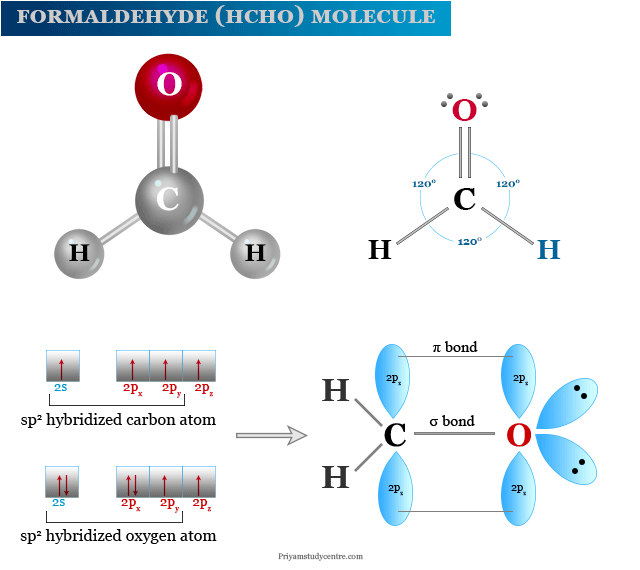
\includegraphics[width=8cm]{babII_ikatan_formalin.png}
    \caption{Struktur Molekul dan Hibridisasi Ikatan Kimia Formaldehida}
    \label{fig:molekul_formaldehida}
\end{figure}

Formaldehida merupakan senyawa aldehida paling sederhana dengan rumus molekul $\mathrm{CH_2O}$, berwujud gas tidak berwarna dengan bau menyengat khas pada suhu ruang, sangat reaktif, dan mudah larut dalam air \cite{halodoc_formalin}. Struktur molekul formaldehida memiliki geometri planar segitiga dengan sudut ikatan mendekati $120^\circ$, di mana atom karbon mengalami hibridisasi $sp^2$ membentuk ikatan $\sigma$ terhadap dua atom hidrogen dan satu atom oksigen, serta satu ikatan $\pi$ pada gugus karbonil ($\mathrm{C=O}$) sebagaimana ditunjukkan pada Gambar~\ref{fig:molekul_formaldehida}. Secara komersial, larutan formaldehida dalam air dengan konsentrasi berkisar 37--40\% berat yang ditambah metanol 10--15\% sebagai stabilisator untuk mencegah polimerisasi formaldehida menjadi paraformaldehida yang mengendap dikenal luas dengan nama dagang formalin \cite{menlhk_formalin}. Secara kimiawi, formaldehida bersifat elektrofilik kuat pada atom karbon karbonilnya, sehingga mudah bereaksi dengan berbagai nukleofil, termasuk gugus amina pada protein, membentuk ikatan silang (\textit{cross-link}) antar-rantai protein. Reaksi inilah yang mendasari kemampuan formalin sebagai bahan pengawet jaringan biologis: ikatan silang protein yang terbentuk membuat jaringan menjadi kaku dan lebih tahan terhadap aktivitas enzim serta mikroorganisme pembusuk \cite{menlhk_formalin}.

Sifat itulah yang disalahgunakan sebagai pengawet pada produk pangan berprotein tinggi seperti bakso, tahu, dan ikan, meskipun formaldehida bersifat toksik dan karsinogenik bagi manusia sehingga penggunaannya pada pangan dilarang secara tegas oleh regulasi kesehatan \cite{halodoc_formalin}. Paparan formaldehida dalam pangan, meskipun dalam kadar kecil namun berulang, berpotensi terakumulasi dan menimbulkan efek toksik kronis. Karakteristik formalin sebagai gugus aldehida reaktif inilah yang menjadi dasar pendekatan deteksi pada penelitian ini, yaitu memanfaatkan reaksi spesifik antara gugus aldehida formaldehida dengan gugus hidrazida pada material reseptor nanofiber (lihat Subbab~\ref{subsec:fe3o4pvaadh}).

\subsection{\textit{Tunneling Magnetoresistance} (TMR)}
\begin{figure}[H]
    \centering
    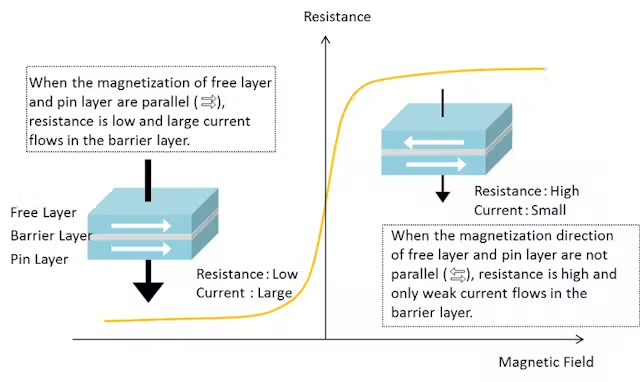
\includegraphics[width=8.5cm]{babII_TMR_Layer.png}
    \caption{Struktur Lapisan \textit{Magnetic Tunnel Junction} (MTJ) pada Sensor \textit{Tunneling Magnetoresistance} (TMR) \cite{nanomedicine_mtj}}
    \label{fig:tmr_layer}
\end{figure}

\textit{Tunneling Magnetoresistance} (TMR) adalah fenomena magnetoresistif yang muncul pada struktur \textit{magnetic tunnel junction} (MTJ), yaitu dua lapisan feromagnetik yang dipisahkan oleh lapisan penghalang (\textit{barrier}) insulator setebal beberapa nanometer, umumnya magnesium oksida (MgO) atau aluminium oksida (Al$_2$O$_3$) \cite{nve_alt023}. Ilustrasi struktur lapisan MTJ pada sensor TMR ditunjukkan pada Gambar~\ref{fig:tmr_layer}. Berbeda dengan GMR yang mengandalkan hamburan elektron terpolarisasi spin pada lapisan logam nonmagnetik konduktif, TMR memanfaatkan efek terowongan kuantum (\textit{quantum tunneling effect}): elektron menembus lapisan penghalang insulator melalui mekanisme tunneling yang probabilitasnya bergantung pada kesejajaran arah momen magnetik kedua lapisan feromagnetik di sekitarnya.

Ketika magnetisasi kedua lapisan feromagnetik paralel, kerapatan keadaan (\textit{density of states}) elektron dengan spin mayoritas pada kedua elektroda saling bersesuaian, sehingga probabilitas tunneling tinggi dan resistansi junction rendah. Sebaliknya, pada kondisi antiparalel, kerapatan keadaan spin mayoritas dan minoritas antar elektroda saling bertukar, sehingga probabilitas tunneling menurun dan resistansi meningkat signifikan. Secara kuantitatif, rasio TMR dirumuskan melalui model Julliere sebagai
\begin{equation}
\mathrm{TMR} = \frac{R_{AP} - R_{P}}{R_{P}} = \frac{2 P_1 P_2}{1 - P_1 P_2},
\label{eq:tmr_julliere}
\end{equation}
dengan $R_{P}$ dan $R_{AP}$ berturut-turut adalah resistansi junction pada kondisi paralel dan antiparalel, sedangkan $P_1$ dan $P_2$ adalah derajat polarisasi spin masing-masing elektroda feromagnetik \cite{nanomedicine_mtj}. Karena efek tunneling jauh lebih sensitif terhadap kesejajaran spin dibandingkan hamburan pada GMR, rasio TMR yang dapat dicapai jauh lebih besar. Sensor berbasis MTJ dengan penghalang MgO dilaporkan mencapai rasio TMR di atas 200\% pada suhu ruang, dibandingkan rasio GMR pada sensor \textit{spin-valve} yang umumnya kurang dari 20\% \cite{nanomedicine_mtj}, dan keluaran sensor TMR komersial dilaporkan dapat mencapai sekitar enam kali lebih tinggi dibandingkan sensor GMR pada aplikasi sejenis \cite{electronicdesign_tmrgmr}.

Sensor TMR analog komersial, seperti seri ALT yang digunakan pada penelitian ini, dikemas dalam konfigurasi jembatan Wheatstone yang tersusun dari elemen-elemen MTJ, menghasilkan keluaran diferensial yang bersifat \textit{bipolar}: bernilai positif untuk medan magnet pada satu arah, dan negatif untuk arah sebaliknya \cite{nve_alt023_evb}. Untuk sensor semacam ini, produsen umumnya menyatakan performa langsung dalam bentuk sensitivitas rasiometrik terhadap tegangan suplai, $\mathrm{Sen}$, dengan satuan mV/V/mT, sehingga tegangan keluaran diferensial dapat dituliskan sebagai
\begin{equation}
V_{out} \approx \mathrm{Sen} \times V_{S} \times B,
\label{eq:tmr_vout}
\end{equation}
dengan $V_S$ tegangan suplai jembatan dan $B$ medan magnet yang terukur pada rentang linear sensor \cite{nve_alt023}. Persamaan \eqref{eq:tmr_vout} berlaku pada rentang medan linear sensor; di luar rentang tersebut sensor mengalami saturasi dan hubungan menjadi tidak linear. Sensitivitas tinggi serta linearitas yang baik pada rentang kerjanya menjadikan sensor TMR unggul untuk aplikasi yang membutuhkan resolusi medan magnet sangat kecil, termasuk deteksi perubahan momen magnetik lokal akibat interaksi analit dengan label/reseptor magnetik pada biosensor maupun sensor kimia \cite{micronas_tmr}.

\subsection{Kumparan Helmholtz}
Kumparan Helmholtz adalah sepasang kumparan melingkar identik dengan radius $R$ dan jumlah lilitan $N$ yang sama, ditempatkan sejajar pada sumbu bersama dan dipisahkan oleh jarak yang sama dengan radiusnya ($\alpha = R$), serta dialiri arus $I$ pada arah yang sama. Konfigurasi ini menghasilkan medan magnet yang relatif homogen pada daerah di sekitar titik tengah antara kedua kumparan, sehingga banyak digunakan untuk kalibrasi sensor magnetik maupun eksperimen fisika yang membutuhkan medan magnet acuan dengan nilai yang diketahui secara akurat \cite{zhu2023,ginisa2015,yudhistira2019}.

Berdasarkan hukum Biot--Savart, medan magnet pada sumbu sebuah kumparan melingkar tunggal berjari-jari $R$ pada jarak $z$ dari pusatnya adalah
\begin{equation}
B_{\text{loop}}(z) = \frac{\mu_0 I R^2}{2 (R^2+z^2)^{3/2}},
\label{eq:helmholtz_loop}
\end{equation}
dengan $\mu_0$ permeabilitas vakum. Untuk kumparan dengan $N$ lilitan, nilai pada Persamaan \eqref{eq:helmholtz_loop} dikalikan $N$. Pada konfigurasi sepasang kumparan Helmholtz yang berjarak $\alpha=R$, medan pada titik tengah ($z=0$) menjadi
\begin{equation}
B(0) = \frac{8}{5\sqrt{5}} \cdot \frac{\mu_0 N I}{R},
\label{eq:helmholtz_center}
\end{equation}
yang merupakan bentuk baku medan Helmholtz di pusat kumparan \cite{zhu2023}. Keunggulan konfigurasi ini terletak pada turunan orde rendah medan terhadap posisi $z$ di sekitar $z=0$ yang bernilai mendekati nol, sehingga daerah dengan medan seragam (\textit{uniform field region}) menjadi relatif luas dibandingkan kumparan tunggal, dan nilai arus $I$ yang diberikan dapat dikonversi langsung menjadi medan magnet $B$ yang diketahui melalui Persamaan \eqref{eq:helmholtz_center}. Sifat inilah yang dimanfaatkan pada tahap karakterisasi sensor TMR dalam penelitian ini, sebagai sumber medan magnet terkendali sebelum dibandingkan dengan pembacaan teslameter sebagai acuan riil.

\subsection{\textit{Instrumentation Amplifier}}
\textit{Instrumentation amplifier} (in-amp) adalah konfigurasi penguat diferensial presisi yang dirancang untuk menguatkan selisih dua sinyal masukan sekaligus menolak sinyal yang muncul bersama pada kedua masukan (\textit{common-mode signal}), seperti derau atau interferensi yang terinduksi pada kedua jalur kabel secara bersamaan \cite{TI2019,Jung2002}. Berbeda dari penguat diferensial op-amp tunggal, in-amp umumnya tersusun dari beberapa tahap op-amp dengan impedansi masukan tinggi, sehingga tidak membebani sumber sinyal, serta memiliki \textit{common-mode rejection ratio} (CMRR) yang jauh lebih tinggi.

Secara umum, keluaran in-amp dapat dituliskan sebagai
\begin{equation}
V_{out} = G \,(V_{+} - V_{-}) + V_{REF},
\label{eq:inamp_out}
\end{equation}
dengan $G$ adalah penguatan (\textit{gain}) yang diatur oleh sebuah resistor eksternal tunggal ($R_G$), dan $V_{REF}$ adalah tegangan referensi keluaran yang dapat digeser untuk mengakomodasi sinyal bipolar pada sistem catu daya tunggal \cite{TI2019}. Untuk in-amp yang mengatur gain melalui satu resistor eksternal (misalnya seri AD62x), hubungan gain terhadap resistor tersebut umumnya berbentuk
\begin{equation}
G = 1 + \frac{R_{gain}}{R_G},
\label{eq:inamp_gain}
\end{equation}
dengan $R_{gain}$ konstanta internal yang nilainya bergantung pada rancangan IC \cite{adi_ad623}. Pemilihan $V_{REF}$ pada nilai tengah rentang catu daya (misalnya setengah dari tegangan suplai) memungkinkan in-amp mengangkat sinyal bipolar kecil ke rentang tegangan positif yang dapat dibaca oleh ADC catu daya tunggal, tanpa memerlukan catu daya negatif \cite{Jung2002}.

\subsection{\textit{Passive Low Pass Filter}}
\begin{figure}[H]
    \centering
    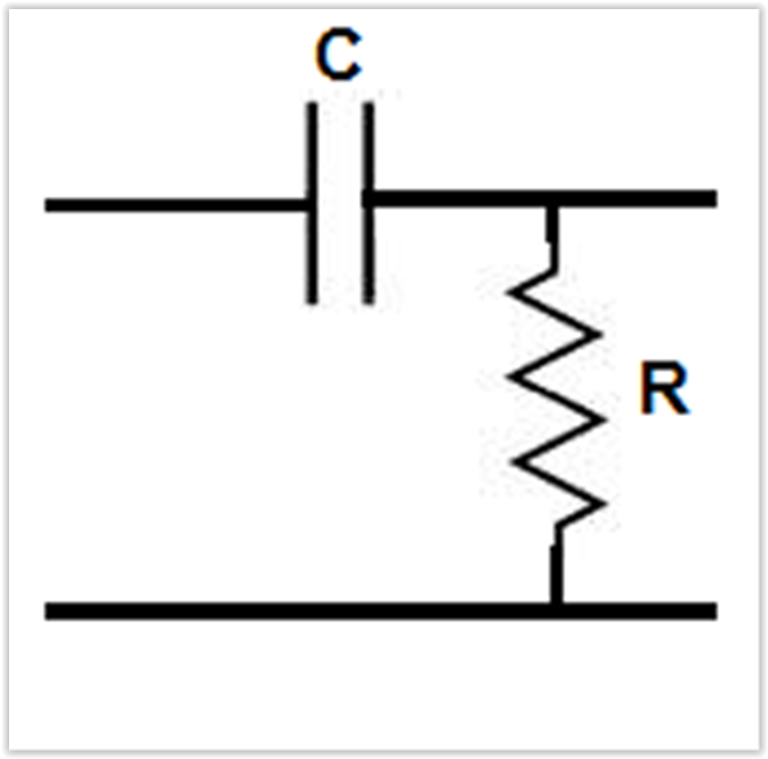
\includegraphics[width=5.5cm]{babII_LPF.PNG}
    \caption{Rangkaian \textit{Passive Low Pass Filter} RC Orde Pertama \cite{Supriyanto2023}}
    \label{fig:lpf_rangkaian}
\end{figure}

\textit{Low pass filter} (LPF) adalah rangkaian elektronik yang melewatkan sinyal berfrekuensi rendah dan melemahkan sinyal berfrekuensi tinggi. Parameter kunci LPF adalah frekuensi cut-off ($f_c$), yaitu frekuensi ketika amplitudo sinyal keluaran turun sebesar 3 dB (sekitar 70,7\%) dari amplitudo maksimum \cite{Firmansyah2017}. Rangkaian dasar \textit{passive low pass filter} RC orde pertama ditunjukkan pada Gambar~\ref{fig:lpf_rangkaian}. LPF pasif orde pertama yang paling sederhana tersusun dari resistor $R$ seri dengan sumber sinyal dan kapasitor $C$ paralel terhadap keluaran. Karena impedansi kapasitor menurun seiring naiknya frekuensi, sinyal frekuensi tinggi cenderung "terhubung singkat" ke ground melalui kapasitor, sementara sinyal frekuensi rendah tetap diteruskan menuju keluaran \cite{Supriyanto2023}. Fungsi transfer rangkaian ini adalah
\begin{equation}
\frac{V_{out}}{V_{in}} = \frac{1}{1+j\omega RC}, \qquad \omega = 2\pi f,
\end{equation}
dengan frekuensi cut-off
\begin{equation}
f_c = \frac{1}{2\pi RC}.
\label{eq:lpf_fc}
\end{equation}
Dalam rangkaian instrumentasi sensor, LPF pasif umumnya ditempatkan pada tahap akhir sebelum ADC sebagai filter \textit{anti-aliasing}, yang berfungsi membatasi bandwidth sinyal analog agar berada di bawah setengah frekuensi \textit{sampling} ADC (kriteria Nyquist), sehingga mencegah distorsi \textit{aliasing} pada hasil konversi digital \cite{Firmansyah2017,Supriyanto2023}.

\subsection{\textit{Analog to Digital Converter} (ADC)}
\textit{Analog to Digital Converter} (ADC) adalah rangkaian yang mengonversi sinyal tegangan analog kontinu menjadi representasi digital diskret. Proses ini melibatkan dua tahap utama: \textit{sampling} (pencuplikan sinyal pada interval waktu tertentu) dan kuantisasi (pemetaan nilai tegangan tercuplik ke tingkat diskret terdekat sesuai resolusi ADC). Kinerja ADC ditentukan oleh resolusi (jumlah bit), laju \textit{sampling}, linearitas, \textit{signal-to-noise ratio} (SNR), dan konsumsi daya \cite{shylu2020power}.

Salah satu arsitektur ADC dengan resolusi tinggi adalah \textit{Delta-Sigma} ($\Delta\Sigma$) ADC, yang bekerja dengan melakukan \textit{oversampling} terhadap sinyal masukan lalu menerapkan \textit{noise shaping} untuk mendorong derau kuantisasi keluar dari pita frekuensi sinyal yang diinginkan, sehingga resolusi efektif tinggi dapat dicapai tanpa memerlukan komponen analog presisi ekstrem \cite{shylu2020power}. Semakin tinggi resolusi ADC (jumlah bit $n$), semakin kecil tegangan minimum yang dapat dibedakan (\textit{least significant bit}, LSB), yang untuk ADC unipolar dengan tegangan rentang penuh $V_{FSR}$ dinyatakan sebagai
\begin{equation}
\mathrm{LSB} = \frac{V_{FSR}}{2^{n}}.
\label{eq:adc_lsb}
\end{equation}
Resolusi tinggi ini menjadi penting pada sistem akuisisi data yang perlu membaca perubahan sinyal sensor berorde milivolt hingga mikrovolt, seperti pada instrumentasi sensor magnetoresistif.

\subsection{\textit{Electrospinning}}
\begin{figure}[H]
    \centering
    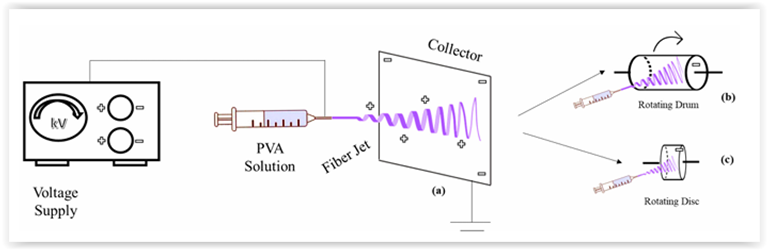
\includegraphics[width=9cm]{babII_elspinPVA.PNG}
    \caption{Ilustrasi Sistem \textit{Electrospinning} untuk Fabrikasi Nanofiber PVA \cite{Turkoglu2024}}
    \label{fig:electrospinning_pva}
\end{figure}

\textit{Electrospinning} merupakan teknik yang memanfaatkan fenomena elektrohidrodinamika untuk menghasilkan serat berukuran nano dari larutan atau lelehan polimer \cite{xue2019electrospinning}. Ilustrasi sistem \textit{electrospinning} untuk pembuatan nanofiber PVA ditunjukkan pada Gambar~\ref{fig:electrospinning_pva}. Sistem \textit{electrospinning} terdiri atas catu daya bertegangan tinggi (DC/AC), pompa \textit{syringe}, \textit{spinneret} (jarum hipodermik berujung tumpul), dan kolektor konduktif. Proses ini berlangsung dalam empat tahap: (i) pembentukan \textit{Taylor cone} akibat gaya tolak elektrostatik yang melampaui tegangan permukaan tetesan larutan; (ii) pemanjangan jet bermuatan searah medan listrik; (iii) penipisan jet yang disertai instabilitas \textit{bending}/\textit{whipping} yang mendominasi pembentukan serat berskala nano; dan (iv) solidifikasi jet akibat penguapan pelarut, menghasilkan serat padat yang terdeposisi pada kolektor \cite{xue2019electrospinning}. Morfologi dan diameter serat yang dihasilkan bergantung pada parameter operasi seperti tegangan yang diberikan, laju alir larutan, serta jarak ujung jarum ke kolektor (\textit{tip-to-collector distance}); peningkatan tegangan cenderung menghasilkan serat lebih tipis, sedangkan laju alir yang lebih tinggi cenderung memperbesar diameter serat \cite{xue2019electrospinning}.

\subsection{\textit{Polyvinyl Alcohol} (PVA)}
\textit{Polyvinyl alcohol} (PVA) adalah polimer sintetis semi-kristalin larut air yang tersusun atas rantai hidrokarbon dengan gugus hidroksil berulang ($-\text{CH}_2-\text{CH(OH)}-)_n$ \cite{gaaz2015properties}. PVA diproduksi melalui hidrolisis parsial atau penuh dari polivinil asetat (\textit{polyvinyl acetate}), menghasilkan material yang bersifat tidak beracun (\textit{non-toxic}), biokompatibel, memiliki stabilitas termal yang baik, serta kekuatan tarik mekanik yang tinggi \cite{Turkoglu2024,gaaz2015properties}. Gugus hidroksil yang melimpah pada rantai polimer PVA memungkinkan terbentuknya jaringan ikatan hidrogen inter- dan intra-molekul yang kuat. Karakteristik ini memberikan PVA kapasitas pembentukan lapisan (\textit{film-forming}) dan pembentukan serat (\textit{fiber-forming}) yang sangat unggul ketika diproses melalui teknik \textit{electrospinning} \cite{xue2019electrospinning}.

Dalam konteks fabrikasi nanofiber, larutan akuatik PVA memiliki viskoelastisitas yang dapat dikontrol melalui konsentrasi polimer dan berat molekulnya, sehingga mampu membentuk jet polimer stabil yang memanjang menjadi filamen serat berskala nanometer tanpa terputus \cite{Turkoglu2024}. Namun demikian, karena sifat hidrofiliknya yang tinggi, nanofiber PVA murni sangat mudah melarut atau terdegradasi apabila berkontak langsung dengan medium berair atau kelembapan tinggi. Oleh karena itu, aplikasi nanofiber PVA sebagai matriks reseptor sensor pada lingkungan pengujian cair (seperti pengujian formalin dan ekstrak makanan) mutlak memerlukan proses penautan silang (\textit{crosslinking}) guna mengubah sifat rantai polimer menjadi tidak larut air (\textit{water-insoluble}) serta mempertahankan integritas strukturalnya selama pengukuran berlangsung \cite{gaaz2015properties,shi2008citric}.

\subsection{Asam Sitrat (\textit{Citric Acid})}
Asam sitrat (\textit{citric acid}, $\ch{C6H8O7}$) adalah asam polikarboksilat organik trivalen yang secara alami ditemukan pada buah-buahan genus \textit{Citrus}. Molekul asam sitrat memiliki tiga gugus karboksil ($- \text{COOH}$) dan satu gugus hidroksil ($- \text{OH}$) yang terikat pada rantai karbon alifatik. Dalam penelitian ini, asam sitrat memiliki dua peran fungsional utama, yaitu:
\begin{enumerate}
    \item \textbf{Agen Penstabil Dispersi (\textit{Capping Agent}) Nanopartikel $\ch{Fe3O4}$}: Partikel magnetik $\ch{Fe3O4}$ murni memiliki kecenderungan alami untuk mengalami aglomerasi cepat akibat interaksi dipol-dipol magnetik dan gaya Van der Waals, yang diperparah oleh densitas partikel yang tinggi ($\sim 5{,}2\,\text{g/cm}^3$) sehingga rentan mengalami sedimentasi gravitasi di dalam tabung jarum suntik selama proses \textit{electrospinning} \cite{dheyab2020citric}. Penambahan asam sitrat berfungsi sebagai ligan penstabil permukaan: gugus karboksilat ($- \text{COO}^-$) asam sitrat berkoordinasi secara kovalen koordinasi dengan kation besi ($\text{Fe}^{2+}/\text{Fe}^{3+}$) pada permukaan partikel magnetit, membentuk lapisan monolayer penudung (\textit{capping layer}) bermuatan negatif tinggi (potensial zeta negatif kuat). Lapisan ini membangkitkan gaya tolak-menolak elektrostatik yang dominan, sehingga partikel $\ch{Fe3O4}$ terdispersi stabil dan homogen di dalam larutan PVA tanpa mengendap di dasar tabung atau menyumbat ujung jarum \textit{spinneret} \cite{dheyab2020citric}.
    \item \textbf{Agen Penautan Silang Hijau (\textit{Green Crosslinker}) Matriks PVA}: Berbeda dengan reagen \textit{crosslinker} konvensional seperti glutaraldehida (GA) yang bersifat toksik dan karsinogenik, asam sitrat merupakan senyawa penaut silang ramah lingkungan (\textit{green crosslinker}) yang aman bagi pangan dan kesehatan \cite{shi2008citric}. Mekanisme penautan silang antara asam sitrat dan PVA berlangsung melalui reaksi esterifikasi Fisher yang diaktivasi secara termal (\textit{thermal curing}) pada suhu $130\,^{\circ}\text{C}$ selama 1,5 jam \cite{birck2014citric}. Pada kondisi pemanasan ini, gugus karboksil dari asam sitrat mengalami reaksi dehidrasi kondensasi dengan gugus hidroksil rantai PVA, menghasilkan ikatan ester kovalen antar-rantai polimer. Pembentukan jejaring ikatan silang tiga dimensi ini meningkatkan ketahanan air (\textit{water resistance}) secara signifikan, mencegah degradasi morfologi nanofiber saat dibasahi oleh analit, serta menjaga stabilitas mekanik sensor \cite{shi2008citric,birck2014citric}.
\end{enumerate}

\subsection{\textit{Adipic Acid Dihydrazide} (ADH)}
\textit{Adipic acid dihydrazide} (ADH, $\ch{C6H14N4O2}$) adalah senyawa organik homobifungsional alifatik simetris yang mengandung dua gugus fungsional hidrazida terminal ($- \text{CO}-\text{NH}-\text{NH}_2$) di kedua ujung rantai alkilnya \cite{sigma_adh}. ADH dikenal luas dalam rekayasa kimia dan biokonjugasi sebagai reagen penaut silang yang memiliki reaktivitas dan selektivitas sangat tinggi terhadap gugus karbonil, khususnya gugus aldehida ($- \text{CHO}$) dan keton ($- \text{C=O}$) \cite{sigma_adh}.

Reaksi antara gugus hidrazida ADH dengan gugus aldehida berlangsung cepat pada suhu ruang membentuk ikatan hidrazon ($- \text{C=N}-\text{NH}-\text{CO}-$) yang stabil secara kovalen \cite{sigma_adh}. Karakteristik selektivitas inilah yang mendasari pemanfaatan ADH dalam industri kimia dan pengolahan kayu sebagai agen penangkap formaldehida bebas (\textit{formaldehyde scavenger}) \cite{gantrade_adh}. Dalam arsitektur sensor TMR pada penelitian ini, gugus hidrazida bebas dari ADH yang terfungsionalisasi pada permukaan nanofiber difungsikan sebagai situs pengenal molekuler (\textit{molecular recognition site}) spesifik terhadap molekul formaldehida bebas ($\ch{CH2O}$). Ketika sampel formalin diaplikasikan pada permukaan nanofiber, gugus aldehida dari formaldehida akan bereaksi secara selektif dengan situs hidrazida ADH, mengikat analit pada kisi nanofiber tanpa menimbulkan interferensi silang dari gugus matriks lainnya \cite{gantrade_adh}.

\subsection{Nanofiber Komposit \ch{Fe3O4}/PVA-Sitrat-ADH sebagai Elemen Reseptor}
\label{subsec:fe3o4pvaadh}
Integrasi antara nanopartikel magnetik $\ch{Fe3O4}$, polimer PVA, asam sitrat, dan ADH menghasilkan material komposit multifungsional yang bertindak sebagai elemen reseptor selektif formaldehida pada sensor TMR. Matriks PVA menyediakan kerangka berserat nano kontinu dengan luas permukaan spesifik tinggi, asam sitrat menjamin kestabilan dispersi partikel $\ch{Fe3O4}$ serta ketahanan hidrolitik serat terhadap air, sedangkan ADH menyediakan situs afinitas kimiawi terhadap formaldehida.

Mekanisme transduksi pada sensor TMR ALT023-10E bekerja berdasarkan prinsip perturbasi medan magnet lokal: keberadaan nanopartikel $\ch{Fe3O4}$ superparamagnetik di dalam serat merespons medan magnet bias dari kumparan Helmholtz. Ketika molekul formaldehida terikat pada situs ADH melalui ikatan hidrazon, interaksi pengikatan ini memicu perubahan kerapatan konformasi mikro, transfer muatan lokal, atau pergeseran posisi partikel magnetik $\ch{Fe3O4}$ di dalam matriks serat. Perubahan mikroskopis tersebut memodifikasi momen magnetik efektif yang dirasakan oleh elemen \textit{Magnetic Tunnel Junction} (MTJ) dari sensor TMR di bawahnya, menghasilkan perubahan tegangan keluaran diferensial ($\Delta V$) yang proporsional terhadap konsentrasi formalin. Pengujian empiris terhadap linearitas dan sensitivitas respons inilah yang menjadi fokus metodologis penelitian ini.

\subsection{\textit{Support Vector Machine} (SVM)}
\textit{Support Vector Machine} (SVM) adalah algoritma pembelajaran mesin terawasi (\textit{supervised machine learning}) yang bekerja dengan mencari bidang pemisah optimal (\textit{hyperplane}) yang memaksimalkan batas jarak (\textit{margin}) antar kelas data pada ruang fitur \cite{cortes1995support}. Diberikan pasangan data latih $(\mathbf{x}_i, y_i)$ dengan $\mathbf{x}_i \in \mathbb{R}^d$ dan label kelas $y_i \in \{-1, +1\}$, SVM menyelesaikan masalah optimasi konveks:
\begin{equation}
\min_{\mathbf{w}, b, \boldsymbol{\xi}} \frac{1}{2} \|\mathbf{w}\|^2 + C \sum_{i=1}^{N} \xi_i, \quad \text{dengan kendala } y_i (\mathbf{w} \cdot \phi(\mathbf{x}_i) + b) \ge 1 - \xi_i, \quad \xi_i \ge 0,
\end{equation}
di mana $\mathbf{w}$ adalah vektor bobot normal bidang batas, $b$ adalah bias, $\xi_i$ adalah variabel kendur (\textit{slack variables}) untuk menangani data yang tidak dapat dipisahkan secara linier, dan $C > 0$ adalah parameter penalti regularisasi \cite{cortes1995support}. Fungsi pemetaan $\phi(\mathbf{x})$ memproyeksikan data masukan berdimensi rendah ke ruang berdimensi lebih tinggi melalui fungsi kernel $K(\mathbf{x}_i, \mathbf{x}_j) = \phi(\mathbf{x}_i) \cdot \phi(\mathbf{x}_j)$, seperti kernel \textit{Radial Basis Function} (RBF) $K(\mathbf{x}_i, \mathbf{x}_j) = \exp(-\gamma \|\mathbf{x}_i - \mathbf{x}_j\|^2)$. SVM dikenal tangguh terhadap bahaya \textit{overfitting} pada dataset berukuran kecil hingga menengah dengan dimensi fitur terbatas, sehingga sangat ideal dijadikan sebagai model acuan (\textit{baseline}) klasik dalam klasifikasi sinyal sensor TMR \cite{cortes1995support}.

\subsection{\textit{Quantum Support Vector Classifier} (QSVC)}
\textit{Quantum Support Vector Classifier} (QSVC) adalah algoritma pembelajaran mesin kuantum yang memperluas konsep SVM klasik dengan memanfaatkan ruang Hilbert kuantum sebagai ruang fitur berdimensi sangat tinggi \cite{havlicek2019supervised,schuld2019quantum}. Pada QSVC, data klasik $\mathbf{x} \in \mathbb{R}^d$ dipetakan ke dalam keadaan kuantum $|\Phi(\mathbf{x})\rangle$ pada ruang Hilbert $2^n$-dimensi (dengan $n$ adalah jumlah qubit) melalui gerbang uniter parametrik $U_{\Phi}(\mathbf{x})$:
\begin{equation}
|\Phi(\mathbf{x})\rangle = U_{\Phi}(\mathbf{x}) |0\rangle^{\otimes n}.
\end{equation}
Sirkuit kuantum yang umum digunakan adalah \textit{ZZFeatureMap}, yang memperkenalkan interaksi keterikatan (\textit{entanglement}) antar-qubit melalui gerbang rotasi fase dua-qubit $R_{ZZ}$ untuk memetakan korelasi non-linier data sensor \cite{havlicek2019supervised}. Nilai kemiripan antar dua data $\mathbf{x}_i$ dan $\mathbf{x}_j$ dihitung secara langsung sebagai produk dalam keadaan kuantum (\textit{Quantum Kernel Estimator}):
\begin{equation}
K_Q(\mathbf{x}_i, \mathbf{x}_j) = |\langle \Phi(\mathbf{x}_i) | \Phi(\mathbf{x}_j) \rangle|^2 = |\langle 0|^{\otimes n} U_{\Phi}^\dagger(\mathbf{x}_j) U_{\Phi}(\mathbf{x}_i) |0\rangle^{\otimes n}|^2.
\end{equation}
Matriks kernel kuantum $K_Q$ ini selanjutnya dievaluasi menggunakan algoritma optimasi konveks SVM klasik untuk menentukan bidang batas pemisah \cite{schuld2019quantum}. Keunggulan potensial QSVC terletak pada kemampuannya mengeksploitasi ruang Hilbert berdimensi tinggi secara efisien melalui fenomena superposisi dan keterikatan kuantum, yang berpotensi menghasilkan pemisahan kelas yang lebih tegas dan ketahanan terhadap derau sinyal sensor yang lebih baik dibandingkan fungsi kernel klasik \cite{havlicek2019supervised}. Komparasi langsung performa QSVC terhadap SVM klasik menjadi inti pembuktian kebaruan pada penelitian ini.

\subsection{Arduino IDE}
\textit{Arduino Integrated Development Environment} (IDE) adalah perangkat lunak utama untuk menulis, mengompilasi, dan mengunggah program ke papan mikrokontroler Arduino. Versi stabil Arduino IDE 2.0.0 yang dirilis pada tahun 2022 dibangun ulang sepenuhnya dari nol untuk meningkatkan pengalaman pengguna, dengan fitur baru seperti \textit{autocompletion}, navigasi kode, \textit{debugging}, dan \textit{serial plotter} yang lebih baik dibanding versi berbasis Java sebelumnya \cite{arduino2022}. Dalam penelitian ini, Arduino IDE digunakan untuk memprogram akuisisi data mentah dari ADC ADS1115 serta memantau keluaran sensor secara langsung melalui \textit{serial monitor} sebelum data diteruskan untuk diolah lebih lanjut.

\subsection{Python}
Python adalah bahasa pemrograman tingkat tinggi yang dirancang dengan filosofi keterbacaan, kesederhanaan, dan kemudahan penggunaan, mendukung berbagai paradigma pemrograman (berorientasi objek, prosedural, maupun fungsional) \cite{sanjayab2025}. Sifatnya yang berbasis interpreter memudahkan proses \textit{debugging} dan pengembangan iteratif, sementara ekosistem pustaka pihak ketiga yang luas (misalnya untuk pengolahan data numerik dan visualisasi) menjadikan Python banyak dipakai dalam lingkungan ilmiah untuk menyederhanakan analisis data dan komputasi \cite{sanjayab2025,pythonorg,millman2007}. Pada penelitian ini, Python digunakan pada sisi Raspberry Pi untuk menerima data mentah dari Arduino melalui komunikasi serial, melakukan pengolahan statistik (rata-rata dan simpangan baku), serta membangun kurva kalibrasi sensor.

\section{Komponen yang Digunakan dalam Pembuatan Instrumentasi Sensor \textit{Tunneling Magnetoresistance} (TMR)}

\subsection{Arduino Uno}
\begin{figure}[H]
    \centering
    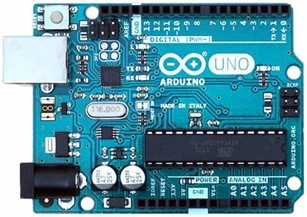
\includegraphics[width=5.5cm]{babII_ArduinoUno.jpg}
    \caption{Papan Mikrokontroler Arduino Uno R3 \cite{sunar2021}}
    \label{fig:arduino_uno}
\end{figure}

Arduino Uno merupakan papan mikrokontroler berbasis ATmega328P yang banyak digunakan dalam pengembangan proyek elektronika maupun instrumentasi. Tampilan fisik papan mikrokontroler Arduino Uno R3 ditunjukkan pada Gambar~\ref{fig:arduino_uno}. Papan ini memiliki 14 pin \textit{input/output} digital (6 di antaranya mendukung keluaran PWM) serta 6 pin masukan analog, dilengkapi osilator kristal 16 MHz, port USB, dan header ICSP \cite{sunar2021}. Bahasa pemrograman utamanya adalah C/C++ melalui Arduino IDE, dan papan ini dapat diintegrasikan dengan komputer host menggunakan Python melalui pustaka seperti \texttt{pySerial} \cite{sanjaya2025,dinata2016}. Pada penelitian ini, Arduino Uno berperan sebagai unit akuisisi yang membaca data digital dari ADC ADS1115 melalui antarmuka I2C dan meneruskannya melalui komunikasi serial ke Raspberry Pi.

\subsection{Raspberry Pi 5}
Raspberry Pi 5 adalah komputer papan tunggal generasi terbaru dari Raspberry Pi Ltd., menggunakan prosesor Broadcom BCM2712 \textit{quad-core} Arm Cortex-A76 64-bit berkecepatan 2,4 GHz, dengan peningkatan kinerja CPU 2--3 kali dibandingkan Raspberry Pi 4 \cite{raspberrypi2025}. Perangkat ini mendukung antarmuka USB, GPIO 40-pin, konektivitas Gigabit Ethernet dan Wi-Fi, serta mampu menjalankan sistem operasi berbasis Linux penuh, sehingga sesuai digunakan sebagai unit pengolah data tingkat tinggi (\textit{host}) yang menerima data mentah dari mikrokontroler dan menjalankan skrip Python untuk analisis serta penyimpanan data \cite{raspberrypi2025}.

\subsection{Sensor TMR ALT023-10E}
\begin{figure}[H]
    \centering
    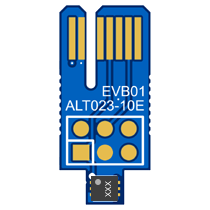
\includegraphics[width=4cm]{babII_ALT023.png}
    \caption{Modul Evaluasi Sensor TMR ALT023-10E (EVB01) \cite{nve_alt023_evb}}
    \label{fig:alt023}
\end{figure}

Sensor ALT023-10E adalah sensor magnetometer analog berbasis \textit{Tunneling Magnetoresistance} produksi NVE Corporation, dikemas dalam paket DFN6 berukuran 2,5$\times$2,5$\times$0,8 mm dengan resistansi divais 20 k$\Omega$ \cite{nve_alt023_evb}. Bentuk fisik modul evaluasi sensor TMR ALT023-10E (EVB01) ditunjukkan pada Gambar~\ref{fig:alt023}. Sensor ini memiliki keluaran jembatan diferensial bersifat \textit{bipolar} (positif untuk medan magnet satu arah, negatif untuk arah sebaliknya), dengan rentang medan linear $\pm$1 mT, medan saturasi sekitar 1,5 mT, sensitivitas tipikal 200 mV/V/mT (rentang 150--250 mV/V/mT), linearitas tipikal 0,1--0,2\% dari skala penuh, serta bandwidth hingga 300 kHz \cite{nve_alt023}. Sensor ini dapat dicatu pada rentang tegangan fleksibel 0--5,5 V tanpa batas minimum, menjadikannya kompatibel dengan catu daya tunggal 5 V yang digunakan pada instrumentasi penelitian ini \cite{magneticsmag_alt023}. Dibandingkan sensor GMR yang digunakan pada penelitian sebelumnya, ALT023-10E menawarkan sensitivitas per-volt-suplai yang jauh lebih tinggi, sebagaimana telah dibahas pada Subbab 2.1.2, sehingga berpotensi meningkatkan kemampuan sistem dalam mendeteksi perubahan medan magnet berskala kecil akibat interaksi formalin dengan nanofiber Fe$_3$O$_4$/PVA-ADH.

\subsection{IC AD623}
\begin{figure}[H]
    \centering
    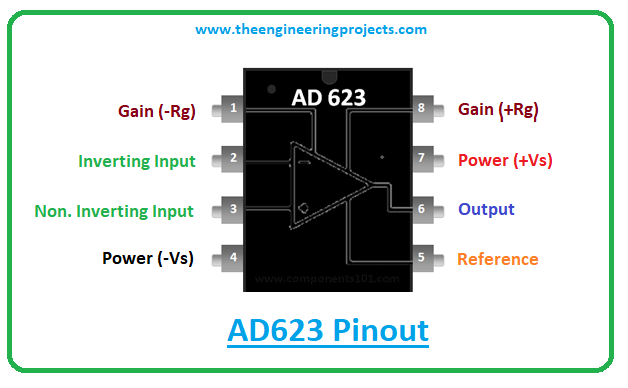
\includegraphics[width=6.5cm]{babII_AD623_Pinout.png}
    \caption{Konfigurasi Pin (\textit{Pinout}) IC \textit{Instrumentation Amplifier} AD623}
    \label{fig:ad623_pinout}
\end{figure}

AD623 adalah IC \textit{instrumentation amplifier} produksi Analog Devices yang dirancang untuk operasi catu daya tunggal maupun ganda, dengan rentang tegangan suplai 2,7--12 V dan keluaran \textit{rail-to-rail} \cite{adi_ad623}. Konfigurasi pin (\textit{pinout}) dari IC AD623 ditunjukkan pada Gambar~\ref{fig:ad623_pinout}. Penguatan (\textit{gain}) diatur melalui satu resistor eksternal $R_G$ yang dipasang antar-pin $-R_G$ dan $+R_G$, mengikuti persamaan
\begin{equation}
G = 1 + \frac{100\,\mathrm{k}\Omega}{R_G},
\label{eq:ad623_gain}
\end{equation}
dengan rentang gain dapat diatur dari 1 (tanpa resistor eksternal) hingga 1000 \cite{adi_ad623}. IC ini dilengkapi pin \texttt{REF} yang memungkinkan tegangan keluaran digeser ke titik referensi tertentu, sehingga sinyal bipolar kecil dari sensor TMR dapat diangkat ke rentang tegangan positif yang sesuai dengan input ADC catu daya tunggal. AD623 dipilih pada penelitian ini menggantikan IC LM358 yang digunakan pada instrumentasi GMR sebelumnya, karena AD623 secara khusus dirancang sebagai \textit{instrumentation amplifier} tiga op-amp dengan CMRR tinggi dan pengaturan gain satu-resistor, yang lebih sesuai untuk menguatkan sinyal diferensial kecil dari jembatan sensor magnetoresistif dibandingkan konfigurasi op-amp subtraktor diskret \cite{adi_ad623}.

\subsection{Resistor}
\begin{figure}[H]
    \centering
    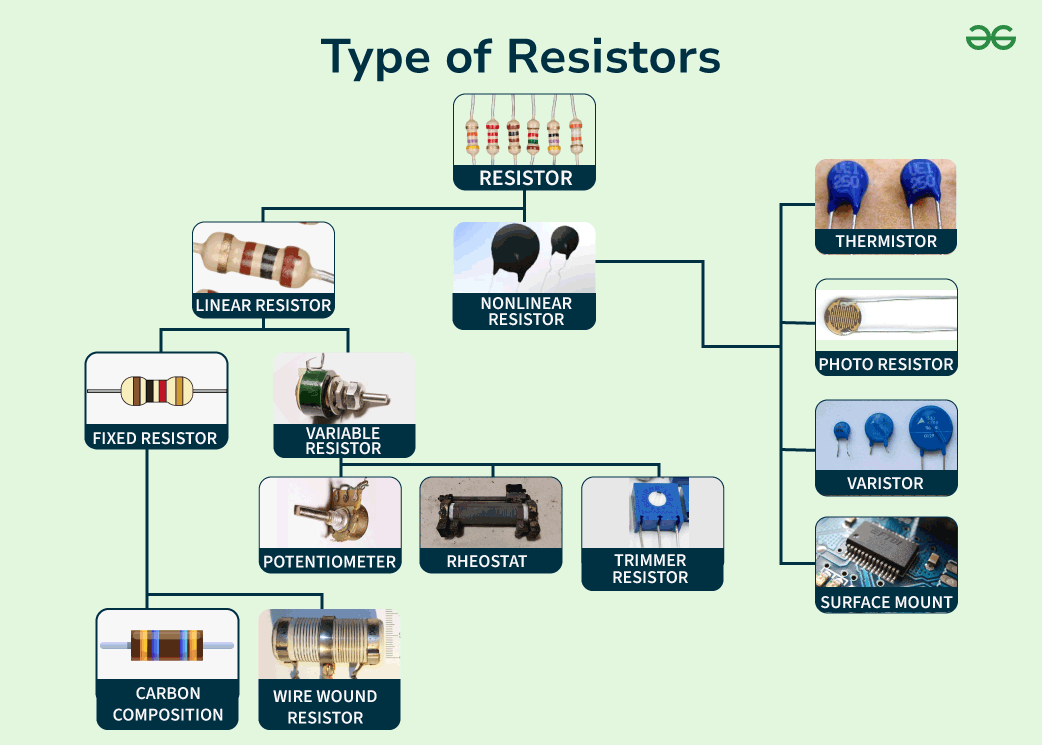
\includegraphics[width=7.5cm]{babII_Types-of-resistors.png}
    \caption{Klasifikasi dan Ragam Jenis Resistor \cite{electrical4u_resistor}}
    \label{fig:types_of_resistors}
\end{figure}

Resistor adalah komponen pasif dua terminal yang memberikan hambatan terhadap aliran arus listrik, berfungsi membatasi, mengatur, dan membagi arus dalam suatu rangkaian \cite{geeksforgeeks_resistor,electrical4u_resistor}. Klasifikasi dan jenis-jenis resistor ditampilkan pada Gambar~\ref{fig:types_of_resistors}. Resistor dikategorikan menjadi resistor tetap, dengan nilai resistansi tidak berubah (komposisi karbon, film, atau \textit{wire-wound}), dan resistor variabel yang nilainya dapat diubah, misalnya potensiometer \cite{circuitbasics_resistor}. Pada penelitian ini, resistor digunakan pada rangkaian filter RFI dan \textit{anti-aliasing}, pembagi tegangan referensi (\texttt{REF}) AD623, serta penentu gain ($R_G$).

\subsection{Kapasitor}
Kapasitor adalah komponen pasif yang menyimpan dan melepaskan energi listrik, tersusun dari dua elektroda konduktif yang dipisahkan medium isolator atau elektrolit \cite{liu2024review,sun2022review}. Kapasitor dielektrik (film, keramik, elektrolit) merupakan jenis yang umum digunakan pada rangkaian penyaringan sinyal dan stabilisasi daya \cite{liu2024review}. Pada penelitian ini, kapasitor digunakan pada rangkaian filter RFI di masukan AD623, filter \textit{anti-aliasing} sebelum ADC, serta \textit{decoupling} pada setiap jalur catu daya IC.

\subsection{ADC 16-bit ADS1115}
\begin{figure}[H]
    \centering
    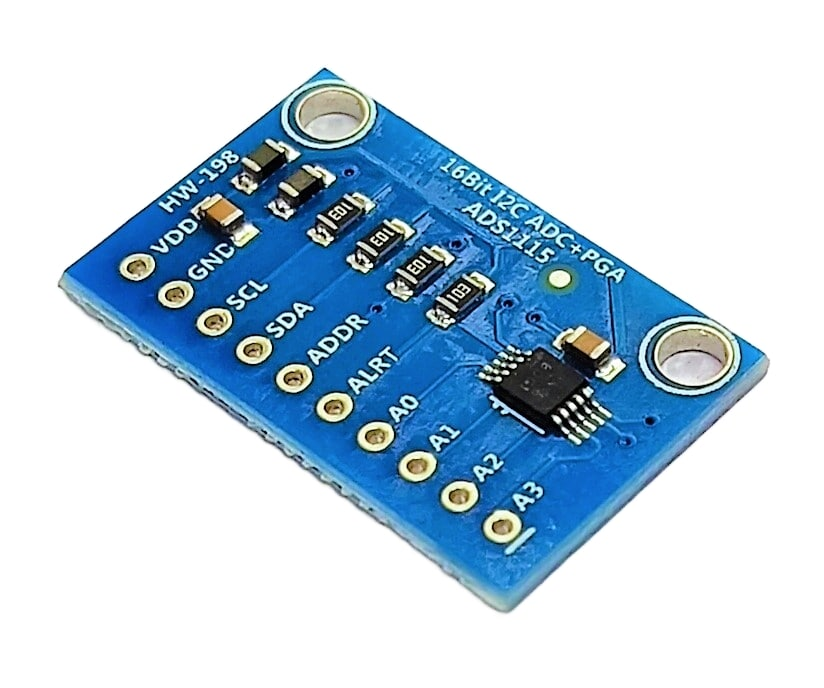
\includegraphics[width=5cm]{babII_ADS-1115-c.jpg}
    \caption{Modul ADC 16-bit ADS1115 \cite{adafruit_ads1115}}
    \label{fig:ads1115_modul}
\end{figure}

ADS1115 adalah ADC 16-bit berbasis arsitektur \textit{delta-sigma} produksi Texas Instruments, dengan konsumsi daya rendah dan referensi tegangan internal, sehingga sesuai untuk sistem instrumentasi presisi \cite{ti_ads1115}. Modul ADS1115 yang digunakan ditunjukkan pada Gambar~\ref{fig:ads1115_modul}. Perangkat ini mendukung empat kanal masukan \textit{single-ended} atau dua kanal diferensial, dilengkapi \textit{programmable gain amplifier} (PGA) dengan pilihan penguatan $\times$2/3, 1, 2, 4, 8, hingga 16, serta laju konversi yang dapat diprogram dari 8 hingga 860 sampel per detik (SPS) \cite{adafruit_ads1115}. Komunikasi dilakukan melalui antarmuka I2C dengan hingga empat alamat berbeda (0x48--0x4B) yang dipilih melalui pin \texttt{ADDR}, serta pin \texttt{ALERT/RDY} yang dapat difungsikan sebagai indikator kesiapan data \cite{ti_ads1115}. Pada penelitian ini, ADS1115 membaca keluaran AD623 pada kanal AIN0 secara \textit{single-ended}, dengan PGA diatur pada rentang skala penuh $\pm$6,144 V agar seluruh rentang keluaran AD623 (0--5 V) dapat terbaca tanpa \textit{clipping}.
%\chapter{PROFIL INDUSTRI}

\section{Profil Bolabot \textit{Techno Robotics Institute}}
Bolabot \textit{Techno Robotics Institute} merupakan institusi yang mengutamakan riset dan pendidikan di bidang teknologi robotika. Lembaga ini secara aktif melakukan penelitian yang mencakup otomasi perangkat, pengendalian alat, pemrosesan sinyal, penerapan kecerdasan buatan, sistem penglihatan untuk robot, serta instrumentasi dalam pengukuran alat-alat fisika \cite{15}.

Tidak hanya terbatas pada riset, institusi ini juga menyelenggarakan program pendidikan robotika bagi berbagai jenjang, mulai dari tingkat sekolah dasar hingga perguruan tinggi, serta menyediakan pelatihan khusus bagi para guru. Selain itu, Bolabot \textit{Techno Robotics Institute} mengembangkan beragam perangkat yang mendukung kegiatan praktikum pada mata pelajaran Elektronika Dasar, Fisika Dasar, dan Fisika Komputasi \cite{15}.

Di samping fungsinya sebagai perusahaan yang berfokus pada riset dan pendidikan, lembaga ini juga berhasil membentuk komunitas yang mengakomodasi antusiasme masyarakat terhadap robotika. Komunitas tersebut pertama kali didirikan pada tahun 2014 dengan nama \textit{“Physics of Instrumentation and Computation Organization”} (PICO), dan kemudian mengalami perubahan nama pada pertengahan tahun 2015 menjadi “Komunitas Pecinta Robot” (KOTARO) \cite{15}.

\section{Sejarah Bolabot \textit{Techno Robotic Institute}}
BOLABOT bermula dari komunitas riset di bidang komputasi dan instrumentasi yang dibentuk di lingkungan Fisika UIN Sunan Gunung Djati Bandung sejak tahun 2010. Inisiatif awal ini diprakarsai oleh beberapa tokoh kunci, yaitu Mada Sanjaya W.S., Dian Syah Maulana, Halimatussadiyah, Okyza Maherdi P, Irfan Syafar Farouk, Sandy Yusuf, Utin Sutinah, serta Aah Kholifah. Seiring berjalannya waktu, Irawan Febrianto sebagai alumni Instrumentasi UIN SGD angkatan 2008 dan 2009—bergabung untuk semakin memperkuat fondasi komunitas ini \cite{15}.

BOLABOT secara resmi mulai beroperasi pada tanggal 11 Maret 2012 di bawah payung hukum CV. Sanjaya Star Group, yang menandai dimulainya perjalanan strategis dalam bidang riset dan inovasi robotika. Kegiatan awal yang dilaksanakan meliputi penyelenggaraan program pembelajaran robotika secara reguler dan privat, pengembangan projek alat praktikum dalam mata pelajaran elektronika dasar, serta penyelenggaraan seminar dan workshop yang mendalami aspek teknologi robotika. Selanjutnya, upaya perluasan dampak pendidikan diwujudkan melalui pengenalan ekstrakurikuler robotika di berbagai sekolah. Pada bulan Desember 2012, BOLABOT bersama dengan Robotika UIN meluncurkan event Robocom Pertama, yang mencakup kompetisi robotik. Acara tersebut terbagi dalam dua segmen, yakni lomba robot \textit{line follower} analog bagi siswa binaan BOLABOT dan kompetisi \textit{robot soccer} digital yang melibatkan mahasiswa pada mata kuliah elektronika dasar Fisika Sains UIN Sunan Gunung Djati Bandung \cite{15}.

Lebih lanjut, pada tanggal 10 November 2014, terbentuklah komunitas khusus mahasiswa Instrumentasi Fisika UIN SGD dengan nama PICO \textit{(Physics Instrumentation and Computation Organization)}. Komunitas ini kemudian mengalami transformasi pada bulan Juli 2015 dan berganti nama menjadi KoTaRo (Komunitas Pecinta Robot), sebagai salah satu divisi sosial BOLABOT yang bertujuan untuk menyebarluaskan pengetahuan robotika secara lebih luas di Indonesia. Sejalan dengan dinamika strategis organisasi, pada tahun 2018 terjadi perubahan struktural di mana CV. Sanjaya Star Group secara resmi diubah menjadi CV. BOLABOT. Pada tahun yang sama, Divisi Publikasi Riset mendirikan penerbitan buku ilmiah yang dinamakan Penerbit BOLABOT. Inisiatif ini memungkinkan lembaga untuk menerbitkan karya ilmiah hasil riset internal maupun karya dari penulis lain, yang kemudian dapat dipasarkan secara komersial, memperkuat posisi BOLABOT sebagai pionir dalam riset dan inovasi di bidang robotika \cite{15}.

\section{Visi dan Misi Bolabot \textit{Techno Robotics Institute}}

\subsection{Visi Bolabot \textit{Techno Robotics Institute}}
Visi dari Bolabot \textit{Techno Robotics Institute} adalah menjadi ikon perusahaan berbasis edukasi, riset, dan teknologi robotika di Indonesia \cite{15}.

\subsection{Misi Bolabot \textit{Techno Robotics Institute}}
Misi dari Bolabot \textit{Techno Robotics Institute} adalah sebagai berikut \cite{6}:
\begin{enumerate}
    \item Mengembangkan pendidikan robotik yang menarik, kreatif, dan menyenangkan.
    \item Menyelenggarakan pendidikan nonformal sebagai penunjang kecakapan dan pembelajaran.
    \item Melakukan berbagai penelitian untuk menciptakan inovasi teknologi.
    \item Menciptakan berbagai produk untuk memenuhi kebutuhan pendidikan dan industri.
    \item Menciptakan usaha-usaha baru di bidang teknologi.
\end{enumerate}


\section{Roadmap Bolabot \textit{Techno Robotics Institute}}

Terdapat tiga bidang utama dan satu bidang sosial yang menjadi target kerja Bolabot, yaitu sebagai berikut \cite{15}:

\begin{enumerate}
    \item \textbf{Bidang Edukasi Robotika}: Menyelenggarakan pendidikan dan pelatihan pembuatan robot secara reguler, membina ekstrakurikuler robotika, serta mengadakan workshop dan seminar robotika.
    \item \textbf{Bidang Produksi Robotika}: Memproduksi kit edukasi robotika, kit praktikum berbasis komputer, serta kit otomatisasi untuk pesanan umum.
    \item \textbf{Bidang Media dan Publikasi Robotika}: Menulis buku-buku robotika, mempublikasikan hasil riset, membuat modul belajar robotika, dan memberikan edukasi robotika kepada masyarakat melalui platform digital.
    \item \textbf{Bidang Sosial dan Edukasi Masyarakat}: Membangun komunitas-komunitas robotika di kampus dan sekolah melalui program KoTaRo.
\end{enumerate}


\chapter{METODE PENELITIAN}

\section{Waktu dan Tempat Penelitian}
Penelitian \textquotedblleft Rancang Bangun Instrumentasi Sensor \textit{Tunneling Magnetoresistance} Berbasis Nanofiber \ch{Fe3O4}/PVA-Sitrat-ADH untuk Deteksi Formalin pada Bakso Menggunakan Komparasi Model Klasik (SVM, Random Forest) dan Kuantum (QSVC, VQC)\textquotedblright\ akan dilaksanakan pada bulan September--Desember 2026, bertempat di Kantor Bolabot \textit{Techno Robotic Institute,} Jl. Sauyunan VI No. 10 Blok F6, Kelurahan Cipadung, Kecamatan Panyileukan, Kota Bandung, Jawa Barat 40614.

\section{Alat dan Bahan}
\subsection{Alat Penelitian}
Adapun alat yang digunakan pada proses penelitian adalah sebagai berikut.

\begin{singlespace}
\small
\begin{longtable}{|c|p{9.0cm}|c|}
    \caption{Alat yang Digunakan dalam Penelitian} \label{tab:alatbahan} \\
    \hline
    No. & Alat & Jumlah \\ \hline
    \endfirsthead
    
    \multicolumn{3}{c}{\small\textit{Lanjutan Tabel \ref{tab:alatbahan} Alat yang Digunakan dalam Penelitian}} \\[0.15cm]
    \hline
    No. & Alat & Jumlah \\ \hline
    \endhead
    
    \hline
    \endfoot
    
    \hline
    \endlastfoot
    
    1.  & Mesin \textit{Laser Cutting}           & 1 set \\ \hline
    2.  & Raspberry Pi 5 dan Monitor             & 1 kit \\ \hline
    3.  & Solder                                 & 1 buah \\ \hline
    4.  & Tang Pemotong                          & 1 buah \\ \hline
    5.  & Gunting                                & 1 buah \\ \hline
    6.  & Obeng                                  & 1 buah \\ \hline
    7.  & Mikropipet                             & 1 buah \\ \hline
    8.  & \textit{Tweezer} Pencapit              & 1 buah \\ \hline
    9.  & Timbangan Digital                      & 1 buah \\ \hline
    10. & Sonikator                              & 1 buah \\ \hline
    11. & \textit{Electrospinning}               & 1 kit \\ \hline
    12. & \textit{Magnetic Stirrer}              & 1 kit \\ \hline
    13. & Spatula                                & 1 buah \\ \hline
    14. & \textit{Magnetic Bar}                  & 1 buah \\ \hline
    15. & Vial                                   & Secukupnya \\ \hline
    16. & Gelas Ukur                             & 1 buah \\ \hline
    17. & \textit{Fume Hood}                     & 1 buah \\ \hline
    18. & Gaussmeter / Teslameter                & 1 buah \\ \hline
    19. & Catu Daya                              & 1 buah \\ \hline
    20. & Oven Pengering / \textit{Vacuum Oven}  & 1 buah \\ \hline
\end{longtable}
\end{singlespace}

Tabel~\ref{tab:alatbahan} merinci peralatan yang digunakan dalam penelitian ini. Perangkat fabrikasi dan karakterisasi utama mencakup unit \textit{electrospinning} untuk penarikan serat nano komposit, sonikator dan \textit{magnetic stirrer} untuk homogenisasi larutan prekursor, \textit{fume hood} untuk menjamin keselamatan reaksi kimia sintesis, serta oven pengering untuk aktivasi \textit{thermal curing} asam sitrat pada suhu $130\,^{\circ}\text{C}$. Pada sistem instrumentasi, kumparan Helmholtz dan teslameter digunakan sebagai sumber serta acuan medan magnet kalibrasi, sedangkan Raspberry Pi 5 terintegrasi monitor berfungsi sebagai unit pemroses utama data akuisisi secara \textit{realtime}.

\begin{singlespace}
\small
\begin{longtable}{|c|p{3.2cm}|c|c|p{5.5cm}|}
    \caption{Perangkat Lunak (\textit{Software}) yang Digunakan} \label{tab:software} \\
    \hline
    No. & Nama Perangkat & Tipe & Lisensi & Kegunaan \\ \hline
    \endfirsthead
    
    \multicolumn{5}{c}{\small\textit{Lanjutan Tabel \ref{tab:software} Perangkat Lunak (\textit{Software}) yang Digunakan}} \\[0.15cm]
    \hline
    No. & Nama Perangkat & Tipe & Lisensi & Kegunaan \\ \hline
    \endhead
    
    \hline
    \endfoot
    
    \hline
    \endlastfoot
    
    1.  & Arduino IDE 2.3.4       & EXE     & Freeware & Pemrograman mikrokontroler Arduino \\ \hline
    2.  & Python 3.12.10          & EXE     & Freeware & Bahasa pemrograman analisis data \& integrasi \\ \hline
    3.  & matplotlib 3.7.1        & Package & Freeware & Visualisasi grafik dan kurva kalibrasi \\ \hline
    4.  & tk 0.1.0                & Package & Freeware & Antarmuka GUI (\textit{Graphical User Interface}) \\ \hline
    5.  & pyserial 3.5            & Package & Freeware & Komunikasi serial Arduino dan Python \\ \hline
    6.  & pandas 2.2.3            & Package & Freeware & Pengelolaan dan manipulasi data tabular \\ \hline
    7.  & scikit-learn 1.6.1      & Package & Freeware & Analisis data dan pemodelan klasik (SVM, RF) \\ \hline
    8.  & numpy 1.26.4            & Package & Freeware & Perhitungan numerik larik multidimensi \\ \hline
    9.  & scipy 1.15.3            & Package & Freeware & Komputasi ilmiah dan analisis statistik \\ \hline
    10. & Qiskit 1.0.2            & Package & Freeware & Perancangan sirkuit dan simulasi kuantum \\ \hline
    11. & Qiskit ML 0.7.2         & Package & Freeware & Implementasi model kuantum (QSVC, VQC) \\ \hline
    12. & CorelDraw 2019          & ZIP     & Freeware & Desain mekatronika 2D casing instrumen \\ \hline
    13. & LaserDRW 2013.02        & EXE     & Freeware & Eksekusi pemotongan casing pada mesin laser \\ \hline
\end{longtable}
\end{singlespace}

Tabel~\ref{tab:software} merangkum perangkat lunak dan pustaka komputasi yang digunakan. Arduino IDE berperan dalam pemrograman mikrokontroler untuk akuisisi data mentah, sedangkan lingkungan Python yang didukung pustaka \textit{pyserial}, \textit{pandas}, \textit{numpy}, dan \textit{scipy} digunakan untuk komunikasi serial, pengolahan statistik, dan analisis regresi kalibrasi. Penerapan model pembelajaran mesin klasik (SVM dan RF) didukung oleh pustaka \textit{scikit-learn}, sedangkan implementasi model kuantum (QSVC dan VQC) dibangun menggunakan pustaka \textit{Qiskit} dan \textit{Qiskit Machine Learning}. Perancangan fisik casing instrumen dirancang menggunakan CorelDraw dan diproduksi melalui LaserDRW. Seluruh perangkat lunak ini terintegrasi dalam alur rancang bangun dan pengujian performa sistem instrumentasi sensor TMR.

\subsection{Bahan Penelitian}
Adapun bahan yang digunakan dalam penelitian adalah sebagai berikut.

\begin{singlespace}
\small
\begin{longtable}{|c|p{9.0cm}|c|}
    \caption{Bahan yang Digunakan dalam Penelitian} \label{tab:bahan} \\
    \hline
    No. & Bahan & Jumlah \\ \hline
    \endfirsthead
    
    \multicolumn{3}{c}{\small\textit{Lanjutan Tabel \ref{tab:bahan} Bahan yang Digunakan dalam Penelitian}} \\[0.15cm]
    \hline
    No. & Bahan & Jumlah \\ \hline
    \endhead
    
    \hline
    \endfoot
    
    \hline
    \endlastfoot
    
    1.  & Sensor TMR ALT023-10E (EVB01)                  & 1 buah \\ \hline
    2.  & IC \textit{Instrumentation Amplifier} AD623    & 1 buah \\ \hline
    3.  & Resistor 1 k$\Omega$ (filter RFI \& pembagi bias \texttt{REF}) & 4 buah \\ \hline
    4.  & Resistor 10 k$\Omega$ ($R_G$ gain AD623 \& filter pasif LPF)  & 2 buah \\ \hline
    5.  & Resistor 4,7 k$\Omega$ (\textit{pull-up} I2C)  & 2 buah \\ \hline
    6.  & Kapasitor 100 nF (C0G/NP0)                     & Secukupnya \\ \hline
    7.  & Kapasitor 10 nF                                & 2 buah \\ \hline
    8.  & Kapasitor elektrolitik 10 $\mu$F               & 1 buah \\ \hline
    9.  & ADC ADS1115 16-bit                             & 1 buah \\ \hline
    10. & Arduino Uno R3                                 & 1 buah \\ \hline
    11. & PCB Kit Instrumentasi                          & 1 buah \\ \hline
    12. & Timah solder                                   & Secukupnya \\ \hline
    13. & \ch{FeSO4} (prekursor sintesis \ch{Fe3O4})     & 7,5 mL \\ \hline
    14. & \ch{FeCl3} (prekursor sintesis \ch{Fe3O4})     & 7,5 mL \\ \hline
    15. & Ekstrak \textit{Moringa oleifera} (MO)         & 10 mL \\ \hline
    16. & \ch{NH4OH} (amonia)                            & 12 mL \\ \hline
    17. & Aquades                                        & Secukupnya \\ \hline
    18. & PVA (\textit{Polyvinyl Alcohol})               & 0,55 gram \\ \hline
    19. & Serbuk \ch{Fe3O4} hasil sintesis               & 0,2 gram \\ \hline
    20. & Asam Sitrat (\textit{Citric Acid}, pro-analisis)& Secukupnya \\ \hline
    21. & ADH (\textit{Adipic Acid Dihydrazide})         & Secukupnya \\ \hline
    22. & Etanol                                         & Secukupnya \\ \hline
    23. & Aluminium foil ($20 \times 10$ cm)             & Secukupnya \\ \hline
    24. & Tape perekat                                   & Secukupnya \\ \hline
    25. & Larutan formalin standar (37\%)                & Secukupnya \\ \hline
    26. & Sampel bakso (kontrol \& uji)                  & Secukupnya \\ \hline
\end{longtable}
\end{singlespace}

Tabel~\ref{tab:bahan} merinci bahan kimia dan komponen perangkat keras yang digunakan dalam penelitian ini. Pada bagian perangkat keras, sensor TMR ALT023-10E berperan sebagai transduser \textit{tunneling magnetoresistance} yang sensitif terhadap perubahan medan magnet. Rangkaian pengkondisi sinyal menggunakan IC AD623 sebagai \textit{instrumentation amplifier}, didukung oleh resistor 1~k$\Omega$ untuk filter RFI dan pembagi tegangan referensi, serta resistor $R_G = 10{,}0\,\text{k}\Omega$ penentu penguatan ($G = 11$). Kapasitor 100~nF dan 10~nF ditambahkan sebagai filter RFI dan \textit{anti-aliasing} untuk mereduksi derau. Konversi sinyal analog ke digital dilakukan oleh ADC ADS1115 dengan resolusi 16-bit, yang hasilnya kemudian diproses oleh mikrokontroler Arduino Uno R3 melalui antarmuka I2C. Kit instrumentasi terintegrasi pada satu PCB cetak dan direkatkan dengan timah. Pada aspek bahan kimia, PVA digunakan sebagai polimer dasar pembentuk serat, \ch{Fe3O4} berfungsi sebagai partikel magnetik superparamagnetik utama, asam sitrat berperan ganda sebagai agen penstabil dispersi (\textit{capping agent}) nanopartikel sekaligus agen penaut silang hijau tunggal (\textit{green crosslinker}) melalui esterifikasi termal, dan ADH berfungsi khusus sebagai molekul pengenal (\textit{chemo-receptor}) yang menyediakan gugus hidrazida terminal bebas untuk mengikat analit formaldehida secara kovalen. Aquades berperan sebagai pelarut, sedangkan aluminium foil dan perekat digunakan sebagai media kolektor \textit{electrospinning}. Kombinasi material ini menghasilkan nanofiber \ch{Fe3O4}/PVA-Sitrat-ADH yang menjadi elemen reseptor pada sensor TMR. Larutan formalin standar digunakan sebagai analit acuan untuk kalibrasi sistem, sedangkan sampel bakso (kontrol tanpa formalin dan uji mengandung formalin) digunakan sebagai sampel riil untuk validasi kemampuan deteksi sensor.

\section{Metode Penelitian}
Penelitian ini diawali dengan studi literatur dari berbagai sumber untuk memperoleh informasi dan referensi yang relevan dalam mendukung pengembangan kit instrumentasi sensor TMR. Tahap berikutnya adalah analisis permasalahan untuk mengidentifikasi kebutuhan, keterbatasan, serta solusi yang dapat ditawarkan melalui sistem yang dirancang. Selanjutnya, dilakukan perancangan perangkat keras yang mencakup desain mekatronika casing serta rangkaian pengkondisi sinyal sensor TMR ALT023-10E. Setelah itu, dilanjutkan dengan perancangan perangkat lunak yang terdiri atas firmware Arduino untuk akuisisi data mentah dan skrip Python pada Raspberry Pi untuk pengendalian kalibrasi, pengolahan statistik, serta pemodelan. Setelah perancangan sistem, penelitian memasuki tahapan sintesis material. Tahapan ini meliputi sintesis nanopartikel \ch{Fe3O4}, pembuatan nanofiber \ch{Fe3O4}/PVA menggunakan metode \textit{electrospinning}, penautan silang (\textit{crosslinking}) melalui \textit{thermal curing} asam sitrat pada suhu $130\,^{\circ}\text{C}$, serta fungsionalisasi permukaan dengan ADH sebagai situs pengenalan formaldehida. Pada tahap pengujian, sistem diuji secara komprehensif: (1) uji kalibrasi medan magnet kumparan Helmholtz, (2) uji respons dan sensitivitas sensor TMR terhadap medan magnet acuan, (3) uji respons sensor terhadap variasi konsentrasi larutan formalin standar, (4) uji pada sampel bakso riil (kontrol dan uji), serta (5) ekstraksi fitur sinyal dan komparasi pemodelan dua model klasik (SVM dan RF) versus dua model kuantum (QSVC dan VQC). Seluruh rangkaian tahapan penelitian ini dirangkum dalam bentuk diagram alir yang ditunjukkan pada Gambar~\ref{fig:diagram_alir_penelitian}.

\begin{figure}[H]
    \centering
    \begin{tikzpicture}[node distance=0.65cm,
        block/.style={rectangle, rounded corners=4pt, minimum width=10cm, minimum height=0.85cm, text centered, text width=9.5cm, draw=black!70, fill=blu!60, font=\small},
        arr/.style={thick,->,>=stealth}]
        \node[block] (s1) {1. Studi Literatur dan Perumusan Masalah};
        \node[block, below=of s1] (s2) {2. Perancangan Perangkat Keras dan Rantai Sinyal TMR\\(ALT023-10E $\rightarrow$ AD623 $\rightarrow$ LPF $\rightarrow$ ADS1115 $\rightarrow$ Arduino)};
        \node[block, below=of s2] (s3) {3. Perancangan Perangkat Lunak Akuisisi Data\\(Firmware Arduino dan GUI Python)};
        \node[block, below=of s3] (s4) {4. Sintesis Nanofiber \ch{Fe3O4}/PVA-Sitrat-ADH\\(\textit{Electrospinning} + \textit{Thermal Curing} $130\,^{\circ}\text{C}$)};
        \node[block, below=of s4] (s5) {5. Karakterisasi Fisik Sensor terhadap Medan Magnet\\Acuan Helmholtz ($V$-$B$ dan $dV/dB$)};
        \node[block, below=of s5] (s6) {6. Pengujian Respons Sensor terhadap Larutan Formalin\\Standar dan Ekstrak Sampel Bakso};
        \node[block, below=of s6] (s7) {7. Ekstraksi Fitur Sinyal dan Komparasi Model\\Klasik (SVM, RF) vs Kuantum (QSVC, VQC)};
        \node[block, below=of s7] (s8) {8. Evaluasi Performa Sistem, Analisis Data, dan Kesimpulan};
        \foreach \i/\j in {s1/s2, s2/s3, s3/s4, s4/s5, s5/s6, s6/s7, s7/s8}
            \draw[arr] (\i) -- (\j);
    \end{tikzpicture}
    \caption{Diagram Alir Penelitian \textquotedblleft Rancang Bangun Instrumentasi Sensor \textit{Tunneling Magnetoresistance} Berbasis Nanofiber \ch{Fe3O4}/PVA-Sitrat-ADH untuk Deteksi Formalin pada Bakso Menggunakan Komparasi Model Klasik (SVM, Random Forest) dan Kuantum (QSVC, VQC)\textquotedblright}
    \label{fig:diagram_alir_penelitian}
\end{figure}

\subsection{Studi Literatur}
Studi literatur dilakukan secara komprehensif melalui penelaahan jurnal ilmiah terindeks, prosiding internasional, dan pustaka akademik terkait. Informasi yang dihimpun mencakup prinsip kerja sensor \textit{Tunneling Magnetoresistance} (TMR) dalam mendeteksi perubahan medan magnet, sintesis nanomaterial \ch{Fe3O4}/PVA-Sitrat-ADH sebagai reseptor selektif formaldehida, metode preparasi sampel bakso, serta landasan matematis pemodelan komparatif model klasik (SVM dan RF) dan model kuantum (QSVC dan VQC). Selain itu, dikaji pula metode kalibrasi medan magnet berbasis kumparan Helmholtz serta teknik evaluasi sensitivitas sensor guna menetapkan batas deteksi (LOD) yang akurat. Studi literatur ini menjadi landasan teoretis dan metodologis dalam perancangan keseluruhan sistem.

\subsection{Analisis Permasalahan}
Sistem instrumentasi sensor TMR untuk deteksi formalin pada bakso ini dirancang dengan dua program utama yang saling terintegrasi. Program pertama dikembangkan menggunakan Arduino IDE untuk mengendalikan mikrokontroler yang berfungsi sebagai pusat akuisisi data. Mikrokontroler bertugas membaca sinyal keluaran dari sensor \textit{Tunneling Magnetoresistance} (TMR) ALT023-10E melalui ADC ADS1115, mengatur kondisi pengukuran, serta mengalirkan data mentah secara kontinu melalui komunikasi serial. Program kedua dibangun menggunakan bahasa pemrograman Python, yang digunakan untuk menjalankan proses pengujian, akuisisi, dan analisis data secara otomatis. Melalui komunikasi serial, Python menerima data hasil pembacaan sensor dari mikrokontroler, kemudian menyimpan data tersebut ke dalam format terstruktur (CSV) dan menampilkan visualisasi hasil pengukuran secara \textit{realtime} pada antarmuka grafis (\textit{GUI}). Data yang direkam meliputi respons sensor terhadap variasi konsentrasi formalin, baik dalam bentuk larutan standar maupun dalam ekstrak sampel bakso. Selanjutnya, data hasil pengukuran diproses dengan model klasik (\textit{Support Vector Machine} dan \textit{Random Forest}) serta model kuantum (\textit{Quantum Support Vector Classifier} dan \textit{Variational Quantum Classifier}) untuk menganalisis sensitivitas, linearitas, serta akurasi deteksi formalin. Perbandingan kinerja antara kedua paradigma pemodelan menjadi kebaruan analitis utama dari penelitian ini.

\subsection{Perancangan Mekatronika Perangkat Keras}
\begin{figure}[H]
    \centering
    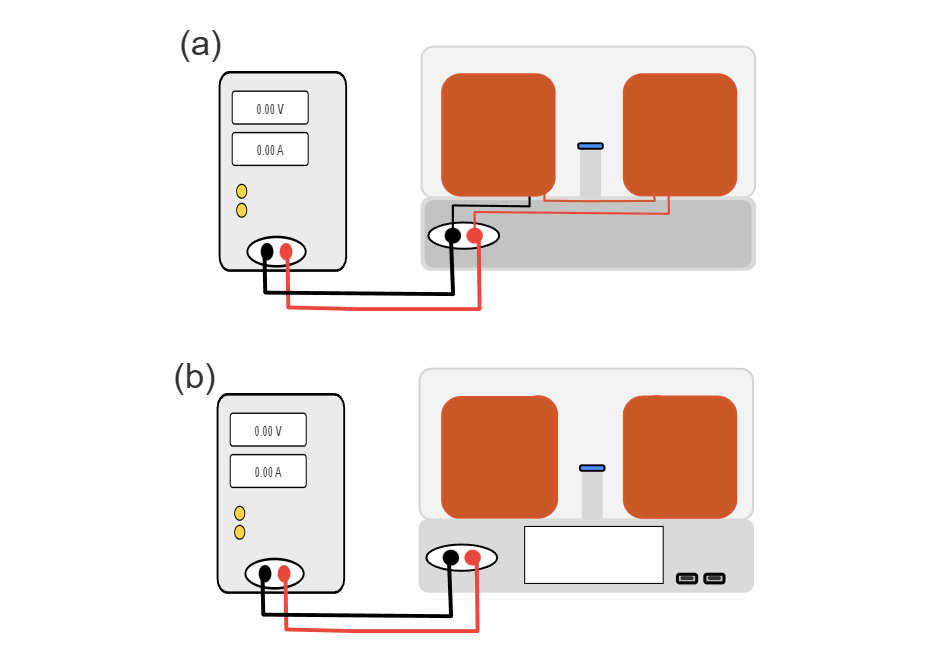
\includegraphics[width=0.75\linewidth]{babIII-desainTMR.png}
    \caption{Desain Prototipe Mekatronika Kit Instrumentasi Sensor TMR: (a) Tampak Dalam dengan Kumparan Helmholtz dan Sensor TMR, (b) Tampak Luar Terintegrasi dengan Catu Daya}
    \label{fig:desain_mekatronika}
\end{figure}

Gambar~\ref{fig:desain_mekatronika} merepresentasikan prototipe desain mekatronika perangkat keras kit instrumentasi sensor TMR. Tampilan (a) memperlihatkan struktur dalam dengan kumparan Helmholtz yang mengapit sensor TMR di area medan seragam, terhubung ke terminal daya eksternal. Tampilan (b) memperlihatkan tampilan muka instrumen dengan integrasi layar interaktif untuk kontrol sistem dan penampil hasil uji, soket catu daya kumparan Helmholtz, serta porta komunikasi periferal. Adapun realisasi fisik desain prototipe tersebut ditampilkan dalam Gambar~\ref{fig:realisasi_casing}, yang merinci Gambar~\ref{fig:realisasi_luar} (tampak luar) dan Gambar~\ref{fig:realisasi_dalam} (tampak dalam).

\begin{figure}[H]
    \centering
    \begin{subfigure}[b]{0.48\textwidth}
        \centering
        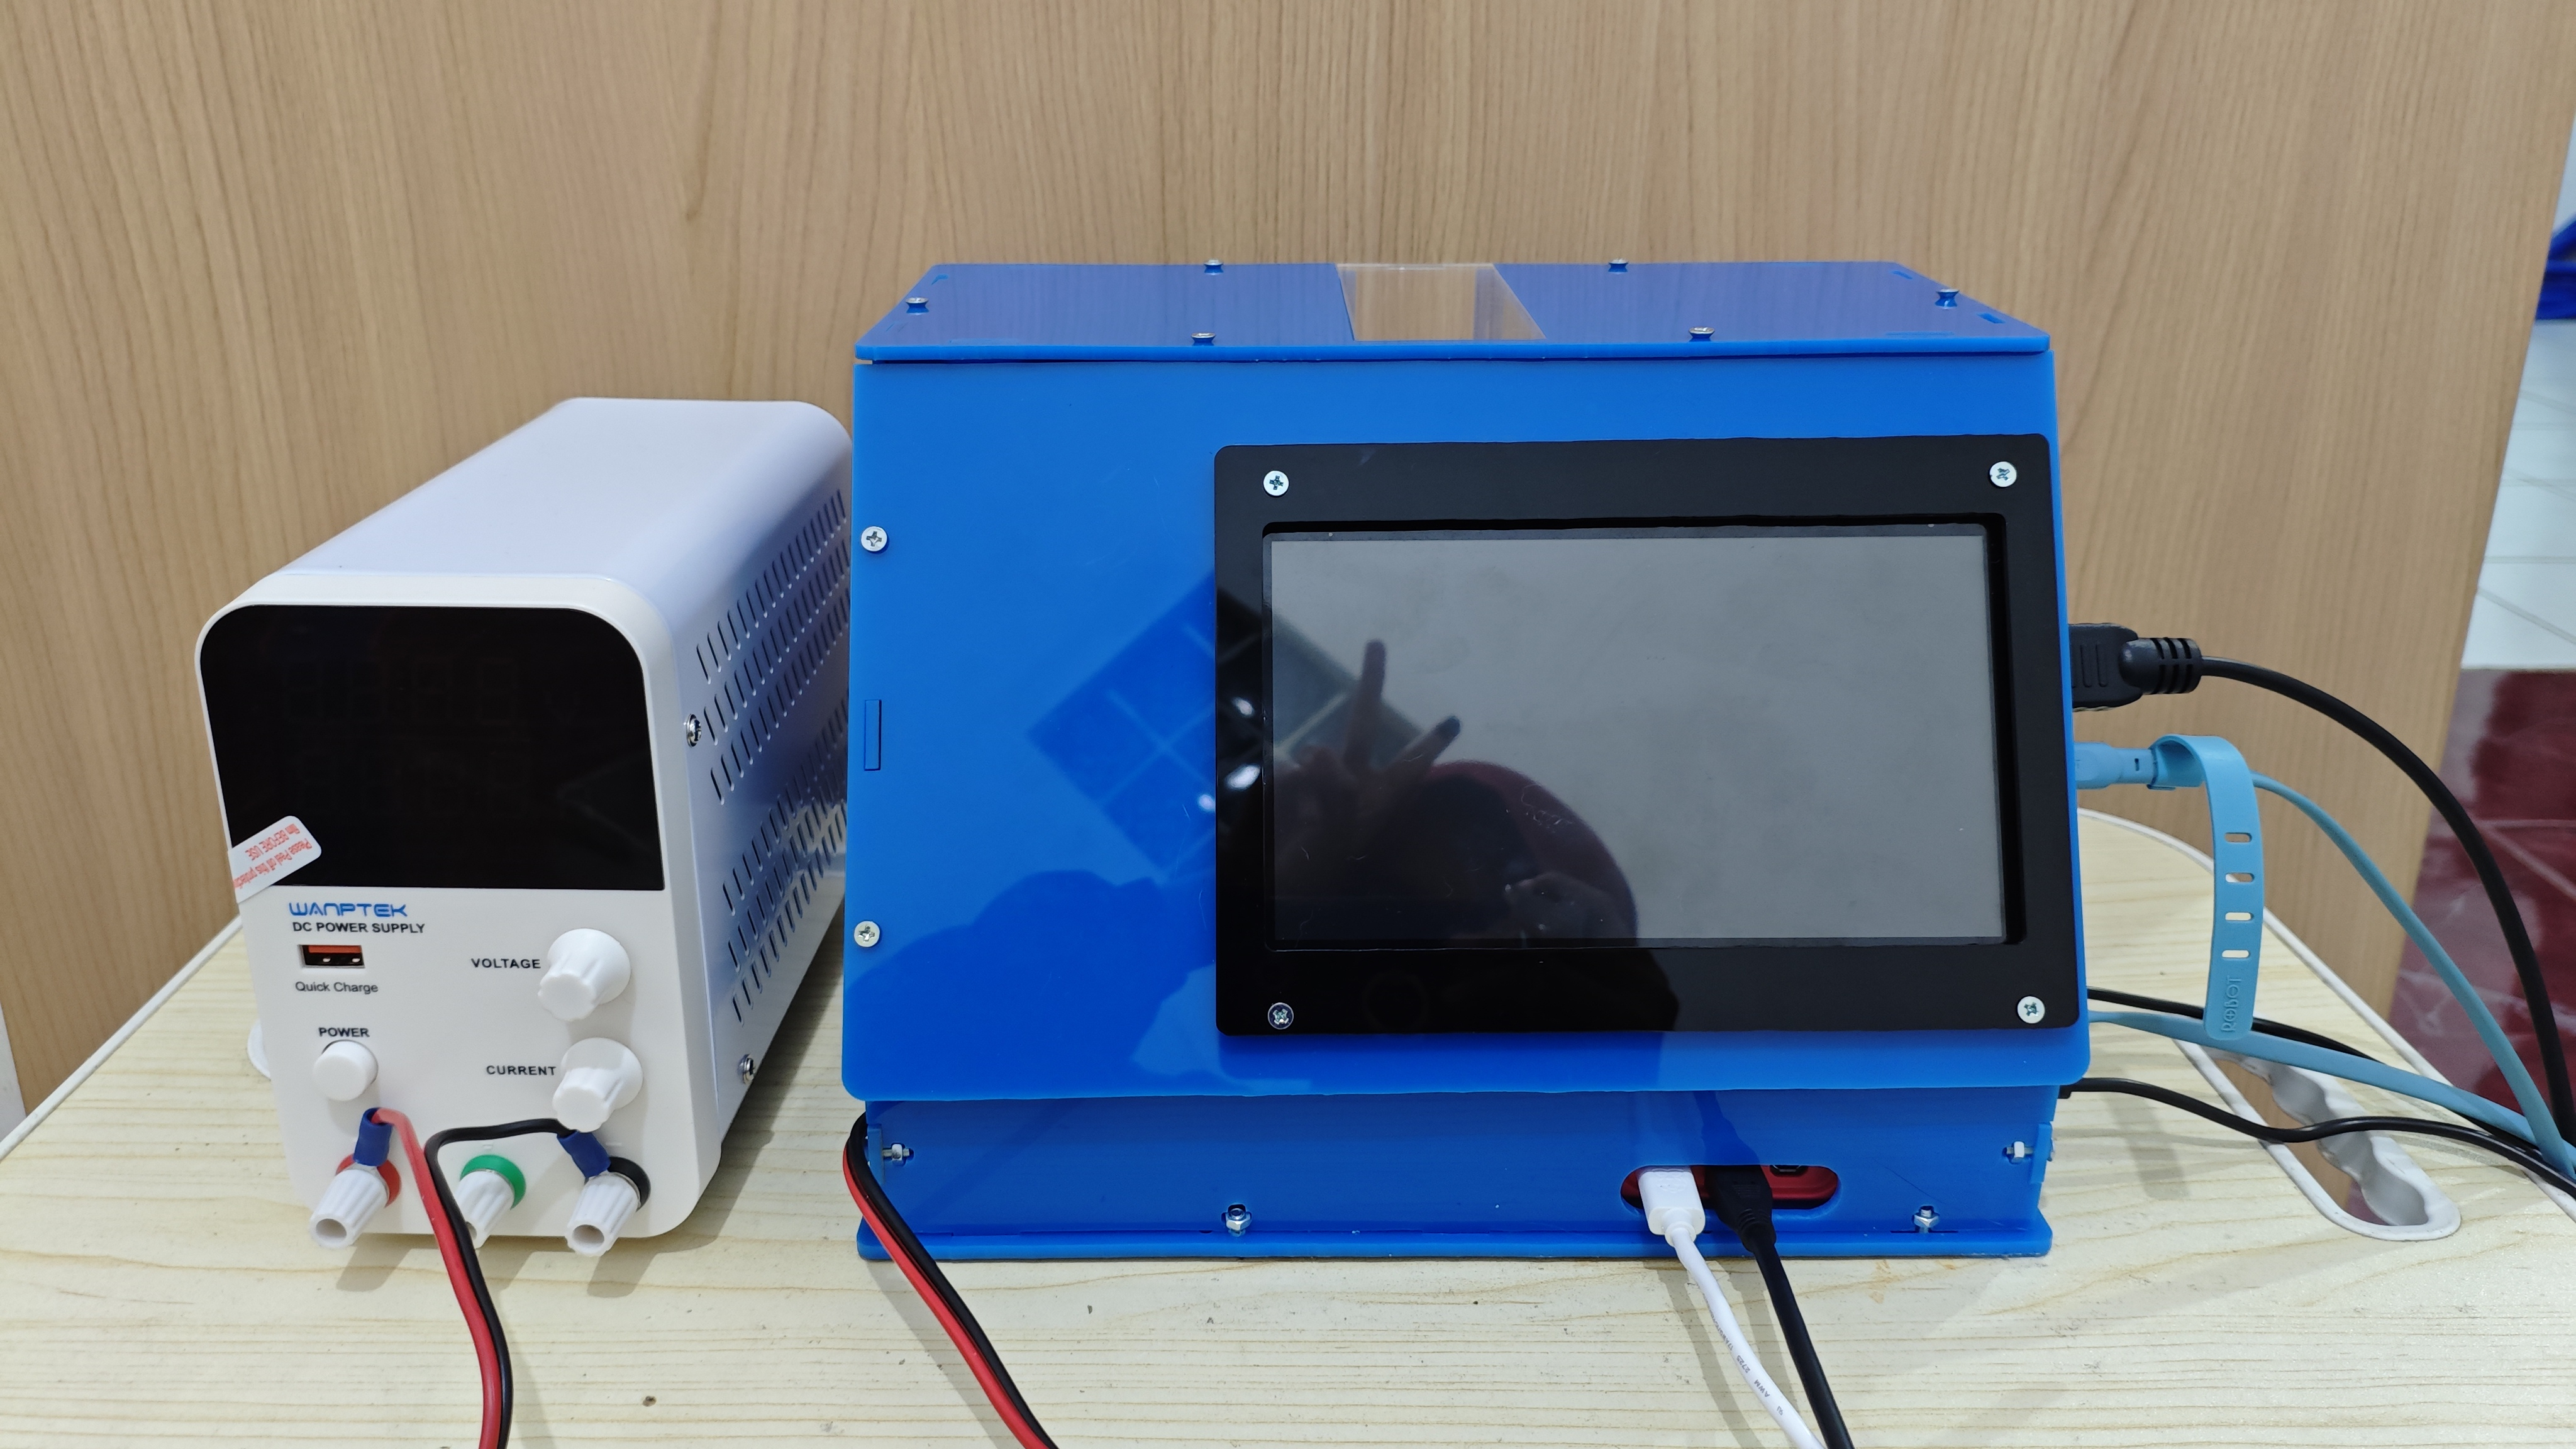
\includegraphics[width=\linewidth]{babIII_desainluar.jpg}
        \caption{Tampak Luar}
        \label{fig:realisasi_luar}
    \end{subfigure}
    \hfill
    \begin{subfigure}[b]{0.48\textwidth}
        \centering
        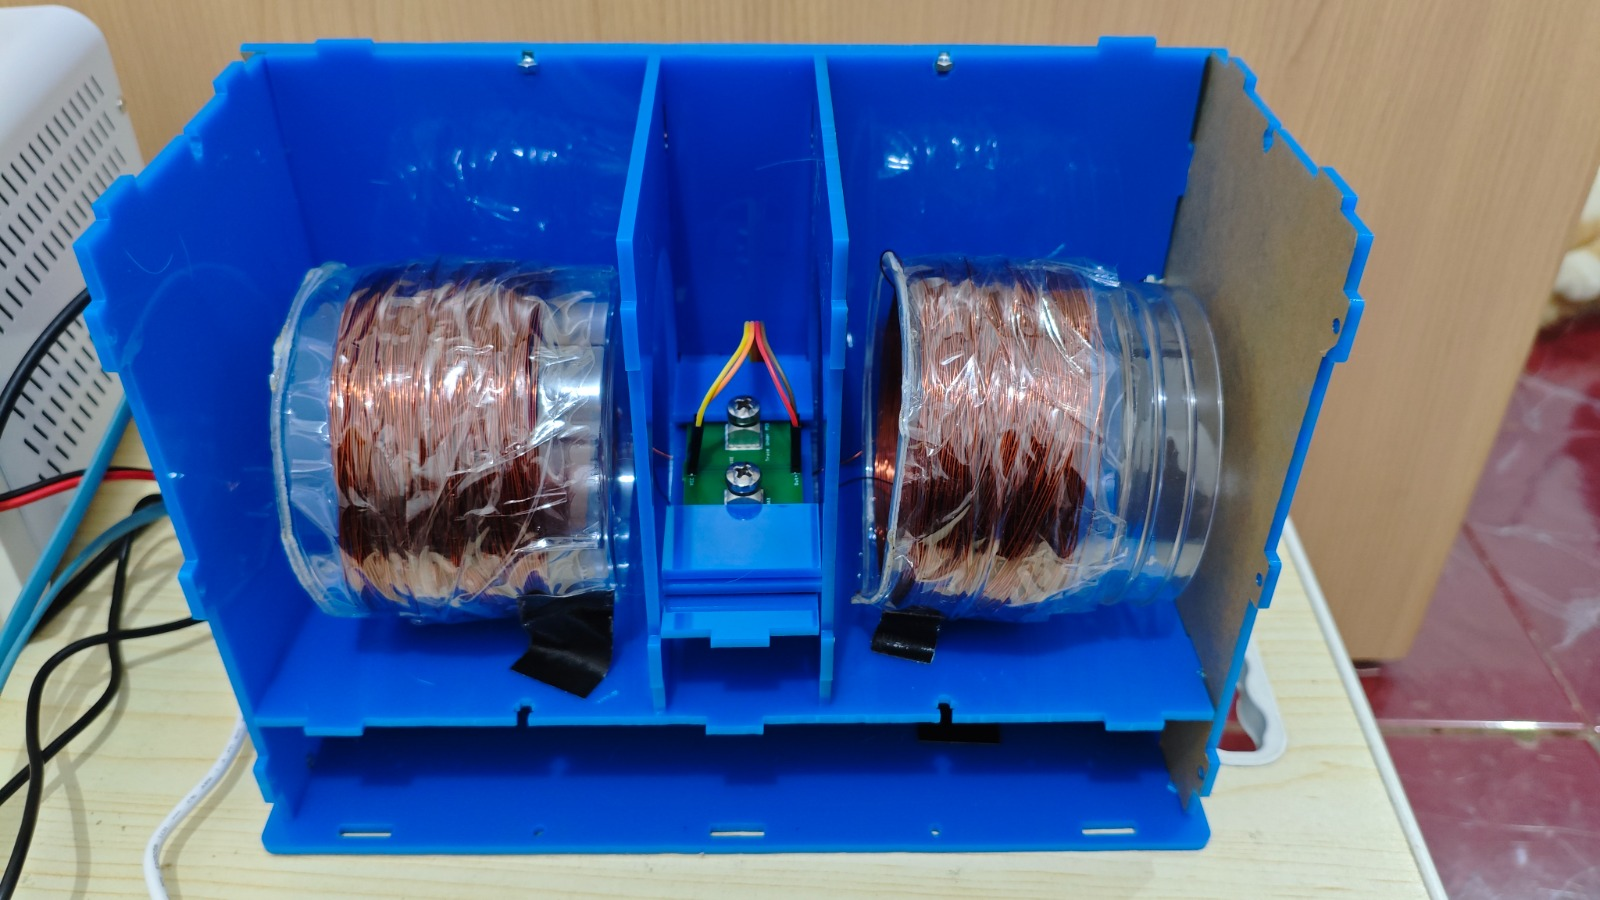
\includegraphics[width=\linewidth]{babIII_desaindalam.jpg}
        \caption{Tampak Dalam}
        \label{fig:realisasi_dalam}
    \end{subfigure}
    \caption{Realisasi Fisik Desain Mekatronika Kit Instrumentasi Sensor TMR}
    \label{fig:realisasi_casing}
\end{figure}

Sistem terintegrasi dari kit instrumentasi sensor TMR memuat berbagai komponen utama seperti mikrokomputer Raspberry Pi 5 beserta layar monitor terintegrasi, mikrokontroler Arduino Uno, papan sirkuit PCB instrumentasi sensor TMR, kumparan Helmholtz, sensor TMR ALT023-10E, hingga kabel penghubung terhadap catu daya eksternal.

\subsection{Perancangan Desain Rangkaian Perangkat Keras}
\begin{figure}[H]
    \centering
    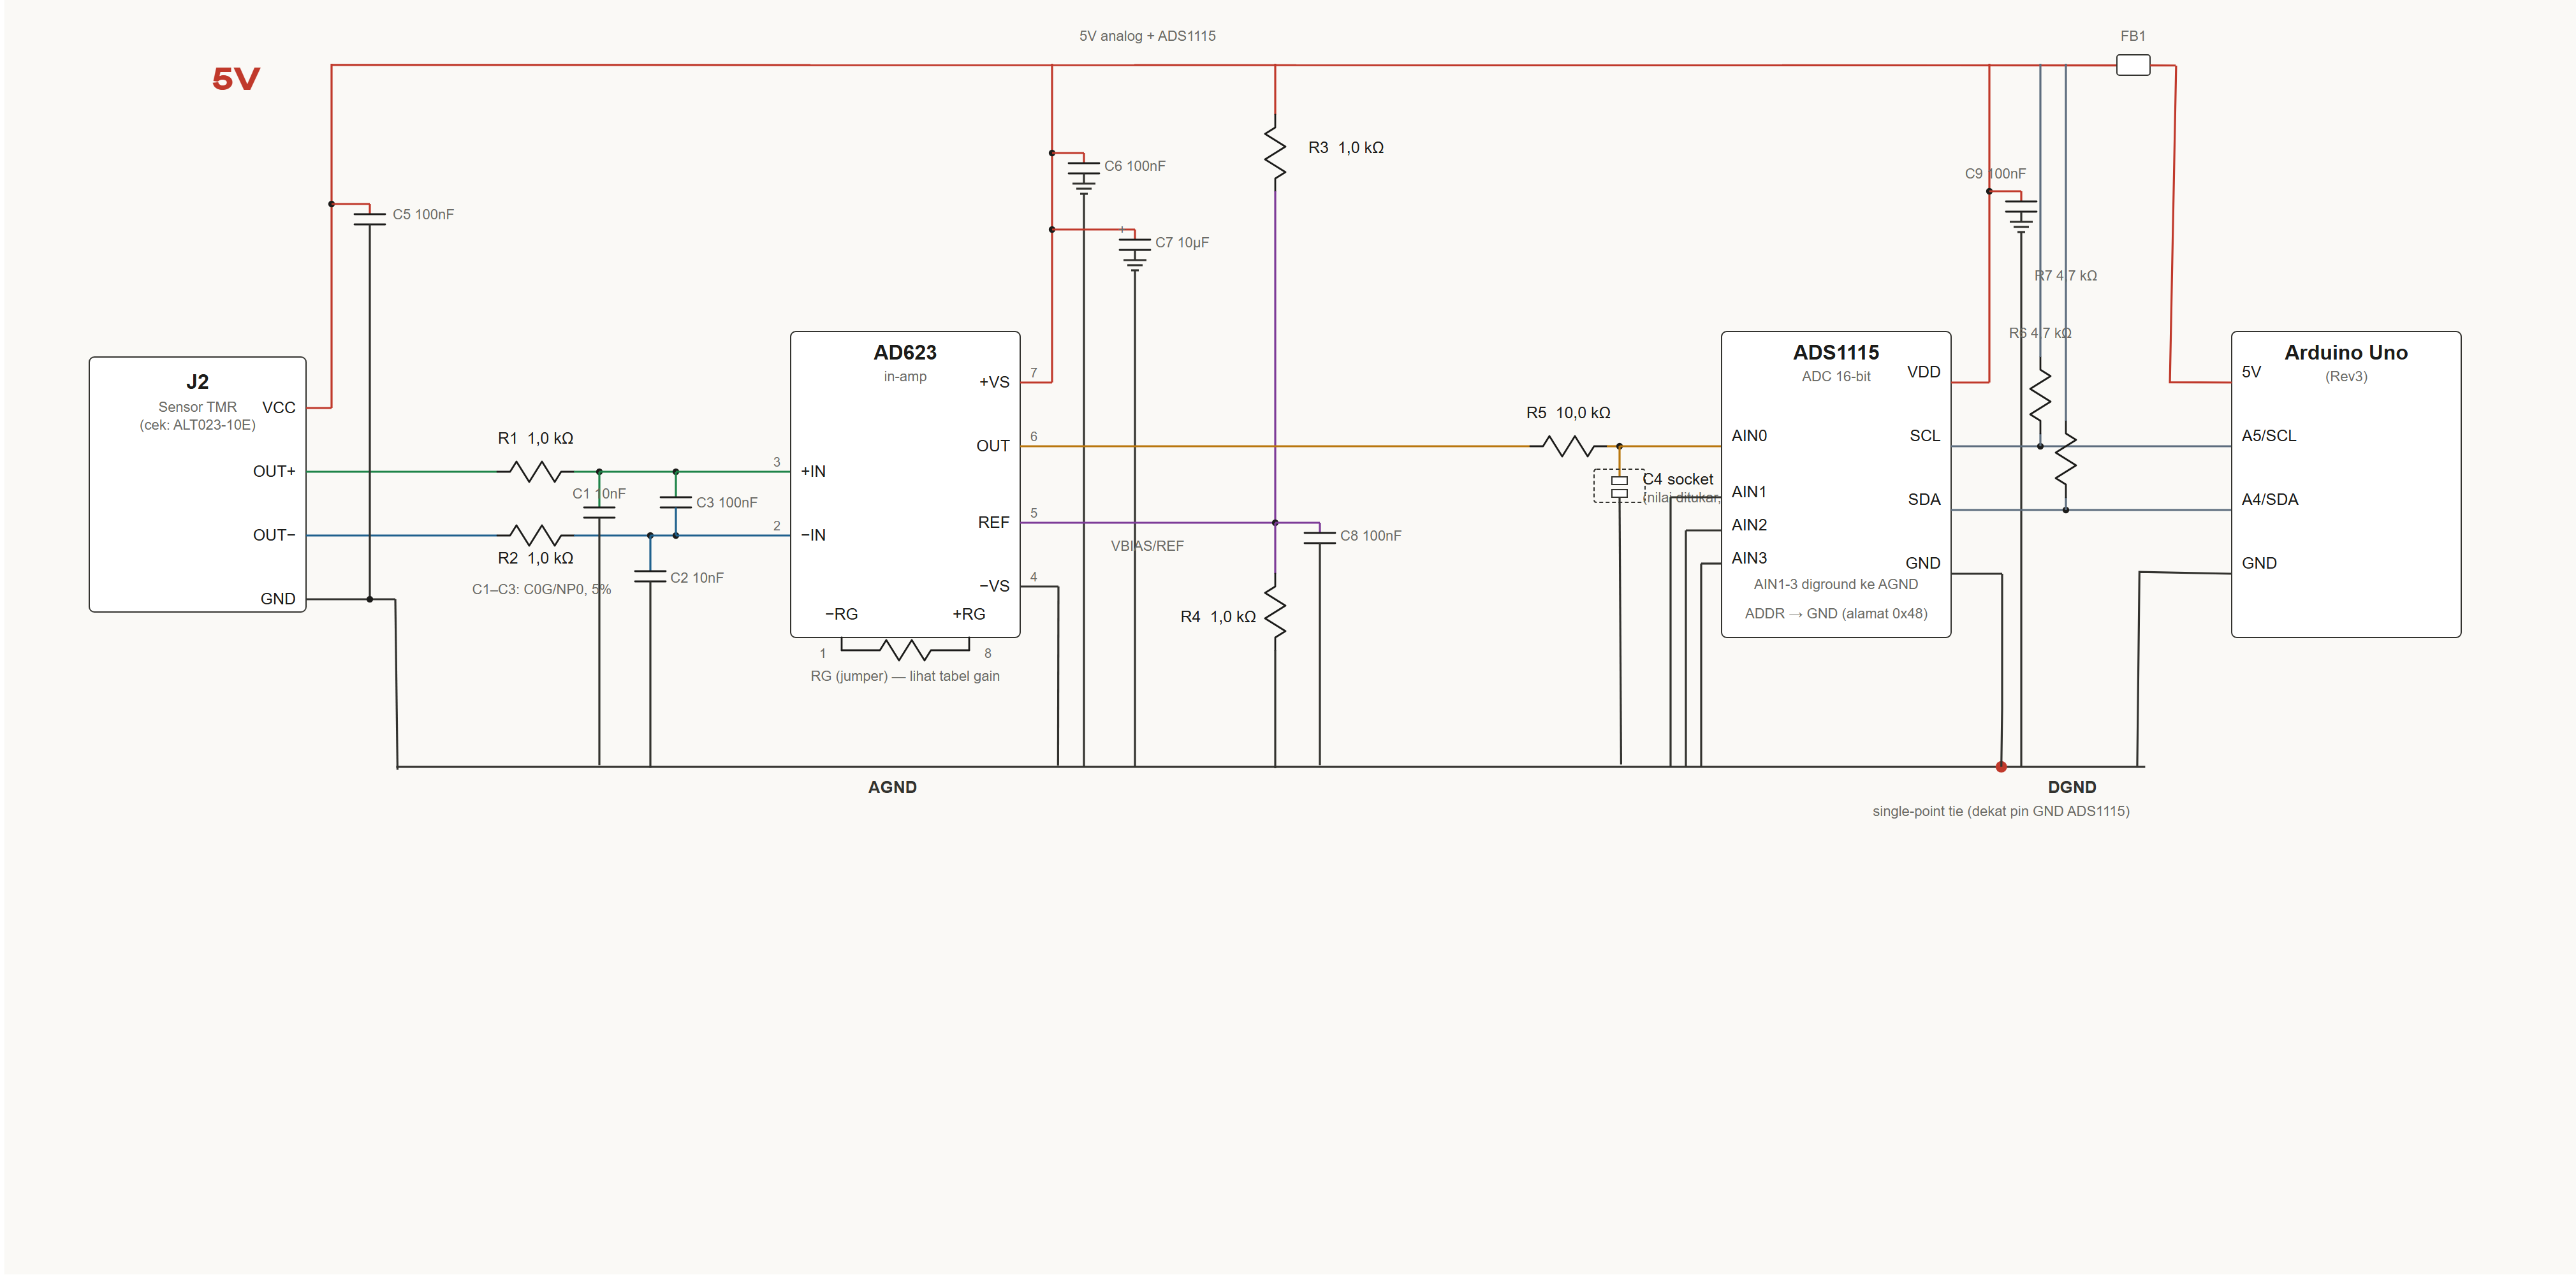
\includegraphics[width=1.0\linewidth]{babIII_skematik_TMR_grounding_fix.png}
    \caption{Desain Rangkaian Perangkat Keras Instrumentasi Sensor TMR ALT023-10E}
    \label{fig:skematik_hardware}
\end{figure}

Gambar~\ref{fig:skematik_hardware} menampilkan skema rangkaian perangkat keras kit instrumentasi sensor TMR ALT023-10E yang dirancang secara terintegrasi untuk mendeteksi perubahan medan magnet dan interaksi analit formalin. Rangkaian ini mengalirkan sinyal melalui rantai pengkondisian sinyal analog berpresisi tinggi hingga konversi digital:
\begin{enumerate}[label=\alph*)]
    \item \textbf{Unit Sensor TMR}: Menggunakan sensor analog TMR ALT023-10E dalam konfigurasi jembatan Wheatstone yang dicatu oleh tegangan 5~V dengan kapasitor \textit{decoupling} $C_5$ ($100\,\text{nF}$) untuk meredam fluktuasi suplai daya. Sensor menghasilkan tegangan diferensial bipolar ($OUT+$ dan $OUT-$) yang proporsional terhadap medan magnet terukur.
    \item \textbf{Filter RFI (\textit{Radio Frequency Interference})}: Sebelum masuk ke penguat instrumentasi, sinyal dari sensor dilewatkan melalui jaringan filter RFI yang tersusun dari resistor $R_1 = 1{,}0\,\text{k}\Omega$ dan $R_2 = 1{,}0\,\text{k}\Omega$, kapasitor diferensial $C_3 = 100\,\text{nF}$ (bertipe presisi C0G/NP0), serta dua kapasitor \textit{common-mode} $C_1 = 10\,\text{nF}$ dan $C_2 = 10\,\text{nF}$ ke ground. Filter ini berfungsi mencegah interferensi elektromagnetik dan sinyal frekuensi radio berorde megahertz memasuki tahap amplifikasi.
    \item \textbf{Penguat Instrumentasi (IC AD623)}: Sinyal diferensial yang telah tersaring dihubungkan ke masukan non-inverting (pin~3, $+IN$) dan inverting (pin~2, $-IN$) dari IC AD623. Penguatan (\textit{gain}) diatur menggunakan resistor gain eksternal presisi $R_G = 10{,}0\,\text{k}\Omega$ yang terpasang pada jumper antar-pin~1 dan pin~8 mengikuti persamaan $G = 1 + (100\,\text{k}\Omega / R_G) = 1 + (100 / 10) = 11$. Penguatan sebesar 11 kali ini memberikan rentang dinamik tegangan yang aman ($\pm 1{,}1\,\text{V}$) terhadap titik kerja $V_{\text{REF}} = 2{,}50\,\text{V}$ tanpa risiko kejenuhan (\textit{clipping}) pada rel catu daya 0--5 V. Guna mengakomodasi keluaran sensor bipolar pada sistem catu daya tunggal ($+V_S = 5\,\text{V}$, $-V_S = \text{AGND}$), pin referensi (\texttt{REF}, pin~5) dihubungkan ke titik tegangan bias $V_{BIAS} \approx 2{,}5\,\text{V}$ yang dibangkitkan melalui pembagi tegangan resistor $R_3 = 1{,}0\,\text{k}\Omega$ dan $R_4 = 1{,}0\,\text{k}\Omega$, serta distabilkan oleh kapasitor bypass $C_6 = 100\,\text{nF}$, $C_8 = 100\,\text{nF}$, dan kapasitor elektrolit $C_7 = 10\,\mu\text{F}$.
    \item \textbf{Filter Anti-Aliasing Pasif}: Keluaran dari pin~6 AD623 dilewatkan melalui filter \textit{low-pass} pasif RC yang terdiri atas resistor $R_5 = 10{,}0\,\text{k}\Omega$ dan kapasitor $C_4 = 100\,\text{nF}$ yang menghasilkan frekuensi potong $f_c \approx 159\,\text{Hz}$. Filter ini berfungsi membatasi lebar pita sinyal analog di bawah batas frekuensi Nyquist sebelum proses digitalisasi.
    \item \textbf{Konverter Analog ke Digital (ADC 16-bit ADS1115)}: Sinyal analog yang telah tersaring dihubungkan ke kanal masukan AIN0 ADS1115 secara \textit{single-ended}, sementara kanal AIN1 hingga AIN3 dihubungkan ke ground analog (AGND). Pin \texttt{ADDR} dihubungkan ke ground untuk menetapkan alamat I2C pada nilai default \texttt{0x48}. Penguat \textit{gain} internal (PGA) diatur pada rentang skala penuh $\pm 6{,}144\,\text{V}$ (\texttt{GAIN\_TWOTHIRDS}) agar seluruh dinamika tegangan 0--5~V keluaran AD623 dapat terakuisisi tanpa mengalami pemotongan (\textit{clipping}). Jalur komunikasi serial I2C (SDA dan SCL) dilengkapi resistor \textit{pull-up} $R_6 = 4{,}7\,\text{k}\Omega$ dan $R_7 = 4{,}7\,\text{k}\Omega$, serta kapasitor bypass $C_9 = 100\,\text{nF}$.
    \item \textbf{Mikrokontroler dan Manajemen Grounding}: Data digital 16-bit dibaca oleh Arduino Uno R3 melalui pin komunikasi I2C (A4/SDA dan A5/SCL). Guna mencegah injeksi derau penyaklaran digital (\textit{switching noise}) mikrokontroler ke dalam jalur pengukuran sensor berorde mikrovolt, rangkaian menerapkan pemisahan jalur ground analog (AGND) dan ground digital (DGND), yang disatukan hanya pada satu titik acuan bersama (\textit{single-point tie}) di dekat pin ground modul ADS1115.
\end{enumerate}

\subsection{Perancangan Perangkat Lunak}
\begin{figure}[H]
    \centering
    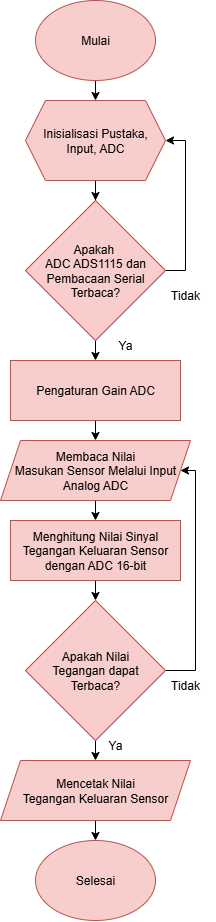
\includegraphics[width=0.33\textwidth]{babIII_AlurSoftwareArduino.drawio.png}
    \caption{Diagram Alir Pemrograman Perangkat Lunak Mikrokontroler}
    \label{fig:flowchart_arduino}
\end{figure}

Perancangan perangkat lunak pada penelitian ini dibagi menjadi dua bagian terintegrasi: perangkat lunak mikrokontroler (Arduino) untuk akuisisi streaming data mentah, dan perangkat lunak host (Python pada Raspberry Pi) untuk pengendalian kalibrasi, pengolahan statistik, serta pemodelan komparatif.

Alur pemrograman Arduino ditunjukkan pada Gambar~\ref{fig:flowchart_arduino}, yang diimplementasikan pada berkas kode \texttt{sensor\_tmr\_formalin.ino}. Program dimulai dari proses inisialisasi komunikasi serial pada kecepatan 115200 baud, serta inisialisasi antarmuka I2C melalui pustaka \texttt{Wire.h} dan \texttt{Adafruit\_ADS1X15.h}. Program melakukan deteksi ketersediaan modul ADS1115 pada alamat \texttt{0x48}; jika tidak terdeteksi, sistem menampilkan pesan kesalahan dan berhenti. Setelah berhasil terdeteksi, PGA diatur pada \texttt{GAIN\_TWOTHIRDS} ($\pm 6{,}144\,\text{V}$) dan laju konversi diatur pada \texttt{RATE\_ADS1115\_128SPS} (sekitar 1 baris data per 7,8 ms). Pada loop utama, program membaca sinyal analog dari pin AIN0 secara \textit{single-ended}, mengonversinya menjadi nilai tegangan melalui fungsi \texttt{computeVolts()} dan formula LSB manual ($V_{FSR}/32768$), serta menerima label konsentrasi analit secara dinamis melalui antarmuka serial. Seluruh data mentah dialirkan secara kontinu dalam format CSV (\texttt{millis}, \texttt{label}, \texttt{raw\_adc}, \texttt{tegangan\_lib\_V}, \texttt{tegangan\_manual\_V}) tanpa operasi rata-rata pada Arduino, sehingga mikrokontroler tetap ringan dan responsif.

\begin{figure}[H]
    \centering
    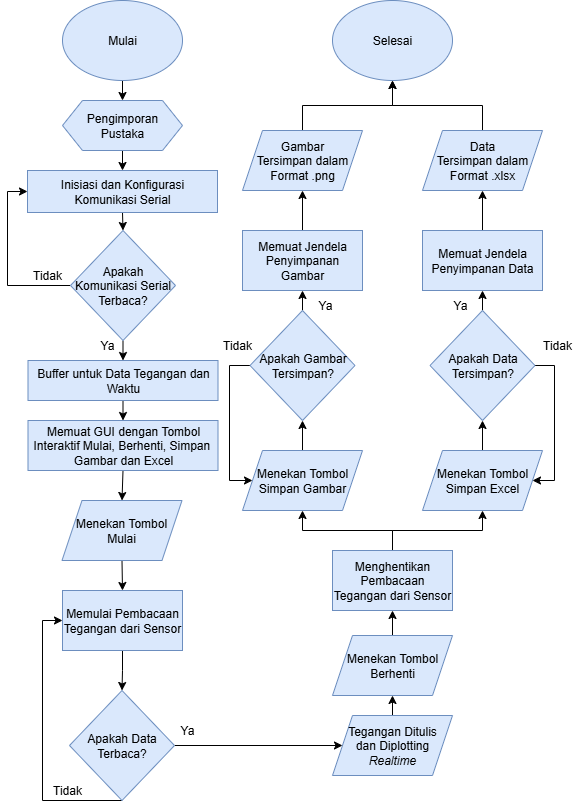
\includegraphics[width=0.85\textwidth]{babIII_DiagramAlirPython.drawio.png}
    \caption{Diagram Alir Pemrograman Perangkat Lunak Python}
    \label{fig:flowchart_python}
\end{figure}

Alur pemrograman Python pada Raspberry Pi ditunjukkan pada Gambar~\ref{fig:flowchart_python}, yang diimplementasikan pada skrip \texttt{kalibrasi\_tmr\_formalin.py}. Skrip ini memanfaatkan pustaka \texttt{serial}, \texttt{numpy}, dan \texttt{matplotlib}. Prosedur akuisisi dan pemodelan berjalan sebagai berikut:
\begin{enumerate}
    \item Membuka port komunikasi serial ke Arduino pada baud rate 115200 dan mengosongkan buffer serial setelah jeda reset mikrokontroler.
    \item Pengguna memasukkan deretan konsentrasi formalin standar yang diuji (mg/L).
    \item Pada setiap titik konsentrasi:
    \begin{itemize}
        \item Program mengirimkan label konsentrasi ke Arduino agar tercatat pada setiap baris data mentah.
        \item Setelah sensor dicelupkan ke larutan uji, sistem akuisisi \texttt{DurationAcquisitionEngine} melakukan perekaman berbasis durasi waktu (5.0 detik) dan mengabaikan data transien 1.0 detik pertama (\textit{settling time}) untuk membuang efek transien.
        \item Sistem mengumpulkan sampel tegangan kondisi tunak selama durasi stabil 4.0 detik berikutnya, kemudian menghitung nilai rata-rata dan simpangan baku tegangan untuk titik tersebut.
    \end{itemize}
    \item Setelah seluruh variasi konsentrasi selesai diakuisisi, program secara otomatis menghitung kurva kalibrasi melalui regresi linear kuadrat terkecil, menghasilkan persamaan regresi $V = m \cdot C + c$, koefisien determinasi ($R^2$), sensitivitas sensor ($m = \Delta V / \Delta C$), serta batas deteksi (\textit{Limit of Detection}, LOD).
    \item Hasil pengujian disimpan ke dalam berkas \texttt{data\_mentah\_\allowbreak kalibrasi.csv} (seluruh sampel per milidetik), \texttt{ringkasan\_\allowbreak kalibrasi.csv} (titik rata-rata dan stdev), serta visualisasi grafik kurva kalibrasi berstandar publikasi dalam format PNG.
\end{enumerate}

\begin{figure}[H]
    \centering
    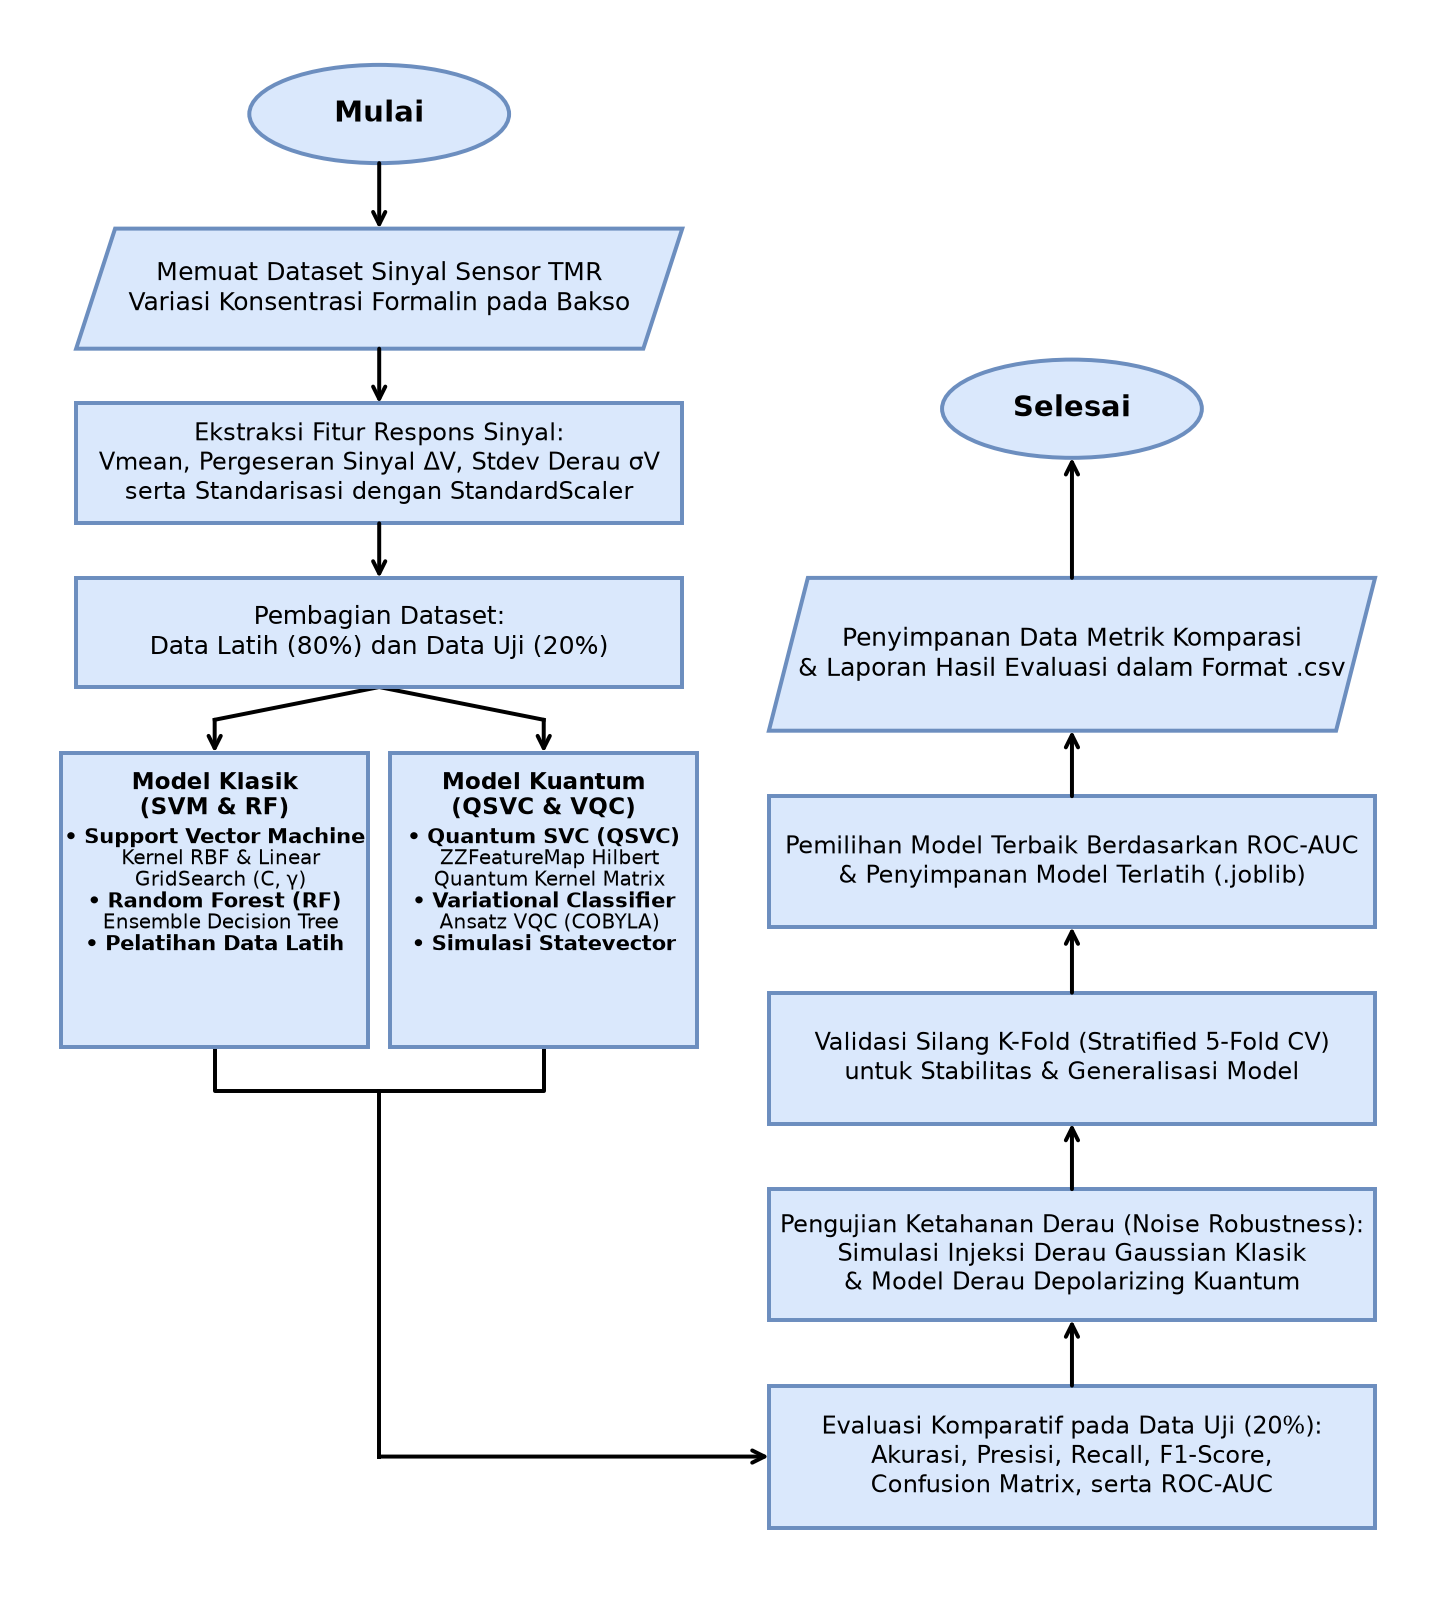
\includegraphics[width=0.80\textwidth]{babIII_ModelBuilding.drawio.png}
    \caption{Diagram Alir Pembuatan, Pelatihan, dan Komparasi Model Klasifikasi (Model Klasik: SVM, RF vs. Model Kuantum: QSVC, VQC)}
    \label{fig:flowchart_model_building}
\end{figure}

Gambar~\ref{fig:flowchart_model_building} menunjukkan alur pelatihan dan komparasi model \textit{machine learning} yang digunakan untuk mengklasifikasikan konsentrasi formalin berdasarkan fitur sinyal sensor TMR. Dataset yang digunakan merupakan kumpulan fitur yang diekstraksi dari pengujian variasi konsentrasi formalin standar ($V_{\text{mean}}$, $\Delta V$, $\sigma_V$). Data distandardisasi menggunakan \texttt{StandardScaler} dan dibagi menjadi set pelatihan (80\%) dan set pengujian (20\%). Dua paradigma dilatih dan dibandingkan secara paralel: dua model klasik, yaitu \textit{Support Vector Machine} (SVM) dengan optimasi hyperparameter $C$ dan $\gamma$ serta \textit{Random Forest} (RF) dengan optimasi jumlah pohon (\textit{n\_estimators}) dan kedalaman (\textit{max\_depth}); serta dua model kuantum, yaitu \textit{Quantum Support Vector Classifier} (QSVC) berbasis pemetaan ruang Hilbert (\textit{ZZFeatureMap}) dan komputasi \textit{Quantum Kernel Matrix} ($K_Q$), serta \textit{Variational Quantum Classifier} (VQC) berbasis sirkuit kuantum variasional parametrik. Evaluasi performa dilakukan secara komparatif melalui \textit{stratified 5-fold cross-validation} dengan metrik akurasi, presisi, \textit{recall}, \textit{F1-score}, \textit{confusion matrix}, ROC-AUC, waktu komputasi, serta evaluasi ketahanan model terhadap injeksi derau (\textit{noise robustness}) baik derau Gaussian klasik maupun model derau kuantum depolarizing. Model terbaik yang menghasilkan generalisasi tertinggi kemudian disimpan untuk tahap penerapan (\textit{deployment}).

\begin{figure}[H]
    \centering
    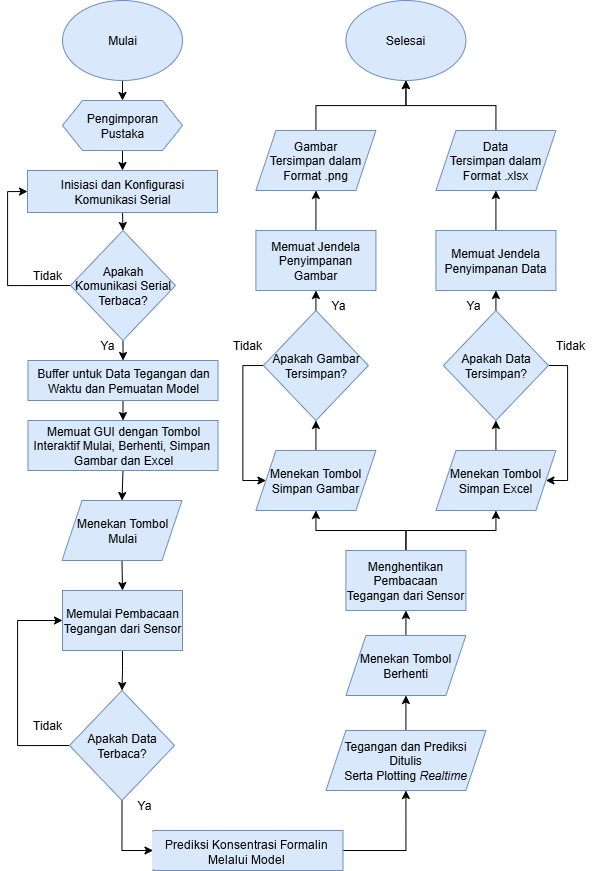
\includegraphics[width=0.85\textwidth]{babIII_ModelDeploy.drawio.png}
    \caption{Diagram Alir \textit{Deployment} Model}
    \label{fig:flowchart_model_deploy}
\end{figure}

Gambar~\ref{fig:flowchart_model_deploy} menggambarkan alur penerapan model yang telah dilatih untuk deteksi dan klasifikasi konsentrasi formalin pada bakso secara \textit{realtime}. Sistem berjalan pada perangkat komputer papan tunggal Raspberry Pi 5 yang terintegrasi dengan layar sentuh interaktif. Ketika ekstrak sampel bakso diteteskan ke atas membran nanofiber sensor TMR, data tegangan dialirkan secara kontinu oleh Arduino Uno. Program Python melakukan penangkapan jendela sinyal tunak sebanyak 500 sampel, mengekstraksi vektor fiturnya, lalu melakukan inferensi menggunakan model terbaik. Hasil prediksi berupa status keamanan pangan (Aman / Bebas Formalin vs Berbahaya / Mengandung Formalin) beserta estimasi kadar analit ditampilkan langsung pada antarmuka grafis (\textit{GUI}) interaktif dan dicatat ke dalam basis data log pengujian.

\subsection{Tahapan Sintesis Sampel Uji}
Tahapan sintesis dan preparasi sampel uji ditunjukkan secara sistematis pada Gambar~\ref{fig:diagram_alir_sintesis}, yang melingkupi seluruh rangkaian mulai dari sintesis prekursor, dispersi sitrat, elektrospinning, hingga penautan silang dan fungsionalisasi reseptor.

\begin{figure}[H]
    \centering
    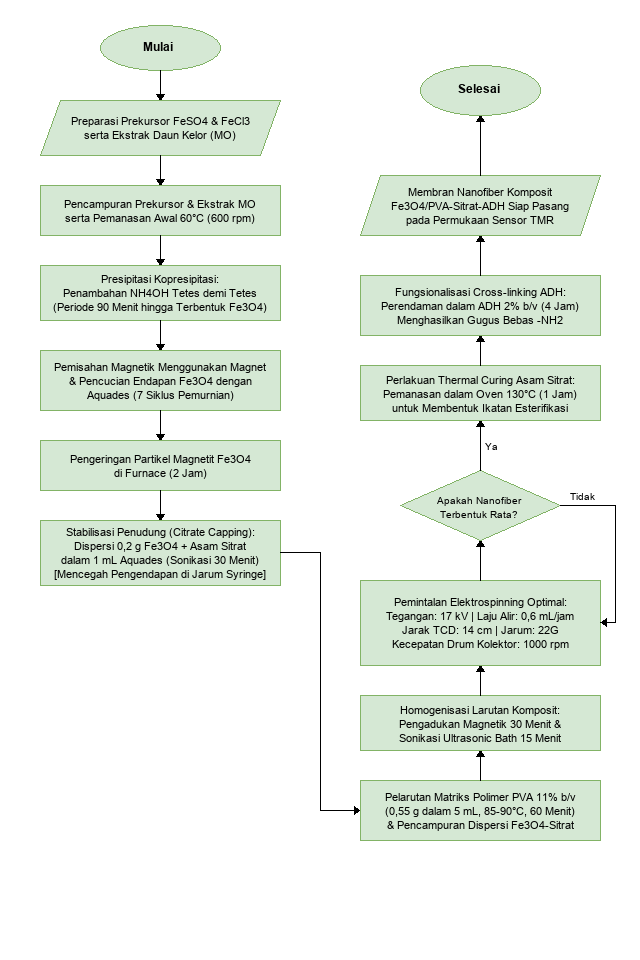
\includegraphics[width=0.82\textwidth]{babIII_DiagramAlirSintesis.drawio.png}
    \caption{Diagram Alir Sintesis dan Fabrikasi Nanofiber Komposit \ch{Fe3O4}/PVA-Sitrat-ADH}
    \label{fig:diagram_alir_sintesis}
\end{figure}

\subsubsection{Sintesis Nanopartikel Magnetik \ch{Fe3O4}}
Sintesis nanopartikel magnetik \ch{Fe3O4} dimulai dengan persiapan dua larutan prekursor besi yang dipisah: larutan \ch{FeSO4} sebanyak \SI{7.5}{mL} dan larutan \ch{FeCl3} sebanyak \SI{7.5}{mL}. Masing-masing larutan prekursor diaduk sendiri-sendiri selama \SI{15}{menit} pada kecepatan pengadukan \SI{600}{rpm} pada suhu kamar sekitar \SI{22}{\degree C} untuk memastikan homogenitas larutan dan melarutkan garam besi secara penuh. Setelah periode pengadukan awal selesai, kedua larutan prekursor digabungkan dan proses pengadukan dilanjutkan sambil dilakukan pemanasan awal untuk menaikkan suhu campuran hingga \SI{60}{\degree C}; selama kenaikan suhu ini kecepatan pengadukan dikurangi dan dikontrol pada kisaran \SI{480}--\SI{550}{rpm} untuk meminimalkan percikan dan memastikan transfer panas yang seragam.

Pemanasan berlanjut secara bertahap sampai suhu campuran mencapai puncak sementara \SI{107}{\degree C} (nilai maksimal yang dicapai selama pemanasan bertahap), lalu suhu diturunkan dan distabilkan pada \SI{60}{\degree C}. Dalam fase ini, suhu dipertahankan stabil selama \SI{15}{menit} sambil secara aktif mengontrol profil pendinginan sehingga suhu campuran mengalami penurunan terkontrol ke kisaran \SI{100}--\SI{102}{\degree C} secara berkala; tahapan ini bertujuan mengatur kinetika reaksi awal pembentukan inti (\textit{nucleation}) dan pertumbuhan butir (\textit{growth}) agar ukuran partikel dapat dikontrol secara presisi.

Setelah fase stabilisasi awal selesai, ditambahkan ekstrak \textit{Moringa oleifera} (MO) sebanyak \SI{10}{mL} ke dalam campuran. Ekstrak MO berfungsi sebagai agen pereduksi dan agen penstabil permukaan melalui gugus hidroksil ($-\text{OH}$) dan senyawa polifenolik yang hadir di dalamnya; gugus-gugus ini dapat berperan dalam mengikat permukaan partikel besi yang terbentuk, menghambat aglomerasi, serta membantu mengontrol laju reduksi ion besi sehingga pembentukan fase magnetit (\ch{Fe3O4}) berjalan lebih terkendali. Setelah penambahan MO, campuran terus diaduk pada suhu terkontrol \SI{60}{\degree C} selama \SI{30}{menit} dengan fluktuasi suhu yang dikendalikan sehingga kondisi suhu tetap stabil namun memungkinkan pertukaran energi yang diperlukan untuk transformasi kimia dan rekristalisasi permukaan partikel.

Selanjutnya, disiapkan larutan basa amonia (\ch{NH4OH}) sebagai sumber ion hidroksida untuk memicu presipitasi dan pembentukan fase oksida magnetik. Larutan amonia dibuat dengan mencampurkan \SI{12}{mL} \ch{NH4OH} pekat dengan \SI{18}{mL} air deionisasi (akuades) dan diaduk selama \SI{12}{menit} pada kecepatan pengadukan \SI{450}{rpm} pada suhu stabil sekitar \SI{27}{\degree C} untuk memperoleh larutan amonia yang homogen. Larutan amonia ini kemudian ditambahkan ke dalam campuran prekursor-MO secara tetes demi tetes sepanjang periode \SI{90}{menit} dengan pengadukan kontinu. Penambahan secara perlahan ini dilakukan untuk mengendalikan pH lokal dan laju presipitasi sehingga pembentukan partikel tidak berlangsung terlalu cepat (mencegah terbentuknya partikel kasar dan aglomerasi) serta menjaga distribusi ukuran partikel tetap sempit.

Selama penambahan amonia dan fase stabilisasi, pengadukan dipertahankan untuk memastikan pencampuran dan difusi ion yang baik antar fase. Setelah seluruh amonia ditambahkan dan sistem mengalami stabilisasi partikel, campuran didinginkan hingga mencapai suhu sekitar \SI{35}{\degree C} untuk menghentikan reaksi atau memperlambat laju pertumbuhan partikel. Pada tahap pemurnian, nanopartikel magnetik yang terbentuk dipisahkan dari fase cair menggunakan magnet permanen yang ditempatkan di bawah wadah selama \SI{15}{menit}; medan magnet menyebabkan endapan magnetit beragregasi di dinding wadah yang berdekatan dengan magnet sehingga supernatan (fase cair) dapat dituangkan atau disingkirkan tanpa kehilangan endapan.

Pencucian endapan dilakukan menggunakan akuades dan diulang sebanyak tujuh siklus untuk menghilangkan ion sisa, garam terlarut, residu organik dari ekstrak MO, dan pengotor lainnya. Setiap siklus pencucian umumnya meliputi penambahan volume akuades yang sesuai, pengadukan singkat untuk melarutkan pengotor, pemisahan magnetik, pembuangan supernatan, dan pengulangan sampai tujuh kali sehingga konduktivitas atau kejernihan supernatan menunjukkan kemurnian yang diinginkan. Setelah pencucian akhir, endapan magnetit dikumpulkan dan dikeringkan di dalam oven pengering pada kondisi yang ditentukan selama \SI{2}{jam} untuk menghilangkan kelembapan tersisa dan memadatkan butiran nanopartikel; suhu pengeringan akhir sebaiknya disesuaikan dengan kebutuhan sifat magnetik dan termal.

\subsubsection{Preparasi Larutan Matriks PVA dan Dispersi \texorpdfstring{\ch{Fe3O4}}{Fe3O4} Terstabilisasi Asam Sitrat}
Tahap preparasi material diawali secara bertahap dari penyiapan larutan matriks polimer \textit{polyvinyl alcohol} (PVA) dan stabilisasi nanopartikel magnetik \ch{Fe3O4}:
\begin{enumerate}
    \item \textbf{Preparasi Larutan Matriks PVA}: PVA ditimbang sebanyak \SI{0.55}{g} (menghasilkan konsentrasi sekitar 11\% b/v dalam \SI{5}{mL} akuades). Akuades dimasukkan ke dalam vial kaca dan dipanaskan di atas \textit{magnetic stirrer} hingga mencapai suhu \SI{60}{\degree C}. Serbuk PVA dimasukkan perlahan ke dalam vial sambil diaduk pada kecepatan \SI{600}{rpm}. Pemanasan dilanjutkan hingga suhu larutan mencapai \SI{85}--\SI{90}{\degree C}, dan dijaga konstan selama \SI{60}{menit} hingga seluruh butiran PVA terlarut sempurna membentuk larutan kental bening yang homogen. Peningkatan konsentrasi PVA dari 9\% menjadi 11\% bertujuan meningkatkan derajat belitan rantai polimer (\textit{chain entanglement}) dan viskoelastisitas larutan, sehingga mampu menjebak dan menyeret nanopartikel besi ke dalam jet elektrospinning tanpa putus. Larutan kemudian didinginkan secara bertahap hingga mencapai suhu ruang.
    \item \textbf{Dispersi dan Stabilisasi Partikel \ch{Fe3O4} dengan Asam Sitrat}: Sebanyak \SI{0.2}{g} nanopartikel \ch{Fe3O4} hasil sintesis kopresipitasi ditimbang dan dimasukkan ke dalam \SI{1}{mL} akuades yang telah ditambahkan asam sitrat pro-analisis sebagai agen penudung (\textit{capping agent}). Campuran disonikasi menggunakan \textit{ultrasonic bath} selama \SI{30}{menit} pada suhu ruang. Berdasarkan hasil evaluasi awal menggunakan \textit{Scanning Electron Microscopy} (SEM) pada formula terdahulu, ketiadaan agen penstabil menyebabkan nanopartikel \ch{Fe3O4} menggumpal secara cepat akibat gaya tarik dipol magnetik dan mengalami sedimentasi gravitasi di dasar tabung jarum suntik selama operasi pemintalan berjam-jam, sehingga kandungan \ch{Fe3O4} pada lembaran nanofiber terdeteksi nyaris nol. Penambahan asam sitrat menghasilkan lapisan koordinasi karboksilat ($- \text{COO}^-$) pada permukaan kation besi partikel magnetit, memberikan potensial zeta negatif tinggi yang membangkitkan gaya tolak elektrostatik dominan. Stabilisasi ini menjamin nanopartikel \ch{Fe3O4} terdispersi stabil dan tidak mengendap di dalam jarum suntik.
    \item \textbf{Pencampuran Homogen}: Dispersi \ch{Fe3O4}-Sitrat dituangkan ke dalam larutan PVA 11\%, kemudian diaduk dengan \textit{magnetic stirrer} selama \SI{30}{menit} dan disonikasi kembali selama \SI{15}{menit} untuk memastikan dispersi nanopartikel terdistribusi seragam di seluruh jejaring larutan polimer sebelum proses pemintalan.
\end{enumerate}

\subsubsection{Fabrikasi Nanofiber Komposit melalui Elektrospinning dan Optimasi Parameter}
Fabrikasi lembaran nanofiber dilakukan menggunakan perangkat \textit{electrospinning} dengan sabuk penggerak pompa presisi. Kelembapan relatif di dalam ruang kerja alat diatur pada kisaran 45--50\% menggunakan tabung silika gel guna memastikan laju penguapan pelarut yang stabil. Larutan komposit \ch{Fe3O4}/PVA-Sitrat dimasukkan ke dalam jarum suntik 5~mL yang dilengkapi jarum berujung tumpul (\textit{blunt needle}) ukuran 22G. Sebagai media kolektor, lembaran aluminium foil ($20 \times 10\,\text{cm}$) direkatkan pada permukaan drum kolektor putar.

Parameter operasional elektrospinning diatur pada nilai optimal berdasarkan kajian reologi dan fenomena elektrohidrodinamika:
\begin{itemize}
    \item \textbf{Tegangan Tinggi (\textit{Applied Voltage})}: Diatur pada rentang optimal 16--18~kV (dengan titik kerja utama \SI{17}{kV}). Kuat medan listrik ini menghasilkan gaya elektrostatik yang cukup kuat untuk mengatasi tegangan permukaan larutan komposit kental dan membentuk \textit{Taylor cone} yang stabil tanpa fluktuasi.
    \item \textbf{Laju Alir (\textit{Flow Rate})}: Diatur pada rentang \SI{0.4}--\SI{0.8}{mL/jam} (setara dengan \SI{7}--\SI{13}{\micro L/min}, dengan titik kerja utama \SI{0.6}{mL/jam} atau \SI{10}{\micro L/min}). Laju alir ini diturunkan secara terukur dari parameter lama (\SI{15}{\micro L/min}) guna mencegah pembentukan tetesan berlebih (\textit{dripping}) dan memastikan pelarut menguap sempurna selama waktu terbang jet.
    \item \textbf{Jarak Ujung Jarum ke Kolektor (\textit{Tip-to-Collector Distance}, TCD)}: Ditetapkan pada jarak \SI{14}{cm} (rentang 13--15~cm) untuk memberikan waktu terbang dan peregangan jet (\textit{whipping instability}) yang cukup sehingga menghasilkan serat berdiameter seragam tanpa cacat butiran (\textit{bead-free}).
    \item \textbf{Kecepatan Kolektor dan Durasi}: Kolektor drum diputar pada kecepatan konstan \SI{1000}{rpm} selama 2--3 jam hingga terbentuk lapisan nanofiber tipis berwarna kecokelatan merata pada aluminium foil.
\end{itemize}
Validasi keseragaman morfologi dan keberadaan nanopartikel besi ditempuh melalui perancangan variasi optimasi bertingkat (tegangan 15, 17, dan 19~kV serta laju alir 8, 10, dan 12~$\mu$L/min) yang dikarakterisasi menggunakan SEM dan \textit{Energy-Dispersive X-ray Spectroscopy} (EDX) guna mengonfirmasi distribusi spasial unsur besi (Fe) pada lembaran nanofiber.

\subsubsection{Penautan Silang Termal Asam Sitrat dan Fungsionalisasi ADH}
Lembaran nanofiber komposit yang diperoleh selanjutnya menjalani perlakuan pasca-fabrikasi (\textit{post-treatment}) bertahap:
\begin{enumerate}
    \item \textbf{Penautan Silang Termal (\textit{Thermal Curing})}: Lembaran nanofiber komposit dipanaskan di dalam oven pengering pada suhu $130\,^{\circ}\text{C}$ selama 1,5 jam untuk mengaktivasi reaksi esterifikasi antara gugus karboksil asam sitrat dan gugus hidroksil PVA, membentuk jejaring ikatan ester kovalen antar-rantai polimer. Proses ini menjadikan nanofiber bersifat tahan air (\textit{water-insoluble}), mencegah degradasi serat saat dibasahi larutan uji, serta mempertahankan partikel \ch{Fe3O4} tertanam kokoh di dalam matriks serat.
    \item \textbf{Fungsionalisasi Gugus Reseptor ADH}: Lembaran nanofiber yang telah tertaut silang kemudian direndam ke dalam larutan \textit{adipic acid dihydrazide} (ADH) 2\% (b/v) dalam akuades selama \SI{30}{menit}, lalu dibilas dengan akuades untuk menghilangkan kelebihan ADH yang tidak terikat dan dikeringkan pada suhu ruang. Gugus hidrazida terminal ($- \text{CO}-\text{NH}-\text{NH}_2$) dari ADH yang tertambat pada permukaan nanofiber bertindak sebagai reseptor molekuler (\textit{chemo-receptor}) selektif terhadap molekul formaldehida bebas melalui pembentukan ikatan kovalen hidrazon.
\end{enumerate}
Lembaran nanofiber komposit \ch{Fe3O4}/PVA-Sitrat-ADH yang telah stabil dan terfungsionalisasi kemudian dipotong dengan ukuran sesuai dimensi sensor TMR ALT023-10E ($5 \times 5\,\text{mm}$) dan ditempelkan pada permukaan jendela penginderaan sensor sebagai membran reseptor analit.

\subsubsection{Preparasi Larutan Formalin Standar dan Sampel Bakso}
Preparasi larutan formalin standar dilakukan dengan mengencerkan larutan formalin komersial (37\%) menggunakan akuades untuk memperoleh serangkaian konsentrasi target yang bervariasi (0, 1, 5, 10, 25, 50, dan 100~mg/L). Setiap larutan yang terbentuk diberi label sesuai konsentrasi, volume, dan tanggal pembuatan, serta disimpan pada suhu ruang dalam wadah tertutup rapat hingga siap digunakan untuk tahap pengujian sensor. Prosedur ini dilakukan secara konsisten pada seluruh variasi konsentrasi agar hasil pengukuran sinyal dari sensor TMR dapat dibandingkan secara linear dan memberikan gambaran sensitivitas sistem yang akurat.

Tahap validasi pada sampel pangan riil memanfaatkan dua kelompok sampel bakso, meliputi: (1) bakso kontrol tanpa penambahan formalin, dan (2) bakso uji yang telah direndam dalam larutan formalin dengan konsentrasi terukur (konsentrasi rendah 10 mg/L dan konsentrasi tinggi 50 mg/L). Ekstrak sampel bakso diperoleh dengan merendam potongan bakso dalam akuades, kemudian menyaring filtratnya untuk diuji terhadap sensor TMR. Sebanyak 10 ulangan pengujian independen dilakukan untuk masing-masing kelompok sampel.

\subsection{Perancangan Pengujian dan Analisis Sistem}
Pengujian sistem dan pengumpulan data pada tahap rancang bangun kit instrumentasi sensor TMR melingkupi beberapa tahap sebagai berikut.

\subsubsection{Uji Kalibrasi Medan Magnet Kumparan Helmholtz}
Tahap awal pengujian dilakukan untuk memastikan bahwa kumparan Helmholtz yang digunakan mampu menghasilkan medan magnet yang terukur dan stabil sesuai dengan besarnya arus yang diberikan. Prosedur dimulai dengan merangkai kumparan Helmholtz menggunakan catu daya arus DC presisi, kemudian mengukur medan magnet yang dihasilkan menggunakan teslameter/gaussmeter referensi di titik pusat kumparan. Pengujian dilakukan dengan variasi arus bertingkat dari nol hingga arus maksimum secara manual, sehingga diperoleh hubungan linear antara arus masukan dan medan magnet yang dihasilkan. Hasil kalibrasi ini menjadi dasar acuan dalam seluruh tahap pengujian berikutnya.

\subsubsection{Uji Kalibrasi Sensitivitas Sensor TMR Terhadap Perubahan Medan Magnet Kumparan Helmholtz}
Setelah medan magnet terkalibrasi, tahap berikutnya adalah mengukur respons tegangan keluaran sensor TMR ALT023-10E terhadap variasi medan magnet yang dihasilkan kumparan Helmholtz. Sensor ditempatkan di pusat medan magnet, kemudian tegangan keluarannya dicatat untuk setiap variasi arus input kumparan. Data yang diperoleh digunakan untuk menentukan sensitivitas sensor, yaitu gradien hubungan antara perubahan tegangan keluaran terhadap perubahan medan magnet ($\Delta V/\Delta B$). Tahapan ini memberikan gambaran sejauh mana sensor TMR dapat mendeteksi perubahan kecil pada medan magnet, sekaligus memvalidasi kurva karakteristik $V$--$B$ dan turunannya $dV/dB$.

\subsubsection{Uji Respons Sensor TMR Terhadap Variasi Konsentrasi Larutan Formalin Standar}
Pengujian ini bertujuan menentukan respons sensor TMR terhadap variasi konsentrasi larutan formalin standar. Nanofiber \ch{Fe3O4}/PVA-Sitrat-ADH ditempatkan pada permukaan sensor TMR, kemudian larutan formalin standar dengan variasi konsentrasi diteteskan secara berurutan pada permukaan nanofiber menggunakan mikropipet. Pada setiap titik konsentrasi, sistem akuisisi Python berbasis durasi waktu (5.0 detik) mengabaikan data transien awal 1.0 detik (\textit{settling time}) dan merekam sinyal tunak untuk menghitung nilai rata-rata dan simpangan baku tegangan keluaran. Analisis linearitas dilakukan dengan mencari koefisien determinasi ($R^2$) dari regresi linear antara konsentrasi formalin dan keluaran sensor, serta menghitung sensitivitas sensor ($m = \Delta V / \Delta C$). Batas deteksi (\textit{Limit of Detection}, LOD) dan batas kuantitasi (\textit{Limit of Quantitation}, LOQ) dihitung mengikuti kaidah standar IUPAC:
\begin{equation}
\mathrm{LOD} = \frac{3 \cdot \sigma_{\text{blank}}}{m}, \qquad \mathrm{LOQ} = \frac{10 \cdot \sigma_{\text{blank}}}{m},
\end{equation}
dengan $\sigma_{\text{blank}}$ adalah simpangan baku tegangan keluaran dari pengukuran blanko (konsentrasi 0 mg/L) dan $m$ adalah gradien kemiringan garis regresi kalibrasi.

\subsubsection{Uji Respons Sensor TMR Terhadap Sampel Bakso}
Tahap ini menguji kemampuan sensor TMR untuk mendeteksi kandungan formalin pada sampel bakso riil. Pengujian dilakukan pada ekstrak bakso kontrol (tanpa formalin) dan bakso uji (mengandung formalin dengan konsentrasi yang diketahui). Respons tegangan keluaran sensor dicatat dan dibandingkan dengan kurva kalibrasi formalin standar untuk menentukan apakah sensor mampu membedakan sampel bakso berformalin dari sampel kontrol, serta mengestimasi konsentrasi formalin yang terkandung dalam sampel uji. Pengujian dilakukan sebanyak 10 kali ulangan independen per kelompok sampel untuk mengevaluasi keterulangan (\textit{repeatability}) dan stabilitas pengukuran.

\subsubsection{Ekstraksi Fitur dan Preprocessing Sinyal Sensor}
\label{subsec:feature_extraction}
Data mentah akuisisi sensor yang diperoleh dari setiap pengujian diolah menjadi fitur-fitur deskriptif untuk menjadi masukan model \textit{machine learning}. Fitur yang diekstraksi dari setiap titik pengujian tetesan meliputi:
\begin{enumerate}
    \item $V_{\text{mean}}$: nilai rata-rata tegangan pada kondisi tunak (\textit{steady-state}) selama interval 4.0 detik pasca-\textit{settling time},
    \item $\Delta V = V_{\text{mean}} - V_{\text{baseline}}$: pergeseran tegangan respons sensor terhadap garis dasar (\textit{baseline}) akuades tanpa analit,
    \item $\sigma_V$: simpangan baku tegangan selama kondisi tunak sebagai representasi derau fluktuasi sinyal.
\end{enumerate}
Vektor fitur tiga dimensi $\mathbf{x} = [V_{\text{mean}}, \Delta V, \sigma_V]^T \in \mathbb{R}^3$ ini mewakili karakteristik esensial sinyal sensor. Pemilihan dimensi $d=3$ diselaraskan secara presisi dengan kebutuhan pemetaan sirkuit kuantum $n=3$ qubit pada ruang keadaan Hilbert berdimensi $2^3 = 8$, sehingga menghasilkan komputasi yang deterministik dan efisien pada komputer klasik tanpa ledakan dimensi \textit{statevector}.

Dataset dibangun dari 10 ulangan pengujian tetesan independen per titik konsentrasi pada 6 tingkat konsentrasi standar (0, 1, 5, 10, 25, 50, dan 100 mg/L) menghasilkan 60 vektor fitur larutan standar, serta 30 vektor fitur dari ekstrak sampel bakso riil (10 kontrol, 10 uji rendah 10 mg/L, dan 10 uji tinggi 50 mg/L). Guna mencegah kebocoran data (\textit{data leakage}), setiap vektor fitur mewakili satu tetesan pengujian independen secara utuh, bukan potongan jendela waktu dari pengujian yang sama. Data distandardisasi menggunakan \textit{StandardScaler} sebelum pelatihan model.

\subsubsection{Pemodelan Machine Learning Klasik}
Dua algoritma \textit{machine learning} klasik diimplementasikan untuk klasifikasi sinyal sensor menggunakan pustaka \textit{scikit-learn}:
\begin{enumerate}
    \item \textbf{Random Forest (RF)}: Algoritma \textit{ensemble} berbasis agregasi pohon keputusan (\textit{bagging decision trees}) yang membangun sekumpulan pohon keputusan dari subset acak data dan fitur \cite{Breiman2001,Tyralis2019}. Hyperparameter yang dioptimasi melalui \textit{grid search} meliputi jumlah pohon (\texttt{n\_estimators} $\in [50, 100, 200]$), kedalaman maksimum (\texttt{max\_depth} $\in [3, 5, 10]$), dan kriteria pemisahan (Gini / Entropy).
    \item \textbf{Support Vector Machine (SVM)}: Algoritma yang mencari bidang pemisah optimal (\textit{maximum-margin hyperplane}) pada ruang fitur \cite{cortes1995support}. Model menggunakan kernel \textit{Radial Basis Function} (RBF) dengan optimasi parameter penalti regularisasi $C \in [0.1, 1, 10, 100]$ dan parameter lebar kernel $\gamma \in [0.01, 0.1, 1, \text{'scale'}]$.
\end{enumerate}

\subsubsection{Pemodelan Quantum Machine Learning (QML)}
Dua algoritma pembelajaran mesin kuantum (\textit{Quantum Machine Learning}) diimplementasikan menggunakan simulator \textit{statevector} pada pustaka \textit{Qiskit} dan \textit{Qiskit Machine Learning}:
\begin{enumerate}
    \item \textbf{Quantum Support Vector Classifier (QSVC)}: Algoritma berbasis \textit{Quantum Kernel Estimator} yang memetakan vektor fitur klasik berdimensi tiga ke dalam ruang Hilbert 8-dimensi ($n=3$ qubit) melalui sirkuit penyandian $ZZ\text{FeatureMap}$ dengan 2 repetisi gerbang \cite{havlicek2019supervised,schuld2019quantum}. Matriks kernel kuantum $K_Q(\mathbf{x}_i, \mathbf{x}_j)$ dihitung secara eksplisit sebagai produk dalam keadaan kuantum, kemudian dievaluasi menggunakan pemecah optimasi kuadratik konveks SVM klasik untuk menentukan batas pemisah antarkelas.
    \item \textbf{Variational Quantum Classifier (VQC)}: Model jaringan saraf kuantum berbasis sirkuit parametrik (\textit{parameterized quantum circuit}/PQC). Fitur disandikan menggunakan gerbang rotasi kuantum, dilanjutkan dengan lapisan variasional (\textit{ansatz} \texttt{RealAmplitudes} dengan gerbang CNOT untuk entanglement antar-qubit). Parameter rotasi sirkuit dilatih secara terawasi menggunakan algoritma optimasi gradien klasik (COBYLA dan Adam) untuk meminimalkan fungsi kerugian \textit{cross-entropy} \cite{schuld2019quantum}.
\end{enumerate}

\subsubsection{Evaluasi Komparatif dan Metrik Performa}
Keempat model (dua model klasik: SVM dan RF; serta dua model kuantum: QSVC dan VQC) dievaluasi kinerjanya secara terpadu menggunakan skema validasi silang \textit{stratified 5-fold cross-validation} dengan metrik komparasi:
\begin{enumerate}
    \item \textbf{Akurasi}: proporsi prediksi benar terhadap keseluruhan sampel pengujian,
    \item \textbf{Presisi, Recall, dan F1-Score}: evaluasi per-kelas untuk mengukur keandalan sistem dalam meminimalkan positif semu (*false positive*) dan negatif semu (*false negative*),
    \item \textbf{Confusion Matrix dan ROC-AUC}: analisis distribusi klasifikasi dan luas area di bawah kurva karakteristik operasi penerima,
    \item \textbf{Ketahanan Derau (\textit{Noise Robustness})}: evaluasi ketahanan model terhadap injeksi derau Gaussian aditif ($\mu = 0, \sigma \in [0.01, 0.10]$) pada fitur masukan serta model derau depolarizing kuantum,
    \item \textbf{Efisiensi Waktu Komputasi}: perbandingan waktu pelatihan (\textit{training time}) dan waktu inferensi per sampel (\textit{inference latency}) pada mikrokomputer Raspberry Pi 5.
\end{enumerate}
Evaluasi komparatif komprehensif ini bertujuan menguji secara empiris karakteristik performa dan ketahanan derau representasi ruang Hilbert kuantum (QSVC dan VQC) dibandingkan algoritma konvensional (SVM dan RF) pada data instrumen analitik pangan.


%\chapter{HASIL DAN PEMBAHASAN}

\section{Pengukuran Panjang Gelombang, Intensitas Cahaya, dan Suhu}
Pengujian kit dilaksanakan untuk mengukur nilai panjang gelombang, intensitas cahaya, dan temperatur terukur kemudian menggunakan persamaan 3.3 akan diukur nilai konstanta Wien $(b)$. Pengujian dilakukan sebanyak 415 iterasi dengan variasi dilakukan dengan menggeser \textit{slider} untuk kemudian mengukur perubahan nilai intensitas cahaya dan panjang gelombang dominan serta temperatur terukur. Perubahan panjang gelombang dan temperatur ini diamati perubahannya seiring bertambahnya jarak antara medium pendispersi terhadap sensor. Perubahan jarak ini turut berimplikasi terhadap sudut sensor terhadap medium dan berimplikasi terhadap intensitas cahaya yang berkurang, serta perubahan panjang gelombang yang terdeteksi dan suhu dari warna terukur. Setelah diperoleh nilai konstanta b, maka diukur nilai rata-rata dari konstanta $b$ yang diperoleh kemudian dibandingkan terhadap konstanta $b$ berdasarkan referensi untuk mencari seberapa besar nilai ketelitian dan ketepatan dari pengukuran terhadap referensi. Adapun data panjang gelombang, intensitas cahaya, dan temperatur berdasarkan pengukuran dan nilai konstanta $b$ berdasarkan perhitungan dalam 415 iterasi disajikan pada tabel 5.1.


\newpage

\begin{center}
\begin{longtable}{|l|l|l|}
\caption{Pengukuran Panjang Gelombang, Intensitas Cahaya, dan Suhu} \label{tab:long} \\

\hline \multicolumn{1}{|c|}{\textbf{\lambda (nm)}} & \multicolumn{1}{c|}{\textbf{Intensitas Cahaya (lux)}} & \multicolumn{1}{c|}{\textbf{Temperatur (K)}} \\ \hline 
\endfirsthead

\multicolumn{3}{c}%
{{\bfseries \tablename\ \thetable{} -- Lanjutan Tabel Sebelumnya}} \\
\hline \multicolumn{1}{|c|}{\textbf{\lambda (nm)}} & \multicolumn{1}{c|}{\textbf{Intensitas Cahaya (lux)}} & \multicolumn{1}{c|}{\textbf{Temperatur (K)}} \\ \hline 
\endhead

\hline \multicolumn{3}{|r|}{{Berlanjut ke Halaman Selanjutnya}} \\ \hline
\endfoot

\hline \hline
\endlastfoot

684,41            & 14               & 4233,97        \\
684,41            & 14               & 4233,97        \\
684,41            & 14               & 4233,97        \\
684,41            & 14               & 4233,97        \\
684,41            & 14               & 4233,97        \\
684,41            & 14               & 4233,97        \\
684,41            & 14               & 4233,97        \\
684,41            & 14               & 4233,97        \\
684,41            & 14               & 4233,97        \\
684,41            & 14               & 4233,97        \\
684,41            & 14               & 4233,97        \\
684,41            & 14               & 4233,97        \\
684,41            & 14               & 4233,97        \\
684,41            & 14               & 4233,97        \\
684,41            & 14               & 4233,97        \\
684,41            & 14               & 4233,97        \\
684,41            & 14               & 4233,97        \\
684,41            & 14               & 4233,97        \\
684,41            & 14               & 4233,97        \\
684,41            & 14               & 4233,97        \\
684,41            & 14               & 4233,97        \\
684,41            & 14               & 4233,97        \\
684,41            & 14               & 4233,97        \\
684,41            & 14               & 4233,97        \\
684,41            & 14               & 4233,97        \\
684,41            & 14               & 4233,97        \\
684,41            & 14               & 4233,97        \\
684,41            & 14               & 4233,97        \\
684,41            & 14               & 4233,97        \\
684,41            & 14               & 4233,97        \\
684,41            & 14               & 4233,97        \\
684,41            & 14               & 4233,97        \\
684,41            & 14               & 4233,97        \\
684,41            & 14               & 4233,97        \\
684,41            & 14               & 4233,97        \\
684,41            & 14               & 4233,97        \\
684,41            & 14               & 4233,97        \\
692,75            & 12               & 4183           \\
758,98            & 9                & 3817,98        \\
766,81            & 7                & 3779           \\
873,09            & 7                & 3318,98        \\
766,81            & 7                & 3779           \\
791,74            & 8                & 3660           \\
707,64            & 9                & 4094,98        \\
712,86            & 12               & 4064,99        \\
655,01            & 15               & 4424,01        \\
665,08            & 17               & 4357,03        \\
665,08            & 17               & 4357,03        \\
657,69            & 12               & 4405,98        \\
759,97            & 10               & 3813,01        \\
766,61            & 8                & 3779,98        \\
812,16            & 6                & 3567,98        \\
812,16            & 6                & 3567,98        \\
812,16            & 6                & 3567,98        \\
812,16            & 6                & 3567,98        \\
812,16            & 6                & 3567,98        \\
766,81            & 7                & 3779           \\
728,45            & 7                & 3978           \\
707,64            & 9                & 4094,98        \\
661,89            & 10               & 4378,03        \\
700,96            & 14               & 4134           \\
665,08            & 17               & 4357,03        \\
697,42            & 18               & 4154,99        \\
684,89            & 19               & 4231           \\
684,89            & 19               & 4231           \\
684,89            & 19               & 4231           \\
684,89            & 19               & 4231           \\
684,89            & 19               & 4231           \\
684,89            & 19               & 4231           \\
665,08            & 17               & 4357,03        \\
669,08            & 15               & 4330,98        \\
669,08            & 15               & 4330,98        \\
721,38            & 15               & 4016,98        \\
640,96            & 20               & 4520,99        \\
651,48            & 20               & 4447,98        \\
659,48            & 22               & 4394,03        \\
659,48            & 22               & 4394,03        \\
659,48            & 22               & 4394,03        \\
659,48            & 22               & 4394,03        \\
659,48            & 22               & 4394,03        \\
622,37            & 21               & 4656,03        \\
633,81            & 26               & 4571,99        \\
640,96            & 28               & 4520,99        \\
633,81            & 26               & 4571,99        \\
621,71            & 30               & 4660,97        \\
608,78            & 30               & 4759,97        \\
622,77            & 32               & 4653,04        \\
631,05            & 39               & 4591,98        \\
651,33            & 40               & 4449,01        \\
646,68            & 38               & 4481           \\
646,68            & 38               & 4481           \\
646,68            & 38               & 4481           \\
646,68            & 38               & 4481           \\
646,68            & 38               & 4481           \\
646,68            & 38               & 4481           \\
646,68            & 38               & 4481           \\
636,03            & 39               & 4556,03        \\
636,03            & 39               & 4556,03        \\
636,03            & 39               & 4556,03        \\
636,03            & 39               & 4556,03        \\
636,03            & 39               & 4556,03        \\
636,03            & 39               & 4556,03        \\
636,03            & 39               & 4556,03        \\
636,03            & 39               & 4556,03        \\
636,03            & 39               & 4556,03        \\
636,03            & 39               & 4556,03        \\
636,03            & 39               & 4556,03        \\
636,03            & 39               & 4556,03        \\
636,03            & 39               & 4556,03        \\
636,03            & 39               & 4556,03        \\
636,03            & 39               & 4556,03        \\
626,27            & 40               & 4627,03        \\
646,25            & 40               & 4483,98        \\
629,81            & 34               & 4601,03        \\
645,82            & 46               & 4486,97        \\
616,28            & 55               & 4702,04        \\
623,44            & 55               & 4648,04        \\
620,11            & 55               & 4673           \\
628,04            & 59               & 4613,99        \\
632,29            & 64               & 4582,98        \\
629,27            & 65               & 4604,97        \\
632,29            & 64               & 4582,98        \\
635,89            & 70               & 4557,03        \\
644,81            & 69               & 4493,99        \\
644,81            & 69               & 4493,99        \\
638,84            & 69               & 4535,99        \\
638,84            & 69               & 4535,99        \\
638,84            & 69               & 4535,99        \\
638,84            & 69               & 4535,99        \\
638,84            & 69               & 4535,99        \\
635,89            & 67               & 4557,03        \\
635,89            & 67               & 4557,03        \\
635,89            & 67               & 4557,03        \\
635,89            & 67               & 4557,03        \\
635,89            & 67               & 4557,03        \\
647,84            & 68               & 4472,97        \\
647,84            & 68               & 4472,97        \\
647,84            & 68               & 4472,97        \\
647,84            & 68               & 4472,97        \\
647,84            & 68               & 4472,97        \\
647,84            & 68               & 4472,97        \\
647,84            & 68               & 4472,97        \\
647,84            & 68               & 4472,97        \\
647,84            & 68               & 4472,97        \\
635,89            & 67               & 4557,03        \\
657,24            & 80               & 4409           \\
660,54            & 78               & 4386,97        \\
665,24            & 79               & 4355,98        \\
655,01            & 79               & 4424,01        \\
652,36            & 79               & 4441,98        \\
662,65            & 80               & 4373,01        \\
659,93            & 80               & 4391,03        \\
665,24            & 80               & 4355,98        \\
659,93            & 80               & 4391,03        \\
662,65            & 80               & 4373,01        \\
657,24            & 80               & 4409           \\
657,24            & 80               & 4409           \\
657,24            & 80               & 4409           \\
657,24            & 80               & 4409           \\
657,24            & 80               & 4409           \\
657,24            & 80               & 4409           \\
657,24            & 80               & 4409           \\
655,01            & 79               & 4424,01        \\
655,01            & 79               & 4424,01        \\
655,01            & 79               & 4424,01        \\
655,01            & 79               & 4424,01        \\
659,33            & 84               & 4395,03        \\
654,27            & 84               & 4429,02        \\
659,33            & 83               & 4395,03        \\
652,21            & 83               & 4443           \\
656,35            & 87               & 4414,98        \\
649,43            & 86               & 4462,02        \\
654,27            & 85               & 4429,02        \\
651,77            & 85               & 4446           \\
651,77            & 85               & 4446           \\
661,29            & 86               & 4382           \\
661,29            & 86               & 4382           \\
661,29            & 86               & 4382           \\
661,29            & 86               & 4382           \\
663,87            & 86               & 4364,97        \\
656,79            & 84               & 4412,02        \\
656,79            & 84               & 4412,02        \\
656,79            & 84               & 4412,02        \\
651,77            & 85               & 4446           \\
659,33            & 84               & 4395,03        \\
659,33            & 84               & 4395,03        \\
659,33            & 84               & 4395,03        \\
659,33            & 83               & 4395,03        \\
659,33            & 83               & 4395,03        \\
659,33            & 83               & 4395,03        \\
659,33            & 83               & 4395,03        \\
659,33            & 83               & 4395,03        \\
657,24            & 82               & 4409           \\
657,24            & 82               & 4409           \\
657,24            & 82               & 4409           \\
657,24            & 82               & 4409           \\
657,24            & 82               & 4409           \\
657,24            & 82               & 4409           \\
657,24            & 82               & 4409           \\
657,24            & 82               & 4409           \\
661,89            & 83               & 4378,03        \\
614,46            & 44               & 4715,97        \\
635,48            & 36               & 4559,97        \\
626,27            & 40               & 4627,03        \\
622,77            & 32               & 4653,04        \\
672,03            & 26               & 4311,97        \\
677,52            & 17               & 4277,03        \\
641,38            & 18               & 4518,03        \\
684,41            & 14               & 4233,97        \\
683,44            & 10               & 4239,98        \\
829,59            & 8                & 3493,02        \\
766,81            & 7                & 3779           \\
812,16            & 6                & 3567,98        \\
812,16            & 6                & 3567,98        \\
812,16            & 6                & 3567,98        \\
812,16            & 6                & 3567,98        \\
873,09            & 7                & 3318,98        \\
812,16            & 6                & 3567,98        \\
812,16            & 6                & 3567,98        \\
812,16            & 6                & 3567,98        \\
812,16            & 6                & 3567,98        \\
812,16            & 6                & 3567,98        \\
812,16            & 6                & 3567,98        \\
812,16            & 6                & 3567,98        \\
972,08            & 5                & 2981           \\
867,08            & 6                & 3341,99        \\
867,08            & 6                & 3341,99        \\
867,08            & 6                & 3341,99        \\
867,08            & 6                & 3341,99        \\
867,08            & 6                & 3341,99        \\
867,08            & 6                & 3341,99        \\
867,08            & 6                & 3341,99        \\
812,16            & 6                & 3567,98        \\
812,16            & 6                & 3567,98        \\
812,16            & 6                & 3567,98        \\
812,16            & 6                & 3567,98        \\
812,16            & 6                & 3567,98        \\
812,16            & 6                & 3567,98        \\
812,16            & 6                & 3567,98        \\
812,16            & 6                & 3567,98        \\
812,16            & 6                & 3567,98        \\
812,16            & 6                & 3567,98        \\
812,16            & 6                & 3567,98        \\
812,16            & 6                & 3567,98        \\
812,16            & 6                & 3567,98        \\
812,16            & 6                & 3567,98        \\
867,08            & 6                & 3341,99        \\
867,08            & 6                & 3341,99        \\
867,08            & 6                & 3341,99        \\
972,08            & 5                & 2981           \\
766,81            & 7                & 3779           \\
766,81            & 7                & 3779           \\
829,59            & 8                & 3493,02        \\
791,74            & 8                & 3660           \\
707,64            & 9                & 4094,98        \\
683,44            & 10               & 4239,98        \\
683,44            & 10               & 4239,98        \\
683,44            & 10               & 4239,98        \\
712,86            & 12               & 4064,99        \\
712,86            & 12               & 4064,99        \\
657,69            & 12               & 4405,98        \\
657,69            & 12               & 4405,98        \\
657,69            & 12               & 4405,98        \\
657,69            & 12               & 4405,98        \\
657,69            & 12               & 4405,98        \\
657,69            & 12               & 4405,98        \\
657,69            & 12               & 4405,98        \\
657,69            & 12               & 4405,98        \\
657,69            & 12               & 4405,98        \\
657,69            & 12               & 4405,98        \\
657,69            & 12               & 4405,98        \\
657,69            & 12               & 4405,98        \\
657,69            & 12               & 4405,98        \\
657,69            & 12               & 4405,98        \\
657,69            & 12               & 4405,98        \\
657,69            & 12               & 4405,98        \\
657,69            & 12               & 4405,98        \\
657,69            & 12               & 4405,98        \\
657,69            & 12               & 4405,98        \\
657,69            & 12               & 4405,98        \\
657,69            & 12               & 4405,98        \\
657,69            & 12               & 4405,98        \\
657,69            & 12               & 4405,98        \\
657,69            & 12               & 4405,98        \\
657,69            & 12               & 4405,98        \\
657,69            & 12               & 4405,98        \\
657,69            & 12               & 4405,98        \\
657,69            & 12               & 4405,98        \\
657,69            & 12               & 4405,98        \\
657,69            & 12               & 4405,98        \\
657,69            & 12               & 4405,98        \\
657,69            & 12               & 4405,98        \\
657,69            & 12               & 4405,98        \\
657,69            & 12               & 4405,98        \\
657,69            & 12               & 4405,98        \\
657,69            & 12               & 4405,98        \\
657,69            & 12               & 4405,98        \\
657,69            & 12               & 4405,98        \\
657,69            & 12               & 4405,98        \\
657,69            & 12               & 4405,98        \\
657,69            & 12               & 4405,98        \\
657,69            & 12               & 4405,98        \\
719,05            & 13               & 4030           \\
719,05            & 13               & 4030           \\
719,05            & 13               & 4030           \\
672,96            & 19               & 4306,01        \\
640,96            & 20               & 4520,99        \\
640,96            & 20               & 4520,99        \\
640,96            & 20               & 4520,99        \\
640,96            & 20               & 4520,99        \\
640,96            & 20               & 4520,99        \\
640,96            & 20               & 4520,99        \\
640,96            & 20               & 4520,99        \\
640,96            & 20               & 4520,99        \\
640,96            & 20               & 4520,99        \\
640,96            & 20               & 4520,99        \\
640,96            & 20               & 4520,99        \\
640,96            & 20               & 4520,99        \\
640,96            & 20               & 4520,99        \\
640,96            & 20               & 4520,99        \\
640,96            & 20               & 4520,99        \\
640,96            & 20               & 4520,99        \\
640,96            & 20               & 4520,99        \\
640,96            & 20               & 4520,99        \\
640,96            & 20               & 4520,99        \\
640,96            & 20               & 4520,99        \\
657,69            & 12               & 4405,98        \\
640,96            & 20               & 4520,99        \\
640,96            & 20               & 4520,99        \\
661,89            & 20               & 4378,03        \\
623,71            & 23               & 4646,02        \\
624,65            & 24               & 4639,03        \\
617,07            & 24               & 4696,02        \\
617,07            & 24               & 4696,02        \\
627,36            & 29               & 4618,99        \\
627,36            & 29               & 4618,99        \\
647,84            & 30               & 4472,97        \\
647,84            & 30               & 4472,97        \\
647,84            & 30               & 4472,97        \\
641,53            & 28               & 4516,97        \\
641,53            & 28               & 4516,97        \\
641,53            & 28               & 4516,97        \\
641,53            & 28               & 4516,97        \\
641,53            & 28               & 4516,97        \\
641,53            & 28               & 4516,97        \\
641,53            & 28               & 4516,97        \\
641,53            & 28               & 4516,97        \\
641,53            & 28               & 4516,97        \\
641,53            & 28               & 4516,97        \\
641,53            & 28               & 4516,97        \\
641,53            & 28               & 4516,97        \\
641,53            & 28               & 4516,97        \\
641,53            & 28               & 4516,97        \\
641,53            & 28               & 4516,97        \\
641,53            & 28               & 4516,97        \\
617,07            & 33               & 4696,02        \\
629,81            & 34               & 4601,03        \\
615,24            & 38               & 4709,99        \\
636,45            & 42               & 4553,02        \\
645,96            & 43               & 4485,99        \\
627,36            & 43               & 4618,99        \\
627,36            & 43               & 4618,99        \\
627,36            & 43               & 4618,99        \\
627,36            & 43               & 4618,99        \\
627,36            & 43               & 4618,99        \\
627,36            & 43               & 4618,99        \\
627,36            & 43               & 4618,99        \\
627,36            & 43               & 4618,99        \\
627,36            & 43               & 4618,99        \\
627,36            & 43               & 4618,99        \\
627,36            & 43               & 4618,99        \\
627,36            & 43               & 4618,99        \\
627,36            & 43               & 4618,99        \\
627,36            & 43               & 4618,99        \\
627,36            & 43               & 4618,99        \\
627,36            & 43               & 4618,99        \\
627,36            & 43               & 4618,99        \\
627,36            & 43               & 4618,99        \\
627,36            & 43               & 4618,99        \\
627,36            & 43               & 4618,99        \\
627,36            & 43               & 4618,99        \\
627,36            & 43               & 4618,99        \\
627,36            & 43               & 4618,99        \\
627,36            & 43               & 4618,99        \\
627,36            & 43               & 4618,99        \\
645,96            & 43               & 4485,99        \\
645,96            & 43               & 4485,99        \\
627,36            & 43               & 4618,99        \\
634,64            & 58               & 4566,01        \\
634,64            & 58               & 4566,01        \\
627,77            & 57               & 4615,98        \\
635,34            & 64               & 4560,98        \\
635,34            & 64               & 4560,98        \\
635,34            & 64               & 4560,98        \\
635,34            & 64               & 4560,98        \\
635,34            & 64               & 4560,98        \\
635,34            & 64               & 4560,98        \\
635,34            & 64               & 4560,98        \\
635,34            & 64               & 4560,98        \\
635,34            & 64               & 4560,98        \\
635,34            & 64               & 4560,98        \\
635,34            & 64               & 4560,98        \\
635,34            & 64               & 4560,98        \\
635,34            & 64               & 4560,98        \\
635,34            & 64               & 4560,98        \\
635,34            & 64               & 4560,98        \\
632,15            & 62               & 4583,99        \\
632,15            & 62               & 4583,99        \\
664,47            & 82               & 4361,03        \\
667,23            & 82               & 4342,99        \\
661,89            & 83               & 4378,03        \\
654,27            & 84               & 4429,02        \\
652,21            & 83               & 4443           \\
652,21            & 83               & 4443           \\
652,21            & 83               & 4443          
\end{longtable}
\end{center}


Analisis data dari \textbf{tabel 5.1.1} memperlihatkan data panjang gelombang, intensitas cahaya, dan temperatur dimana ia menunjukkan pola serta tren dalam perilaku fisik dari spektrum cahaya terhadap perubahan suhu dan intensitas. Data ini mengindikasikan hubungan antara panjang gelombang dan intensitas yang secara langsung memengaruhi temperatur sumber cahaya. Misalnya, pada panjang gelombang yang lebih pendek, intensitas cenderung lebih tinggi dan temperatur meningkat, sejalan dengan prinsip radiasi benda hitam. Fenomena ini sesuai dengan teori Planck yang menyatakan bahwa benda yang memancarkan radiasi elektromagnetik pada temperatur tinggi akan memiliki spektrum pancaran dengan panjang gelombang yang lebih pendek. Adapun visualisasi dari data di atas disajikan dalam \textbf{gambar 5.1.1}:

\begin{figure}[htbp]
\centerline{\includegraphics [scale = 0.7]{4a_GPPS_WIEN.png}}
\caption{Grafik Intensitas Cahaya Terhadap Panjang Gelombang}
\label{fig}
\end{figure}

Gambar 5.1 menampilkan pola intensitas cahaya terhadap panjang gelombang seiring perubahan panjan gelombang terdeteksi pada sensor TCS34725. Pola pertama yang dapat diamati adalah konsistensi dalam beberapa rentang data pada panjang gelombang sekitar 640-660 nm. Pada rentang ini, intensitas rata-rata berkisar antara 20 hingga 30 lux, dan temperatur cenderung berada pada kisaran 4400–4600 K. Konsistensi ini menunjukkan kesesuaian antara spektrum yang dihasilkan dengan intensitas cahaya yang relatif stabil di bawah perubahan suhu yang kecil. Hal ini bisa diakibatkan oleh kondisi lingkungan yang mendekati kesetimbangan atau perubahan suhu yang bertahap dalam sistem radiasi tersebut.

Selain itu, terdapat variasi yang cukup signifikan pada panjang gelombang yang lebih besar, seperti pada 800 nm atau lebih. Pada panjang gelombang ini, intensitasnya cenderung lebih rendah (sekitar 5–10 lux), dengan temperatur sekitar 3000–3600 K. Kondisi ini dapat menunjukkan bahwa pada panjang gelombang lebih panjang, energi foton yang dilepaskan lebih kecil sehingga intensitas cahaya juga berkurang. Dengan demikian, suhu yang dibutuhkan untuk menghasilkan cahaya dengan panjang gelombang yang lebih panjang juga menurun, yang berkontribusi terhadap variasi temperatur.

Pada analisis selanjutnya, ada pula rentang data yang menunjukkan keseragaman pada intensitas yang tinggi, terutama pada 80 lux dengan panjang gelombang sekitar 650–660 nm. Pada intensitas ini, temperatur berada pada kisaran 4350–4400 K. Kondisi ini mengindikasikan bahwa pada intensitas maksimum, sumber cahaya berada pada kondisi stabil dengan panjang gelombang yang relatif seragam, menunjukkan emisi yang mungkin berasal dari sumber tunggal atau kondisi fisik yang stabil pada temperatur tinggi.

Secara keseluruhan, data ini memberikan gambaran tentang hubungan antara panjang gelombang, intensitas cahaya, dan temperatur. Hubungan ini menunjukkan keterkaitan erat antara energi foton yang dihasilkan oleh panjang gelombang tertentu dan temperatur sumber cahaya. Fenomena ini sesuai dengan prinsip-prinsip dasar dalam fisika cahaya dan termodinamika, terutama dalam konteks radiasi benda hitam dan hukum Wien yang menghubungkan panjang gelombang dengan temperatur objek yang memancarkan radiasi.

\section{Perhitungan Nilai Konstanta b}
Setelah mengukur nilai intensitas cahaya, panjang gelombang, dan temperatur warna, tahapan selanjutnya adalah melakukan kalkulasi untuk nilai konstanta $b$ dan membandingkan terhadap nilai $b$ literatur dengan menggunakan persamaan hukum pergeseran Wien dan disajikan dalam \textbf{tabel 5.2}:

\begin{center}
\begin{longtable}{|l|l|l|}
\caption{Perhitungan Konstanta Pergeseran Wien (b)} \label{tab:long} \\

\hline \multicolumn{1}{|c|}{\textbf{\lambda (nm)}} & \multicolumn{1}{c|}{\textbf{Temperatur (K)}} & \multicolumn{1}{c|}{\textbf{Konstanta b}} \\ \hline 
\endfirsthead

\multicolumn{3}{c}%
{{\bfseries \tablename\ \thetable{} -- Lanjutan Tabel Sebelumnya}} \\
\hline \multicolumn{1}{|c|}{\textbf{\lambda (nm)}} & \multicolumn{1}{c|}{\textbf{Temperatur (K)}} & \multicolumn{1}{c|}{\textbf{Konstanta b}} \\ \hline 
\endhead

\hline \multicolumn{3}{|r|}{{Berlanjut ke Halaman Selanjutnya}} \\ \hline
\endfoot

\hline \hline
\endlastfoot

684,41            & 4233,97           & 0,002897771 \\
684,41            & 4233,97           & 0,002897771 \\
684,41            & 4233,97           & 0,002897771 \\
684,41            & 4233,97           & 0,002897771 \\
684,41            & 4233,97           & 0,002897771 \\
684,41            & 4233,97           & 0,002897771 \\
684,41            & 4233,97           & 0,002897771 \\
684,41            & 4233,97           & 0,002897771 \\
684,41            & 4233,97           & 0,002897771 \\
684,41            & 4233,97           & 0,002897771 \\
684,41            & 4233,97           & 0,002897771 \\
684,41            & 4233,97           & 0,002897771 \\
684,41            & 4233,97           & 0,002897771 \\
684,41            & 4233,97           & 0,002897771 \\
684,41            & 4233,97           & 0,002897771 \\
684,41            & 4233,97           & 0,002897771 \\
684,41            & 4233,97           & 0,002897771 \\
684,41            & 4233,97           & 0,002897771 \\
684,41            & 4233,97           & 0,002897771 \\
684,41            & 4233,97           & 0,002897771 \\
684,41            & 4233,97           & 0,002897771 \\
684,41            & 4233,97           & 0,002897771 \\
684,41            & 4233,97           & 0,002897771 \\
684,41            & 4233,97           & 0,002897771 \\
684,41            & 4233,97           & 0,002897771 \\
684,41            & 4233,97           & 0,002897771 \\
684,41            & 4233,97           & 0,002897771 \\
684,41            & 4233,97           & 0,002897771 \\
684,41            & 4233,97           & 0,002897771 \\
684,41            & 4233,97           & 0,002897771 \\
684,41            & 4233,97           & 0,002897771 \\
684,41            & 4233,97           & 0,002897771 \\
684,41            & 4233,97           & 0,002897771 \\
684,41            & 4233,97           & 0,002897771 \\
684,41            & 4233,97           & 0,002897771 \\
684,41            & 4233,97           & 0,002897771 \\
684,41            & 4233,97           & 0,002897771 \\
692,75            & 4183              & 0,002897773 \\
758,98            & 3817,98           & 0,00289777  \\
766,81            & 3779              & 0,002897775 \\
873,09            & 3318,98           & 0,002897768 \\
766,81            & 3779              & 0,002897775 \\
791,74            & 3660              & 0,002897768 \\
707,64            & 4094,98           & 0,002897772 \\
712,86            & 4064,99           & 0,002897769 \\
655,01            & 4424,01           & 0,002897771 \\
665,08            & 4357,03           & 0,002897774 \\
665,08            & 4357,03           & 0,002897774 \\
657,69            & 4405,98           & 0,002897769 \\
759,97            & 3813,01           & 0,002897773 \\
766,61            & 3779,98           & 0,00289777  \\
812,16            & 3567,98           & 0,002897771 \\
812,16            & 3567,98           & 0,002897771 \\
812,16            & 3567,98           & 0,002897771 \\
812,16            & 3567,98           & 0,002897771 \\
812,16            & 3567,98           & 0,002897771 \\
766,81            & 3779              & 0,002897775 \\
728,45            & 3978              & 0,002897774 \\
707,64            & 4094,98           & 0,002897772 \\
661,89            & 4378,03           & 0,002897774 \\
700,96            & 4134              & 0,002897769 \\
665,08            & 4357,03           & 0,002897774 \\
697,42            & 4154,99           & 0,002897773 \\
684,89            & 4231              & 0,00289777  \\
684,89            & 4231              & 0,00289777  \\
684,89            & 4231              & 0,00289777  \\
684,89            & 4231              & 0,00289777  \\
684,89            & 4231              & 0,00289777  \\
684,89            & 4231              & 0,00289777  \\
665,08            & 4357,03           & 0,002897774 \\
669,08            & 4330,98           & 0,002897772 \\
669,08            & 4330,98           & 0,002897772 \\
721,38            & 4016,98           & 0,002897769 \\
640,96            & 4520,99           & 0,002897774 \\
651,48            & 4447,98           & 0,00289777  \\
659,48            & 4394,03           & 0,002897775 \\
659,48            & 4394,03           & 0,002897775 \\
659,48            & 4394,03           & 0,002897775 \\
659,48            & 4394,03           & 0,002897775 \\
659,48            & 4394,03           & 0,002897775 \\
622,37            & 4656,03           & 0,002897773 \\
633,81            & 4571,99           & 0,002897773 \\
640,96            & 4520,99           & 0,002897774 \\
633,81            & 4571,99           & 0,002897773 \\
621,71            & 4660,97           & 0,002897772 \\
608,78            & 4759,97           & 0,002897775 \\
622,77            & 4653,04           & 0,002897774 \\
631,05            & 4591,98           & 0,002897769 \\
651,33            & 4449,01           & 0,002897774 \\
646,68            & 4481              & 0,002897773 \\
646,68            & 4481              & 0,002897773 \\
646,68            & 4481              & 0,002897773 \\
646,68            & 4481              & 0,002897773 \\
646,68            & 4481              & 0,002897773 \\
646,68            & 4481              & 0,002897773 \\
646,68            & 4481              & 0,002897773 \\
636,03            & 4556,03           & 0,002897772 \\
636,03            & 4556,03           & 0,002897772 \\
636,03            & 4556,03           & 0,002897772 \\
636,03            & 4556,03           & 0,002897772 \\
636,03            & 4556,03           & 0,002897772 \\
636,03            & 4556,03           & 0,002897772 \\
636,03            & 4556,03           & 0,002897772 \\
636,03            & 4556,03           & 0,002897772 \\
636,03            & 4556,03           & 0,002897772 \\
636,03            & 4556,03           & 0,002897772 \\
636,03            & 4556,03           & 0,002897772 \\
636,03            & 4556,03           & 0,002897772 \\
636,03            & 4556,03           & 0,002897772 \\
636,03            & 4556,03           & 0,002897772 \\
636,03            & 4556,03           & 0,002897772 \\
626,27            & 4627,03           & 0,00289777  \\
646,25            & 4483,98           & 0,002897772 \\
629,81            & 4601,03           & 0,002897775 \\
645,82            & 4486,97           & 0,002897775 \\
616,28            & 4702,04           & 0,002897773 \\
623,44            & 4648,04           & 0,002897774 \\
620,11            & 4673              & 0,002897774 \\
628,04            & 4613,99           & 0,00289777  \\
632,29            & 4582,98           & 0,002897772 \\
629,27            & 4604,97           & 0,002897769 \\
632,29            & 4582,98           & 0,002897772 \\
635,89            & 4557,03           & 0,00289777  \\
644,81            & 4493,99           & 0,00289777  \\
644,81            & 4493,99           & 0,00289777  \\
638,84            & 4535,99           & 0,002897772 \\
638,84            & 4535,99           & 0,002897772 \\
638,84            & 4535,99           & 0,002897772 \\
638,84            & 4535,99           & 0,002897772 \\
638,84            & 4535,99           & 0,002897772 \\
635,89            & 4557,03           & 0,00289777  \\
635,89            & 4557,03           & 0,00289777  \\
635,89            & 4557,03           & 0,00289777  \\
635,89            & 4557,03           & 0,00289777  \\
635,89            & 4557,03           & 0,00289777  \\
647,84            & 4472,97           & 0,002897769 \\
647,84            & 4472,97           & 0,002897769 \\
647,84            & 4472,97           & 0,002897769 \\
647,84            & 4472,97           & 0,002897769 \\
647,84            & 4472,97           & 0,002897769 \\
647,84            & 4472,97           & 0,002897769 \\
647,84            & 4472,97           & 0,002897769 \\
647,84            & 4472,97           & 0,002897769 \\
647,84            & 4472,97           & 0,002897769 \\
635,89            & 4557,03           & 0,00289777  \\
657,24            & 4409              & 0,002897771 \\
660,54            & 4386,97           & 0,002897769 \\
665,24            & 4355,98           & 0,002897772 \\
655,01            & 4424,01           & 0,002897771 \\
652,36            & 4441,98           & 0,00289777  \\
662,65            & 4373,01           & 0,002897775 \\
659,93            & 4391,03           & 0,002897772 \\
665,24            & 4355,98           & 0,002897772 \\
659,93            & 4391,03           & 0,002897772 \\
662,65            & 4373,01           & 0,002897775 \\
657,24            & 4409              & 0,002897771 \\
657,24            & 4409              & 0,002897771 \\
657,24            & 4409              & 0,002897771 \\
657,24            & 4409              & 0,002897771 \\
657,24            & 4409              & 0,002897771 \\
657,24            & 4409              & 0,002897771 \\
657,24            & 4409              & 0,002897771 \\
655,01            & 4424,01           & 0,002897771 \\
655,01            & 4424,01           & 0,002897771 \\
655,01            & 4424,01           & 0,002897771 \\
655,01            & 4424,01           & 0,002897771 \\
659,33            & 4395,03           & 0,002897775 \\
654,27            & 4429,02           & 0,002897775 \\
659,33            & 4395,03           & 0,002897775 \\
652,21            & 4443              & 0,002897769 \\
656,35            & 4414,98           & 0,002897772 \\
649,43            & 4462,02           & 0,00289777  \\
654,27            & 4429,02           & 0,002897775 \\
651,77            & 4446              & 0,002897769 \\
651,77            & 4446              & 0,002897769 \\
661,29            & 4382              & 0,002897773 \\
661,29            & 4382              & 0,002897773 \\
661,29            & 4382              & 0,002897773 \\
661,29            & 4382              & 0,002897773 \\
663,87            & 4364,97           & 0,002897773 \\
656,79            & 4412,02           & 0,002897771 \\
656,79            & 4412,02           & 0,002897771 \\
656,79            & 4412,02           & 0,002897771 \\
651,77            & 4446              & 0,002897769 \\
659,33            & 4395,03           & 0,002897775 \\
659,33            & 4395,03           & 0,002897775 \\
659,33            & 4395,03           & 0,002897775 \\
659,33            & 4395,03           & 0,002897775 \\
659,33            & 4395,03           & 0,002897775 \\
659,33            & 4395,03           & 0,002897775 \\
659,33            & 4395,03           & 0,002897775 \\
659,33            & 4395,03           & 0,002897775 \\
657,24            & 4409              & 0,002897771 \\
657,24            & 4409              & 0,002897771 \\
657,24            & 4409              & 0,002897771 \\
657,24            & 4409              & 0,002897771 \\
657,24            & 4409              & 0,002897771 \\
657,24            & 4409              & 0,002897771 \\
657,24            & 4409              & 0,002897771 \\
657,24            & 4409              & 0,002897771 \\
661,89            & 4378,03           & 0,002897774 \\
614,46            & 4715,97           & 0,002897775 \\
635,48            & 4559,97           & 0,00289777  \\
626,27            & 4627,03           & 0,00289777  \\
622,77            & 4653,04           & 0,002897774 \\
672,03            & 4311,97           & 0,002897773 \\
677,52            & 4277,03           & 0,002897773 \\
641,38            & 4518,03           & 0,002897774 \\
684,41            & 4233,97           & 0,002897771 \\
683,44            & 4239,98           & 0,002897772 \\
829,59            & 3493,02           & 0,002897774 \\
766,81            & 3779              & 0,002897775 \\
812,16            & 3567,98           & 0,002897771 \\
812,16            & 3567,98           & 0,002897771 \\
812,16            & 3567,98           & 0,002897771 \\
812,16            & 3567,98           & 0,002897771 \\
873,09            & 3318,98           & 0,002897768 \\
812,16            & 3567,98           & 0,002897771 \\
812,16            & 3567,98           & 0,002897771 \\
812,16            & 3567,98           & 0,002897771 \\
812,16            & 3567,98           & 0,002897771 \\
812,16            & 3567,98           & 0,002897771 \\
812,16            & 3567,98           & 0,002897771 \\
812,16            & 3567,98           & 0,002897771 \\
972,08            & 2981              & 0,00289777  \\
867,08            & 3341,99           & 0,002897773 \\
867,08            & 3341,99           & 0,002897773 \\
867,08            & 3341,99           & 0,002897773 \\
867,08            & 3341,99           & 0,002897773 \\
867,08            & 3341,99           & 0,002897773 \\
867,08            & 3341,99           & 0,002897773 \\
867,08            & 3341,99           & 0,002897773 \\
812,16            & 3567,98           & 0,002897771 \\
812,16            & 3567,98           & 0,002897771 \\
812,16            & 3567,98           & 0,002897771 \\
812,16            & 3567,98           & 0,002897771 \\
812,16            & 3567,98           & 0,002897771 \\
812,16            & 3567,98           & 0,002897771 \\
812,16            & 3567,98           & 0,002897771 \\
812,16            & 3567,98           & 0,002897771 \\
812,16            & 3567,98           & 0,002897771 \\
812,16            & 3567,98           & 0,002897771 \\
812,16            & 3567,98           & 0,002897771 \\
812,16            & 3567,98           & 0,002897771 \\
812,16            & 3567,98           & 0,002897771 \\
812,16            & 3567,98           & 0,002897771 \\
867,08            & 3341,99           & 0,002897773 \\
867,08            & 3341,99           & 0,002897773 \\
867,08            & 3341,99           & 0,002897773 \\
972,08            & 2981              & 0,00289777  \\
766,81            & 3779              & 0,002897775 \\
766,81            & 3779              & 0,002897775 \\
829,59            & 3493,02           & 0,002897774 \\
791,74            & 3660              & 0,002897768 \\
707,64            & 4094,98           & 0,002897772 \\
683,44            & 4239,98           & 0,002897772 \\
683,44            & 4239,98           & 0,002897772 \\
683,44            & 4239,98           & 0,002897772 \\
712,86            & 4064,99           & 0,002897769 \\
712,86            & 4064,99           & 0,002897769 \\
657,69            & 4405,98           & 0,002897769 \\
657,69            & 4405,98           & 0,002897769 \\
657,69            & 4405,98           & 0,002897769 \\
657,69            & 4405,98           & 0,002897769 \\
657,69            & 4405,98           & 0,002897769 \\
657,69            & 4405,98           & 0,002897769 \\
657,69            & 4405,98           & 0,002897769 \\
657,69            & 4405,98           & 0,002897769 \\
657,69            & 4405,98           & 0,002897769 \\
657,69            & 4405,98           & 0,002897769 \\
657,69            & 4405,98           & 0,002897769 \\
657,69            & 4405,98           & 0,002897769 \\
657,69            & 4405,98           & 0,002897769 \\
657,69            & 4405,98           & 0,002897769 \\
657,69            & 4405,98           & 0,002897769 \\
657,69            & 4405,98           & 0,002897769 \\
657,69            & 4405,98           & 0,002897769 \\
657,69            & 4405,98           & 0,002897769 \\
657,69            & 4405,98           & 0,002897769 \\
657,69            & 4405,98           & 0,002897769 \\
657,69            & 4405,98           & 0,002897769 \\
657,69            & 4405,98           & 0,002897769 \\
657,69            & 4405,98           & 0,002897769 \\
657,69            & 4405,98           & 0,002897769 \\
657,69            & 4405,98           & 0,002897769 \\
657,69            & 4405,98           & 0,002897769 \\
657,69            & 4405,98           & 0,002897769 \\
657,69            & 4405,98           & 0,002897769 \\
657,69            & 4405,98           & 0,002897769 \\
657,69            & 4405,98           & 0,002897769 \\
657,69            & 4405,98           & 0,002897769 \\
657,69            & 4405,98           & 0,002897769 \\
657,69            & 4405,98           & 0,002897769 \\
657,69            & 4405,98           & 0,002897769 \\
657,69            & 4405,98           & 0,002897769 \\
657,69            & 4405,98           & 0,002897769 \\
657,69            & 4405,98           & 0,002897769 \\
657,69            & 4405,98           & 0,002897769 \\
657,69            & 4405,98           & 0,002897769 \\
657,69            & 4405,98           & 0,002897769 \\
657,69            & 4405,98           & 0,002897769 \\
657,69            & 4405,98           & 0,002897769 \\
719,05            & 4030              & 0,002897772 \\
719,05            & 4030              & 0,002897772 \\
719,05            & 4030              & 0,002897772 \\
672,96            & 4306,01           & 0,002897772 \\
640,96            & 4520,99           & 0,002897774 \\
640,96            & 4520,99           & 0,002897774 \\
640,96            & 4520,99           & 0,002897774 \\
640,96            & 4520,99           & 0,002897774 \\
640,96            & 4520,99           & 0,002897774 \\
640,96            & 4520,99           & 0,002897774 \\
640,96            & 4520,99           & 0,002897774 \\
640,96            & 4520,99           & 0,002897774 \\
640,96            & 4520,99           & 0,002897774 \\
640,96            & 4520,99           & 0,002897774 \\
640,96            & 4520,99           & 0,002897774 \\
640,96            & 4520,99           & 0,002897774 \\
640,96            & 4520,99           & 0,002897774 \\
640,96            & 4520,99           & 0,002897774 \\
640,96            & 4520,99           & 0,002897774 \\
640,96            & 4520,99           & 0,002897774 \\
640,96            & 4520,99           & 0,002897774 \\
640,96            & 4520,99           & 0,002897774 \\
640,96            & 4520,99           & 0,002897774 \\
640,96            & 4520,99           & 0,002897774 \\
657,69            & 4405,98           & 0,002897769 \\
640,96            & 4520,99           & 0,002897774 \\
640,96            & 4520,99           & 0,002897774 \\
661,89            & 4378,03           & 0,002897774 \\
623,71            & 4646,02           & 0,002897769 \\
624,65            & 4639,03           & 0,00289777  \\
617,07            & 4696,02           & 0,002897773 \\
617,07            & 4696,02           & 0,002897773 \\
627,36            & 4618,99           & 0,00289777  \\
627,36            & 4618,99           & 0,00289777  \\
647,84            & 4472,97           & 0,002897769 \\
647,84            & 4472,97           & 0,002897769 \\
647,84            & 4472,97           & 0,002897769 \\
641,53            & 4516,97           & 0,002897772 \\
641,53            & 4516,97           & 0,002897772 \\
641,53            & 4516,97           & 0,002897772 \\
641,53            & 4516,97           & 0,002897772 \\
641,53            & 4516,97           & 0,002897772 \\
641,53            & 4516,97           & 0,002897772 \\
641,53            & 4516,97           & 0,002897772 \\
641,53            & 4516,97           & 0,002897772 \\
641,53            & 4516,97           & 0,002897772 \\
641,53            & 4516,97           & 0,002897772 \\
641,53            & 4516,97           & 0,002897772 \\
641,53            & 4516,97           & 0,002897772 \\
641,53            & 4516,97           & 0,002897772 \\
641,53            & 4516,97           & 0,002897772 \\
641,53            & 4516,97           & 0,002897772 \\
641,53            & 4516,97           & 0,002897772 \\
617,07            & 4696,02           & 0,002897773 \\
629,81            & 4601,03           & 0,002897775 \\
615,24            & 4709,99           & 0,002897774 \\
636,45            & 4553,02           & 0,00289777  \\
645,96            & 4485,99           & 0,00289777  \\
627,36            & 4618,99           & 0,00289777  \\
627,36            & 4618,99           & 0,00289777  \\
627,36            & 4618,99           & 0,00289777  \\
627,36            & 4618,99           & 0,00289777  \\
627,36            & 4618,99           & 0,00289777  \\
627,36            & 4618,99           & 0,00289777  \\
627,36            & 4618,99           & 0,00289777  \\
627,36            & 4618,99           & 0,00289777  \\
627,36            & 4618,99           & 0,00289777  \\
627,36            & 4618,99           & 0,00289777  \\
627,36            & 4618,99           & 0,00289777  \\
627,36            & 4618,99           & 0,00289777  \\
627,36            & 4618,99           & 0,00289777  \\
627,36            & 4618,99           & 0,00289777  \\
627,36            & 4618,99           & 0,00289777  \\
627,36            & 4618,99           & 0,00289777  \\
627,36            & 4618,99           & 0,00289777  \\
627,36            & 4618,99           & 0,00289777  \\
627,36            & 4618,99           & 0,00289777  \\
627,36            & 4618,99           & 0,00289777  \\
627,36            & 4618,99           & 0,00289777  \\
627,36            & 4618,99           & 0,00289777  \\
627,36            & 4618,99           & 0,00289777  \\
627,36            & 4618,99           & 0,00289777  \\
627,36            & 4618,99           & 0,00289777  \\
645,96            & 4485,99           & 0,00289777  \\
645,96            & 4485,99           & 0,00289777  \\
627,36            & 4618,99           & 0,00289777  \\
634,64            & 4566,01           & 0,002897773 \\
634,64            & 4566,01           & 0,002897773 \\
627,77            & 4615,98           & 0,002897774 \\
635,34            & 4560,98           & 0,002897773 \\
635,34            & 4560,98           & 0,002897773 \\
635,34            & 4560,98           & 0,002897773 \\
635,34            & 4560,98           & 0,002897773 \\
635,34            & 4560,98           & 0,002897773 \\
635,34            & 4560,98           & 0,002897773 \\
635,34            & 4560,98           & 0,002897773 \\
635,34            & 4560,98           & 0,002897773 \\
635,34            & 4560,98           & 0,002897773 \\
635,34            & 4560,98           & 0,002897773 \\
635,34            & 4560,98           & 0,002897773 \\
635,34            & 4560,98           & 0,002897773 \\
635,34            & 4560,98           & 0,002897773 \\
635,34            & 4560,98           & 0,002897773 \\
635,34            & 4560,98           & 0,002897773 \\
632,15            & 4583,99           & 0,002897769 \\
632,15            & 4583,99           & 0,002897769 \\
664,47            & 4361,03           & 0,002897774 \\
667,23            & 4342,99           & 0,002897773 \\
661,89            & 4378,03           & 0,002897774 \\
654,27            & 4429,02           & 0,002897775 \\
652,21            & 4443              & 0,002897769 \\
652,21            & 4443              & 0,002897769 \\
652,21            & 4443              & 0,002897769 \\
                  & Standar Deviasi b & 1,8796E-09  \\      
\end{longtable}
\end{center}

Berdasarkan tabel 5.2, diperoleh data yang menunjukkan variasi panjang gelombang dari 608,78 nm hingga 972,08 nm dengan nilai suhu yang berkisar antara 2981 K hingga 4759,97 K. Nilai panjang gelombang dan suhu tampaknya memiliki hubungan terbalik, di mana panjang gelombang yang lebih tinggi umumnya terkait dengan suhu yang lebih rendah. Hal ini sesuai dengan Hukum Pergeseran Wien, yang menyatakan bahwa panjang gelombang puncak radiasi benda hitam berbanding terbalik dengan suhu benda. Berdasarkan data yang dihitung menggunakan persamaan Hukum Pergeseran Wien, nilai konstanta Wien berkisar antara 0,002897768 hingga 0,002897775. Kisaran ini sangat mendekati nilai teoritis dari konstanta Wien, yaitu sekitar 0,002898 m·K, yang menunjukkan kesesuaian antara hasil eksperimen dengan nilai teori. Ini menunjukkan bahwa hubungan antara panjang gelombang dan suhu mengikuti pola yang diharapkan dalam fenomena radiasi benda hitam. Untuk memahami lebih dalam hubungan antara panjang gelombang dan suhu, diperlukan analisis korelasi antara kedua variabel ini. Hasil analisis ini dapat menunjukkan seberapa kuat panjang gelombang memengaruhi perubahan suhu, yang kemungkinan besar akan menghasilkan korelasi negatif. Hal ini sesuai dengan teori bahwa suhu yang lebih tinggi akan menyebabkan puncak spektrum radiasi bergeser ke panjang gelombang yang lebih pendek, sebagaimana dinyatakan dalam hukum pergeseran Wien. Deviasi kecil yang terlihat dalam nilai konstanta Wien pada data ini sebesar 1,8796E-09 disebabkan oleh variasi eksperimental dan ketidakpastian dalam pengukuran. Meski demikian, variasi ini tetap berada dalam batas yang sangat kecil dan mungkin dapat dianggap sebagai \textit{noise} eksperimental yang tidak signifikan. Konsistensi nilai ini menunjukkan bahwa metode eksperimen yang digunakan cukup akurat dalam mendeteksi hubungan antara suhu dan panjang gelombang pada berbagai kondisi suhu.


\section{Pengujian Akurasi Nilai Konstanta b}
\begin{center}
\begin{longtable}{|l|l|l|}
\caption{Pengujian Akurasi Konstanta b} \label{tab:long} \\

\hline \multicolumn{1}{|c|}{\textbf{Konstanta b Hitung}} & \multicolumn{1}{c|}{\textbf{Konstanta b Literatur)}} & \multicolumn{1}{c|}{\textbf{Keakurasian}} \\ \hline 
\endfirsthead

\multicolumn{3}{c}%
{{\bfseries \tablename\ \thetable{} -- Lanjutan Tabel Sebelumnya}} \\
\hline \multicolumn{1}{|c|}{\textbf{Konstanta b Hitung}} & \multicolumn{1}{c|}{\textbf{Konstanta b Literatur)}} & \multicolumn{1}{c|}{\textbf{Keakurasian}} \\ \hline 
\endhead

\hline \multicolumn{3}{|r|}{{Berlanjut ke Halaman Selanjutnya}} \\ \hline
\endfoot

\hline \hline
\endlastfoot

0,002897771        & 0,002898              & 0,999921121  \\
0,002897771        & 0,002898              & 0,999921121  \\
0,002897771        & 0,002898              & 0,999921121  \\
0,002897771        & 0,002898              & 0,999921121  \\
0,002897771        & 0,002898              & 0,999921121  \\
0,002897771        & 0,002898              & 0,999921121  \\
0,002897771        & 0,002898              & 0,999921121  \\
0,002897771        & 0,002898              & 0,999921121  \\
0,002897771        & 0,002898              & 0,999921121  \\
0,002897771        & 0,002898              & 0,999921121  \\
0,002897771        & 0,002898              & 0,999921121  \\
0,002897771        & 0,002898              & 0,999921121  \\
0,002897771        & 0,002898              & 0,999921121  \\
0,002897771        & 0,002898              & 0,999921121  \\
0,002897771        & 0,002898              & 0,999921121  \\
0,002897771        & 0,002898              & 0,999921121  \\
0,002897771        & 0,002898              & 0,999921121  \\
0,002897771        & 0,002898              & 0,999921121  \\
0,002897771        & 0,002898              & 0,999921121  \\
0,002897771        & 0,002898              & 0,999921121  \\
0,002897771        & 0,002898              & 0,999921121  \\
0,002897771        & 0,002898              & 0,999921121  \\
0,002897771        & 0,002898              & 0,999921121  \\
0,002897771        & 0,002898              & 0,999921121  \\
0,002897771        & 0,002898              & 0,999921121  \\
0,002897771        & 0,002898              & 0,999921121  \\
0,002897771        & 0,002898              & 0,999921121  \\
0,002897771        & 0,002898              & 0,999921121  \\
0,002897771        & 0,002898              & 0,999921121  \\
0,002897771        & 0,002898              & 0,999921121  \\
0,002897771        & 0,002898              & 0,999921121  \\
0,002897771        & 0,002898              & 0,999921121  \\
0,002897771        & 0,002898              & 0,999921121  \\
0,002897771        & 0,002898              & 0,999921121  \\
0,002897771        & 0,002898              & 0,999921121  \\
0,002897771        & 0,002898              & 0,999921121  \\
0,002897771        & 0,002898              & 0,999921121  \\
0,002897773        & 0,002898              & 0,999921756  \\
0,00289777         & 0,002898              & 0,999920794  \\
0,002897775        & 0,002898              & 0,999922357  \\
0,002897768        & 0,002898              & 0,99992003   \\
0,002897775        & 0,002898              & 0,999922357  \\
0,002897768        & 0,002898              & 0,999920083  \\
0,002897772        & 0,002898              & 0,999921203  \\
0,002897769        & 0,002898              & 0,999920211  \\
0,002897771        & 0,002898              & 0,999920908  \\
0,002897774        & 0,002898              & 0,999921847  \\
0,002897774        & 0,002898              & 0,999921847  \\
0,002897769        & 0,002898              & 0,999920285  \\
0,002897773        & 0,002898              & 0,999921742  \\
0,00289777         & 0,002898              & 0,999920796  \\
0,002897771        & 0,002898              & 0,999920855  \\
0,002897771        & 0,002898              & 0,999920855  \\
0,002897771        & 0,002898              & 0,999920855  \\
0,002897771        & 0,002898              & 0,999920855  \\
0,002897771        & 0,002898              & 0,999920855  \\
0,002897775        & 0,002898              & 0,999922357  \\
0,002897774        & 0,002898              & 0,99992205   \\
0,002897772        & 0,002898              & 0,999921203  \\
0,002897774        & 0,002898              & 0,999922111  \\
0,002897769        & 0,002898              & 0,999920166  \\
0,002897774        & 0,002898              & 0,999921847  \\
0,002897773        & 0,002898              & 0,999921714  \\
0,00289777         & 0,002898              & 0,999920493  \\
0,00289777         & 0,002898              & 0,999920493  \\
0,00289777         & 0,002898              & 0,999920493  \\
0,00289777         & 0,002898              & 0,999920493  \\
0,00289777         & 0,002898              & 0,999920493  \\
0,00289777         & 0,002898              & 0,999920493  \\
0,002897774        & 0,002898              & 0,999921847  \\
0,002897772        & 0,002898              & 0,999921359  \\
0,002897772        & 0,002898              & 0,999921359  \\
0,002897769        & 0,002898              & 0,999920301  \\
0,002897774        & 0,002898              & 0,999921929  \\
0,00289777         & 0,002898              & 0,999920639  \\
0,002897775        & 0,002898              & 0,999922327  \\
0,002897775        & 0,002898              & 0,999922327  \\
0,002897775        & 0,002898              & 0,999922327  \\
0,002897775        & 0,002898              & 0,999922327  \\
0,002897775        & 0,002898              & 0,999922327  \\
0,002897773        & 0,002898              & 0,999921805  \\
0,002897773        & 0,002898              & 0,999921664  \\
0,002897774        & 0,002898              & 0,999921929  \\
0,002897773        & 0,002898              & 0,999921664  \\
0,002897772        & 0,002898              & 0,999921207  \\
0,002897775        & 0,002898              & 0,9999222    \\
0,002897774        & 0,002898              & 0,999921919  \\
0,002897769        & 0,002898              & 0,999920283  \\
0,002897774        & 0,002898              & 0,999921906  \\
0,002897773        & 0,002898              & 0,999921698  \\
0,002897773        & 0,002898              & 0,999921698  \\
0,002897773        & 0,002898              & 0,999921698  \\
0,002897773        & 0,002898              & 0,999921698  \\
0,002897773        & 0,002898              & 0,999921698  \\
0,002897773        & 0,002898              & 0,999921698  \\
0,002897773        & 0,002898              & 0,999921698  \\
0,002897772        & 0,002898              & 0,999921243  \\
0,002897772        & 0,002898              & 0,999921243  \\
0,002897772        & 0,002898              & 0,999921243  \\
0,002897772        & 0,002898              & 0,999921243  \\
0,002897772        & 0,002898              & 0,999921243  \\
0,002897772        & 0,002898              & 0,999921243  \\
0,002897772        & 0,002898              & 0,999921243  \\
0,002897772        & 0,002898              & 0,999921243  \\
0,002897772        & 0,002898              & 0,999921243  \\
0,002897772        & 0,002898              & 0,999921243  \\
0,002897772        & 0,002898              & 0,999921243  \\
0,002897772        & 0,002898              & 0,999921243  \\
0,002897772        & 0,002898              & 0,999921243  \\
0,002897772        & 0,002898              & 0,999921243  \\
0,002897772        & 0,002898              & 0,999921243  \\
0,00289777         & 0,002898              & 0,999920662  \\
0,002897772        & 0,002898              & 0,999921351  \\
0,002897775        & 0,002898              & 0,999922258  \\
0,002897775        & 0,002898              & 0,999922348  \\
0,002897773        & 0,002898              & 0,999921743  \\
0,002897774        & 0,002898              & 0,999922035  \\
0,002897774        & 0,002898              & 0,999922026  \\
0,00289777         & 0,002898              & 0,999920731  \\
0,002897772        & 0,002898              & 0,999921471  \\
0,002897769        & 0,002898              & 0,999920453  \\
0,002897772        & 0,002898              & 0,999921471  \\
0,00289777         & 0,002898              & 0,999920568  \\
0,00289777         & 0,002898              & 0,999920529  \\
0,00289777         & 0,002898              & 0,999920529  \\
0,002897772        & 0,002898              & 0,999921274  \\
0,002897772        & 0,002898              & 0,999921274  \\
0,002897772        & 0,002898              & 0,999921274  \\
0,002897772        & 0,002898              & 0,999921274  \\
0,002897772        & 0,002898              & 0,999921274  \\
0,00289777         & 0,002898              & 0,999920568  \\
0,00289777         & 0,002898              & 0,999920568  \\
0,00289777         & 0,002898              & 0,999920568  \\
0,00289777         & 0,002898              & 0,999920568  \\
0,00289777         & 0,002898              & 0,999920568  \\
0,002897769        & 0,002898              & 0,99992025   \\
0,002897769        & 0,002898              & 0,99992025   \\
0,002897769        & 0,002898              & 0,99992025   \\
0,002897769        & 0,002898              & 0,99992025   \\
0,002897769        & 0,002898              & 0,99992025   \\
0,002897769        & 0,002898              & 0,99992025   \\
0,002897769        & 0,002898              & 0,99992025   \\
0,002897769        & 0,002898              & 0,99992025   \\
0,002897769        & 0,002898              & 0,99992025   \\
0,00289777         & 0,002898              & 0,999920568  \\
0,002897771        & 0,002898              & 0,999921035  \\
0,002897769        & 0,002898              & 0,999920346  \\
0,002897772        & 0,002898              & 0,999921372  \\
0,002897771        & 0,002898              & 0,999920908  \\
0,00289777         & 0,002898              & 0,99992066   \\
0,002897775        & 0,002898              & 0,999922387  \\
0,002897772        & 0,002898              & 0,999921473  \\
0,002897772        & 0,002898              & 0,999921372  \\
0,002897772        & 0,002898              & 0,999921473  \\
0,002897775        & 0,002898              & 0,999922387  \\
0,002897771        & 0,002898              & 0,999921035  \\
0,002897771        & 0,002898              & 0,999921035  \\
0,002897771        & 0,002898              & 0,999921035  \\
0,002897771        & 0,002898              & 0,999921035  \\
0,002897771        & 0,002898              & 0,999921035  \\
0,002897771        & 0,002898              & 0,999921035  \\
0,002897771        & 0,002898              & 0,999921035  \\
0,002897771        & 0,002898              & 0,999920908  \\
0,002897771        & 0,002898              & 0,999920908  \\
0,002897771        & 0,002898              & 0,999920908  \\
0,002897771        & 0,002898              & 0,999920908  \\
0,002897775        & 0,002898              & 0,999922405  \\
0,002897775        & 0,002898              & 0,999922331  \\
0,002897775        & 0,002898              & 0,999922405  \\
0,002897769        & 0,002898              & 0,9999203    \\
0,002897772        & 0,002898              & 0,999921367  \\
0,00289777         & 0,002898              & 0,999920514  \\
0,002897775        & 0,002898              & 0,999922331  \\
0,002897769        & 0,002898              & 0,999920435  \\
0,002897769        & 0,002898              & 0,999920435  \\
0,002897773        & 0,002898              & 0,999921594  \\
0,002897773        & 0,002898              & 0,999921594  \\
0,002897773        & 0,002898              & 0,999921594  \\
0,002897773        & 0,002898              & 0,999921594  \\
0,002897773        & 0,002898              & 0,999921544  \\
0,002897771        & 0,002898              & 0,999920847  \\
0,002897771        & 0,002898              & 0,999920847  \\
0,002897771        & 0,002898              & 0,999920847  \\
0,002897769        & 0,002898              & 0,999920435  \\
0,002897775        & 0,002898              & 0,999922405  \\
0,002897775        & 0,002898              & 0,999922405  \\
0,002897775        & 0,002898              & 0,999922405  \\
0,002897775        & 0,002898              & 0,999922405  \\
0,002897775        & 0,002898              & 0,999922405  \\
0,002897775        & 0,002898              & 0,999922405  \\
0,002897775        & 0,002898              & 0,999922405  \\
0,002897775        & 0,002898              & 0,999922405  \\
0,002897771        & 0,002898              & 0,999921035  \\
0,002897771        & 0,002898              & 0,999921035  \\
0,002897771        & 0,002898              & 0,999921035  \\
0,002897771        & 0,002898              & 0,999921035  \\
0,002897771        & 0,002898              & 0,999921035  \\
0,002897771        & 0,002898              & 0,999921035  \\
0,002897771        & 0,002898              & 0,999921035  \\
0,002897771        & 0,002898              & 0,999921035  \\
0,002897774        & 0,002898              & 0,999922111  \\
0,002897775        & 0,002898              & 0,999922335  \\
0,00289777         & 0,002898              & 0,999920544  \\
0,00289777         & 0,002898              & 0,999920662  \\
0,002897774        & 0,002898              & 0,999921919  \\
0,002897773        & 0,002898              & 0,999921739  \\
0,002897773        & 0,002898              & 0,999921796  \\
0,002897774        & 0,002898              & 0,999922043  \\
0,002897771        & 0,002898              & 0,999921121  \\
0,002897772        & 0,002898              & 0,999921301  \\
0,002897774        & 0,002898              & 0,999922175  \\
0,002897775        & 0,002898              & 0,999922357  \\
0,002897771        & 0,002898              & 0,999920855  \\
0,002897771        & 0,002898              & 0,999920855  \\
0,002897771        & 0,002898              & 0,999920855  \\
0,002897771        & 0,002898              & 0,999920855  \\
0,002897768        & 0,002898              & 0,99992003   \\
0,002897771        & 0,002898              & 0,999920855  \\
0,002897771        & 0,002898              & 0,999920855  \\
0,002897771        & 0,002898              & 0,999920855  \\
0,002897771        & 0,002898              & 0,999920855  \\
0,002897771        & 0,002898              & 0,999920855  \\
0,002897771        & 0,002898              & 0,999920855  \\
0,002897771        & 0,002898              & 0,999920855  \\
0,00289777         & 0,002898              & 0,999920801  \\
0,002897773        & 0,002898              & 0,999921563  \\
0,002897773        & 0,002898              & 0,999921563  \\
0,002897773        & 0,002898              & 0,999921563  \\
0,002897773        & 0,002898              & 0,999921563  \\
0,002897773        & 0,002898              & 0,999921563  \\
0,002897773        & 0,002898              & 0,999921563  \\
0,002897773        & 0,002898              & 0,999921563  \\
0,002897771        & 0,002898              & 0,999920855  \\
0,002897771        & 0,002898              & 0,999920855  \\
0,002897771        & 0,002898              & 0,999920855  \\
0,002897771        & 0,002898              & 0,999920855  \\
0,002897771        & 0,002898              & 0,999920855  \\
0,002897771        & 0,002898              & 0,999920855  \\
0,002897771        & 0,002898              & 0,999920855  \\
0,002897771        & 0,002898              & 0,999920855  \\
0,002897771        & 0,002898              & 0,999920855  \\
0,002897771        & 0,002898              & 0,999920855  \\
0,002897771        & 0,002898              & 0,999920855  \\
0,002897771        & 0,002898              & 0,999920855  \\
0,002897771        & 0,002898              & 0,999920855  \\
0,002897771        & 0,002898              & 0,999920855  \\
0,002897773        & 0,002898              & 0,999921563  \\
0,002897773        & 0,002898              & 0,999921563  \\
0,002897773        & 0,002898              & 0,999921563  \\
0,00289777         & 0,002898              & 0,999920801  \\
0,002897775        & 0,002898              & 0,999922357  \\
0,002897775        & 0,002898              & 0,999922357  \\
0,002897774        & 0,002898              & 0,999922175  \\
0,002897768        & 0,002898              & 0,999920083  \\
0,002897772        & 0,002898              & 0,999921203  \\
0,002897772        & 0,002898              & 0,999921301  \\
0,002897772        & 0,002898              & 0,999921301  \\
0,002897772        & 0,002898              & 0,999921301  \\
0,002897769        & 0,002898              & 0,999920211  \\
0,002897769        & 0,002898              & 0,999920211  \\
0,002897769        & 0,002898              & 0,999920285  \\
0,002897769        & 0,002898              & 0,999920285  \\
0,002897769        & 0,002898              & 0,999920285  \\
0,002897769        & 0,002898              & 0,999920285  \\
0,002897769        & 0,002898              & 0,999920285  \\
0,002897769        & 0,002898              & 0,999920285  \\
0,002897769        & 0,002898              & 0,999920285  \\
0,002897769        & 0,002898              & 0,999920285  \\
0,002897769        & 0,002898              & 0,999920285  \\
0,002897769        & 0,002898              & 0,999920285  \\
0,002897769        & 0,002898              & 0,999920285  \\
0,002897769        & 0,002898              & 0,999920285  \\
0,002897769        & 0,002898              & 0,999920285  \\
0,002897769        & 0,002898              & 0,999920285  \\
0,002897769        & 0,002898              & 0,999920285  \\
0,002897769        & 0,002898              & 0,999920285  \\
0,002897769        & 0,002898              & 0,999920285  \\
0,002897769        & 0,002898              & 0,999920285  \\
0,002897769        & 0,002898              & 0,999920285  \\
0,002897769        & 0,002898              & 0,999920285  \\
0,002897769        & 0,002898              & 0,999920285  \\
0,002897769        & 0,002898              & 0,999920285  \\
0,002897769        & 0,002898              & 0,999920285  \\
0,002897769        & 0,002898              & 0,999920285  \\
0,002897769        & 0,002898              & 0,999920285  \\
0,002897769        & 0,002898              & 0,999920285  \\
0,002897769        & 0,002898              & 0,999920285  \\
0,002897769        & 0,002898              & 0,999920285  \\
0,002897769        & 0,002898              & 0,999920285  \\
0,002897769        & 0,002898              & 0,999920285  \\
0,002897769        & 0,002898              & 0,999920285  \\
0,002897769        & 0,002898              & 0,999920285  \\
0,002897769        & 0,002898              & 0,999920285  \\
0,002897769        & 0,002898              & 0,999920285  \\
0,002897769        & 0,002898              & 0,999920285  \\
0,002897769        & 0,002898              & 0,999920285  \\
0,002897769        & 0,002898              & 0,999920285  \\
0,002897769        & 0,002898              & 0,999920285  \\
0,002897769        & 0,002898              & 0,999920285  \\
0,002897769        & 0,002898              & 0,999920285  \\
0,002897769        & 0,002898              & 0,999920285  \\
0,002897769        & 0,002898              & 0,999920285  \\
0,002897772        & 0,002898              & 0,999921153  \\
0,002897772        & 0,002898              & 0,999921153  \\
0,002897772        & 0,002898              & 0,999921153  \\
0,002897772        & 0,002898              & 0,999921494  \\
0,002897774        & 0,002898              & 0,999921929  \\
0,002897774        & 0,002898              & 0,999921929  \\
0,002897774        & 0,002898              & 0,999921929  \\
0,002897774        & 0,002898              & 0,999921929  \\
0,002897774        & 0,002898              & 0,999921929  \\
0,002897774        & 0,002898              & 0,999921929  \\
0,002897774        & 0,002898              & 0,999921929  \\
0,002897774        & 0,002898              & 0,999921929  \\
0,002897774        & 0,002898              & 0,999921929  \\
0,002897774        & 0,002898              & 0,999921929  \\
0,002897774        & 0,002898              & 0,999921929  \\
0,002897774        & 0,002898              & 0,999921929  \\
0,002897774        & 0,002898              & 0,999921929  \\
0,002897774        & 0,002898              & 0,999921929  \\
0,002897774        & 0,002898              & 0,999921929  \\
0,002897774        & 0,002898              & 0,999921929  \\
0,002897774        & 0,002898              & 0,999921929  \\
0,002897774        & 0,002898              & 0,999921929  \\
0,002897774        & 0,002898              & 0,999921929  \\
0,002897774        & 0,002898              & 0,999921929  \\
0,002897769        & 0,002898              & 0,999920285  \\
0,002897774        & 0,002898              & 0,999921929  \\
0,002897774        & 0,002898              & 0,999921929  \\
0,002897774        & 0,002898              & 0,999922111  \\
0,002897769        & 0,002898              & 0,999920336  \\
0,00289777         & 0,002898              & 0,999920666  \\
0,002897773        & 0,002898              & 0,999921691  \\
0,002897773        & 0,002898              & 0,999921691  \\
0,00289777         & 0,002898              & 0,999920485  \\
0,00289777         & 0,002898              & 0,999920485  \\
0,002897769        & 0,002898              & 0,99992025   \\
0,002897769        & 0,002898              & 0,99992025   \\
0,002897769        & 0,002898              & 0,99992025   \\
0,002897772        & 0,002898              & 0,999921244  \\
0,002897772        & 0,002898              & 0,999921244  \\
0,002897772        & 0,002898              & 0,999921244  \\
0,002897772        & 0,002898              & 0,999921244  \\
0,002897772        & 0,002898              & 0,999921244  \\
0,002897772        & 0,002898              & 0,999921244  \\
0,002897772        & 0,002898              & 0,999921244  \\
0,002897772        & 0,002898              & 0,999921244  \\
0,002897772        & 0,002898              & 0,999921244  \\
0,002897772        & 0,002898              & 0,999921244  \\
0,002897772        & 0,002898              & 0,999921244  \\
0,002897772        & 0,002898              & 0,999921244  \\
0,002897772        & 0,002898              & 0,999921244  \\
0,002897772        & 0,002898              & 0,999921244  \\
0,002897772        & 0,002898              & 0,999921244  \\
0,002897772        & 0,002898              & 0,999921244  \\
0,002897773        & 0,002898              & 0,999921691  \\
0,002897775        & 0,002898              & 0,999922258  \\
0,002897774        & 0,002898              & 0,999922101  \\
0,00289777         & 0,002898              & 0,99992049   \\
0,00289777         & 0,002898              & 0,99992067   \\
0,00289777         & 0,002898              & 0,999920485  \\
0,00289777         & 0,002898              & 0,999920485  \\
0,00289777         & 0,002898              & 0,999920485  \\
0,00289777         & 0,002898              & 0,999920485  \\
0,00289777         & 0,002898              & 0,999920485  \\
0,00289777         & 0,002898              & 0,999920485  \\
0,00289777         & 0,002898              & 0,999920485  \\
0,00289777         & 0,002898              & 0,999920485  \\
0,00289777         & 0,002898              & 0,999920485  \\
0,00289777         & 0,002898              & 0,999920485  \\
0,00289777         & 0,002898              & 0,999920485  \\
0,00289777         & 0,002898              & 0,999920485  \\
0,00289777         & 0,002898              & 0,999920485  \\
0,00289777         & 0,002898              & 0,999920485  \\
0,00289777         & 0,002898              & 0,999920485  \\
0,00289777         & 0,002898              & 0,999920485  \\
0,00289777         & 0,002898              & 0,999920485  \\
0,00289777         & 0,002898              & 0,999920485  \\
0,00289777         & 0,002898              & 0,999920485  \\
0,00289777         & 0,002898              & 0,999920485  \\
0,00289777         & 0,002898              & 0,999920485  \\
0,00289777         & 0,002898              & 0,999920485  \\
0,00289777         & 0,002898              & 0,999920485  \\
0,00289777         & 0,002898              & 0,999920485  \\
0,00289777         & 0,002898              & 0,999920485  \\
0,00289777         & 0,002898              & 0,99992067   \\
0,00289777         & 0,002898              & 0,99992067   \\
0,00289777         & 0,002898              & 0,999920485  \\
0,002897773        & 0,002898              & 0,999921527  \\
0,002897773        & 0,002898              & 0,999921527  \\
0,002897774        & 0,002898              & 0,999921934  \\
0,002897773        & 0,002898              & 0,999921682  \\
0,002897773        & 0,002898              & 0,999921682  \\
0,002897773        & 0,002898              & 0,999921682  \\
0,002897773        & 0,002898              & 0,999921682  \\
0,002897773        & 0,002898              & 0,999921682  \\
0,002897773        & 0,002898              & 0,999921682  \\
0,002897773        & 0,002898              & 0,999921682  \\
0,002897773        & 0,002898              & 0,999921682  \\
0,002897773        & 0,002898              & 0,999921682  \\
0,002897773        & 0,002898              & 0,999921682  \\
0,002897773        & 0,002898              & 0,999921682  \\
0,002897773        & 0,002898              & 0,999921682  \\
0,002897773        & 0,002898              & 0,999921682  \\
0,002897773        & 0,002898              & 0,999921682  \\
0,002897773        & 0,002898              & 0,999921682  \\
0,002897769        & 0,002898              & 0,999920386  \\
0,002897769        & 0,002898              & 0,999920386  \\
0,002897774        & 0,002898              & 0,999921879  \\
0,002897773        & 0,002898              & 0,999921745  \\
0,002897774        & 0,002898              & 0,999922111  \\
0,002897775        & 0,002898              & 0,999922331  \\
0,002897769        & 0,002898              & 0,9999203    \\
0,002897769        & 0,002898              & 0,99992      \\
0,002897769        & 0,002898              & 0,9999203    \\
                   & Akurasi Total         & 99,9921123\%     
\end{longtable}
\end{center}

\begin{figure}[htbp]
\centerline{\includegraphics [scale = 0.7]{Uji_Konsistensi_Wien.png}}
\caption{Konsistensi Nilai Konstanta $b$ Terhadap Literatur}
\label{fig}
\end{figure}

Tabel 5.3 dan gambar 5.2 menampilkan nilai konstanta $b$ dan perbandingannya terhadap nilai $b$ literatur. Analisis ini bertujuan untuk mengevaluasi akurasi nilai konstanta b yang diperoleh melalui perhitungan terhadap nilai konstanta b dari literatur, yaitu sebesar 0,002898. Konstanta b ini merupakan konstanta dalam hukum Wien, yang menghubungkan panjang gelombang puncak emisi radiasi suatu benda hitam dengan suhunya. Dengan menggunakan berbagai pengukuran, nilai konstanta yang dihitung ditemukan berkisar antara 0,002897769 hingga 0,002897775, menunjukkan adanya variasi kecil tetapi konsisten dengan nilai literatur.

Perbedaan antara nilai konstanta hasil perhitungan dengan literatur hanya berada pada urutan desimal keempat atau kelima. Rata-rata keakurasian dari nilai yang diperoleh adalah sekitar 99,99\%, dengan nilai tertinggi mencapai 0,999922405 dan nilai terendah sekitar 0,99992003. Akurasi ini menunjukkan bahwa perhitungan yang dilakukan menghasilkan nilai yang sangat dekat dengan nilai dari literatur, sehingga metode dan peralatan yang digunakan dalam eksperimen ini dianggap cukup valid.

Fluktuasi dalam nilai konstanta b yang dihitung bisa diakibatkan oleh beberapa faktor eksperimental seperti presisi alat ukur, kondisi lingkungan selama pengukuran, dan variabilitas metode analisis yang digunakan. Variasi kecil dalam nilai konstanta menunjukkan kemungkinan adanya ketidakpastian kecil dalam pengukuran atau pengaruh dari parameter lain yang tidak sepenuhnya terkontrol. Namun, fluktuasi ini tidak signifikan secara ilmiah, karena berada dalam batas kesalahan yang dapat diterima.

Jika dilihat dari data hasil perhitungan yang konsisten, tampak bahwa eksperimen yang dilakukan memiliki validitas yang tinggi. Hal ini juga diperkuat dengan nilai keakurasian yang sangat mendekati satu. Dengan kata lain, eksperimen ini telah berhasil mereplikasi nilai konstanta b yang ada dalam literatur dengan ketepatan yang hampir sempurna. Ini menunjukkan bahwa metode yang digunakan dalam eksperimen ini sesuai untuk pengukuran konstanta Wien.

Sebagai tambahan, hasil eksperimen ini juga menunjukkan bahwa peralatan yang digunakan mampu menghasilkan data yang presisi dan akurat. Untuk meningkatkan hasil yang lebih baik di masa mendatang, mungkin diperlukan peralatan dengan tingkat presisi yang lebih tinggi atau metode kalibrasi yang lebih ketat. Secara keseluruhan, analisis ini menunjukkan keberhasilan dalam mengukur konstanta b dengan tingkat keakuratan yang sangat tinggi, yang konsisten dengan nilai dari literatur.

\newpage
\section{Perbandingan Hasil Grafik Pengujian dan Literatur}

\begin{figure}[h]
    \centering
    \includegraphics[scale = 0.3]{9.png}
    \caption{Grafik Intensitas Terhadap Panjang Gelombang Wien - \textit{Interface} Python}
    \label{fig:p}
\end{figure}

\begin{figure}[h]
    \centering
    \includegraphics[scale = 0.8]{wien.png}
    \caption{Grafik Intensitas Terhadap Panjang Gelombang Wien - Excel}
    \label{fig:p}
\end{figure}

Gambar 5.3 dan 5.4 menampilkan hubungan antara panjang gelombang cahaya (dalam satuan nanometer) dengan intensitas cahaya (dalam satuan arbitrer) yang terdeteksi oleh sensor TCS34725. Grafik ini menunjukkan bahwa intensitas cahaya mencapai puncak pada panjang gelombang yang relatif pendek, sekitar 500 nm, dan kemudian menurun drastis pada panjang gelombang yang lebih tinggi. Hal ini menunjukkan adanya distribusi intensitas cahaya yang tidak merata di seluruh spektrum, di mana intensitas lebih tinggi pada panjang gelombang yang lebih pendek dan cenderung berkurang pada panjang gelombang yang lebih panjang, seperti di daerah inframerah (di atas 700 nm).

Distribusi intensitas ini mencerminkan fenomena umum dalam spektrum cahaya, di mana panjang gelombang tertentu memiliki intensitas puncak yang dominan, yang seringkali ditentukan oleh jenis sumber cahaya dan karakternya. Dalam eksperimen ini, intensitas puncak berada pada kisaran panjang gelombang yang mendekati spektrum cahaya tampak biru hingga hijau, sekitar 400-500 nm. Setelah mencapai puncaknya, intensitas dengan cepat berkurang seiring dengan bertambahnya panjang gelombang, dan hampir tidak ada intensitas terukur pada panjang gelombang di atas 1000 nm.

Fenomena ini juga sesuai dengan karakteristik dari spektrum emisi, di mana setiap sumber cahaya memiliki puncak intensitas pada panjang gelombang tertentu tergantung pada energinya. Dalam konteks ini, pengamatan intensitas yang lebih tinggi pada panjang gelombang pendek dapat menunjukkan bahwa sumber cahaya yang diuji cenderung memancarkan lebih banyak energi pada spektrum biru-kehijauan. Semakin jauh panjang gelombang dari nilai puncak ini, semakin rendah intensitasnya, yang menyebabkan intensitas pada panjang gelombang yang lebih panjang hampir tidak terlihat pada grafik.

Pada rentang panjang gelombang yang lebih panjang, mulai dari 1000 nm hingga 3000 nm, intensitas cahaya cenderung sangat rendah atau bahkan mendekati nol. Hal ini menunjukkan bahwa sumber cahaya tersebut tidak memancarkan banyak energi pada spektrum inframerah, atau bahwa sensor TCS34725 memiliki sensitivitas yang berkurang pada panjang gelombang tersebut. Dengan kata lain, energi cahaya di daerah inframerah tidak cukup signifikan untuk terdeteksi oleh sensor, atau memang tidak dipancarkan oleh sumber cahaya yang digunakan dalam eksperimen ini.

Grafik ini mencerminkan distribusi intensitas cahaya berdasarkan panjang gelombang, yang menunjukkan puncak intensitas pada panjang gelombang pendek dan penurunan drastis pada panjang gelombang yang lebih panjang. Distribusi seperti ini memberikan informasi penting mengenai karakteristik spektral dari sumber cahaya yang diuji dan bisa digunakan untuk analisis lebih lanjut terkait kualitas dan jenis cahaya yang dihasilkan.

Berdasarkan hukum pergeseran Wien, panjang gelombang dengan intensitas puncak dari sumber cahaya berbanding terbalik dengan suhunya. Artinya, semakin tinggi suhu sumber cahaya, semakin pendek panjang gelombang dominan yang dihasilkan. Dalam grafik ini, kita melihat bahwa intensitas cahaya mencapai puncak pada panjang gelombang pendek, sekitar 500 nm atau lebih rendah, yang berada dalam spektrum tampak berwarna biru-kehijauan. Hal ini sesuai dengan prediksi teori untuk sumber cahaya yang berada pada suhu tinggi, karena pada suhu tinggi, panjang gelombang puncak akan bergeser ke daerah biru dari spektrum tampak. Namun, grafik ini tidak menunjukkan variasi suhu spesifik, sehingga kita hanya dapat mengasumsikan bahwa sumber cahaya memiliki suhu relatif tinggi untuk menghasilkan intensitas dominan di panjang gelombang pendek.

Hasil eksperimen ini juga sejalan dengan karakteristik emisi dari berbagai sumber cahaya buatan, seperti LED atau lampu pijar, yang intensitasnya cenderung menurun secara eksponensial pada panjang gelombang yang lebih panjang (menuju inframerah). Literasi tentang spektrum LED, misalnya, menunjukkan bahwa emisi biasanya memiliki puncak intensitas yang tajam di panjang gelombang tertentu yang disesuaikan dengan bahan semikonduktor yang digunakan, sementara emisi di daerah panjang gelombang yang lebih panjang cenderung rendah atau tidak ada. Fenomena ini dapat terlihat pada grafik yang dihasilkan, di mana intensitas menurun drastis di atas 700 nm.

Makna fisis dari grafik ini dapat dijelaskan dari perspektif energi foton dan sensitivitas sensor. Panjang gelombang yang lebih pendek memiliki energi foton lebih tinggi sehingga intensitas yang lebih tinggi pada panjang gelombang pendek menunjukkan bahwa sumber cahaya menghasilkan lebih banyak foton berenergi tinggi dalam spektrumnya. Penurunan intensitas pada panjang gelombang yang lebih panjang dapat disebabkan oleh berkurangnya emisi pada daerah tersebut atau keterbatasan sensor TCS34725 yang tidak terlalu sensitif di wilayah inframerah.

Dengan membandingkan hasil ini dengan literatur, dapat dikatakan bahwa grafik ini secara umum sesuai dengan teori distribusi spektral sumber cahaya buatan pada suhu tinggi. Namun, hasil ini juga bisa menjadi bukti tambahan mengenai sensitivitas sensor yang berkurang pada panjang gelombang inframerah, yang terlihat dari hampir nolnya intensitas terukur di atas 1000 nm. Makna fisisnya menggambarkan bahwa sumber cahaya memiliki spektrum yang dominan di panjang gelombang pendek, dan intensitasnya sangat bergantung pada kemampuan sensor untuk mendeteksi emisi tersebut.
%    \chapter{KESIMPULAN DAN SARAN}

\section{Kesimpulan}
Berdasarkan hasil data pengujian dan analisis terhadap hasil sesungguhnya, dapat disimpulkan bahwa kit eksperimen Pergeseran Wien berbasis digitalisasi Arduino Uno dan sensor TCS34725 \textit{interface} Python 3.8 dapat bekerja dengan optimal dan akurat dalam mengamati hubungan secara eksperimental suhu terhadap panjang gelombang dari radiasi benda hitam berdasarkan Hukum Pergeseran Wien yaitu berbanding terbalik dan berkaitan dengan konstanta pergeseran Wien $(b)$. Berdasarkan hasil pengujian, diperoleh nilai konstanta b sebesar 0,002897773 dengan nilai ketelitian mencapai 1,8796E-09 dan ketepatan mencapai 99,99\% terhadap nilai konstanta $b$ berdasarkan literatur sebesar 0,002898. 

\section{Saran}
Berdasarkan pengujian dan analisis yang telah dilaksanakan, terdapat beberapa saran terkait pengembangan kit eksperimen sebagai berikut.
\begin{enumerate}
    \item Pengembangan alat menggunakan sensor spektrometer yang dapat membaca seluruh spektrum panjang gelombang cahaya tampak hingga inframerah.
    \item Pengembangan visualisasi data dan \textit{interface} dalam tingkat akurasi dan ketelitian pengukuran.
\end{enumerate}
Diharapkan saran tersebut dapat menjadi acuan pengembangan penelitian untuk memperoleh hasil eksperimen yang lebih baik dan optimal.



\bibliographystyle{ieeetr}
\bibliography{references}
\addcontentsline{toc}{chapter}{DAFTAR PUSTAKA}

%\chapter*{\centering LAMPIRAN}
\addcontentsline{toc}{chapter}{LAMPIRAN}

\section*{Lampiran 1: Kode Program C++}
Adapun kode program Arduino berbasis bahasa C++ yang digunakan pada eksperimen ini adalah sebagai berikut. 
\begin{lstlisting}[language=c++,caption= Kode Program Arduino untuk Kit Eksperimen Pergeseran Wien,label=WIEN WIEN]

#include <Wire.h>

#include "Adafruit_TCS34725.h"

// Inisialisasi sensor TCS34725
Adafruit_TCS34725 tcs = Adafruit_TCS34725(TCS34725_INTEGRATIONTIME_50MS, TCS34725_GAIN_1X);


void setup() {
  Serial.begin(9600); // Inisialisasi komunikasi serial

}

// Fungsi untuk menghitung panjang gelombang (nm) dari temperatur warna (Kelvin)
float calculateWavelength(float colorTemp) {
  // Menggunakan konstanta Wien yang lebih akurat
  return 2.8977719e6 / colorTemp;
}

void loop() {
  uint16_t r, g, b, c;
  float colorTemp, lux, wavelength;
  
  // Membaca nilai dari sensor TCS34725
  tcs.getRawData(&r, &g, &b, &c);

  // Menghitung temperatur warna dan lux menggunakan fungsi bawaan
  colorTemp = tcs.calculateColorTemperature(r, g, b);
  lux = tcs.calculateLux(r, g, b);

  // Jika temperatur warna valid (bukan NaN atau 0)
  if (!isnan(colorTemp) && colorTemp > 0) {
    // Menghitung panjang gelombang dari temperatur warna
    wavelength = calculateWavelength(colorTemp);
  } else {
    // Jika data tidak valid, panjang gelombang tidak dihitung
    wavelength = 0;
  }

  // Mengirim data RGB, lux, dan panjang gelombang (nm) ke serial dengan format yang sesuai
  Serial.print(r);
  Serial.print(g); 
  Serial.print(b);
  Serial.print(lux);
  Serial.println(wavelength);  // Mengirimkan data panjang gelombang terakhir

  // Delay untuk pembacaan tiap 1 detik
  delay(1000);
}

\end{lstlisting}

\section*{Lampiran 2: Kode Program Python}
Adapun kode program antarmuka Python yang digunakan pada eksperimen ini adalah sebagai berikut. 

\begin{lstlisting}[language=python,caption= \textit{Interface} Python untuk Kit Eksperimen Pergeseran Wien ,label=WIEN WIEN]

import serial
import matplotlib.pyplot as plt
import numpy as np
import pandas as pd
import tkinter as tk
from tkinter import Label, Frame
from matplotlib.backends.backend_tkagg import FigureCanvasTkAgg

# Inisialisasi koneksi serial (sesuaikan port sesuai dengan Arduino Anda)
ser = serial.Serial('COM3', 9600, timeout=1)

# Inisialisasi array untuk menyimpan data
wavelengths = []
intensities = []
temps = []

# Konstanta Wien yang lebih akurat
WIEN_CONSTANT = 2.8977719e6  # dalam nm.K

# Fungsi Wien untuk menghitung lambda max
def wien_lambda_max(T):
    return WIEN_CONSTANT / T  # Menghitung panjang gelombang maksimum (nm)

# Fungsi untuk menghitung beberapa kurva Wien
def plot_wien_curves(ax):
    temperatures = [3000, 4000, 5000, 6000]  # Kelvin
    wavelengths = np.linspace(0.1, 3, 1000) * 1e3  # Ubah dari μm ke nm
    for T in temperatures:
        intensities = (1 / wavelengths**5) / (np.exp(1.4388e7 / (wavelengths * T)) - 1)
        ax.plot(wavelengths, intensities / np.max(intensities), label=f'{T}K')

# Inisialisasi GUI menggunakan Tkinter
root = tk.Tk()
root.title("Real-Time Light Intensity Monitor")

# Membuat frame utama untuk menampung label dan plot
frame = Frame(root)
frame.pack(side=tk.TOP, fill=tk.BOTH, expand=True)

# Membuat label untuk menampilkan data
label_wavelength = Label(frame, text="Wavelength: -- nm", font=("Arial", 12))
label_wavelength.pack()

label_intensity = Label(frame, text="Intensity: -- Lux", font=("Arial", 12))
label_intensity.pack()

label_temperature = Label(frame, text="Temperature: -- K", font=("Arial", 12))
label_temperature.pack()

# Membuat figure Matplotlib
fig, ax = plt.subplots()
plot_wien_curves(ax)
ax.set_xlabel("Wavelength / nm")
ax.set_ylabel("Intensity (arb. units)")
ax.set_title("Light Intensity vs Wavelength")
ax.set_facecolor("#d3d3d3")
ax.legend()

# Memasukkan plot ke dalam Tkinter GUI
canvas = FigureCanvasTkAgg(fig, master=frame)  # canvas Matplotlib ke dalam Tkinter
canvas.draw()
canvas.get_tk_widget().pack(side=tk.TOP, fill=tk.BOTH, expand=True)

# Inisialisasi plot awal
line, = ax.plot(wavelengths, intensities, 'r-', lw=2)

# Fungsi untuk memperbarui GUI
def update_gui(wavelength, intensity, temp):
    label_wavelength.config(text=f"Wavelength: {wavelength:.2f} nm")
    label_intensity.config(text=f"Intensity: {intensity:.2f} Lux")
    label_temperature.config(text=f"Temperature: {temp:.2f} K")
    root.update()

# Fungsi untuk memperbarui grafik secara real-time
def update_plot(wavelength, intensity, temp):
    wavelengths.append(wavelength)
    intensities.append(intensity)
    temps.append(temp)

    line.set_xdata(wavelengths)
    line.set_ydata(intensities)

    ax.relim()
    ax.autoscale_view()
    canvas.draw()  # Perbarui canvas Matplotlib

# Fungsi untuk membaca data dari serial
def read_serial_data():
    if ser.in_waiting > 0:
        data = ser.readline().decode('utf-8').strip()
        if data:
            try:
                r, g, b, lux, wavelength = map(float, data.split(','))
                temp_measured = (WIEN_CONSTANT / wavelength)  # Menghitung suhu
                print(f"Wavelength: {wavelength} nm, Intensity: {lux} Lux, Temp: {temp_measured:.2f} K")

                # Memperbarui GUI dan grafik dengan data baru
                update_gui(wavelength, lux, temp_measured)
                update_plot(wavelength, lux, temp_measured)
            except ValueError:
                pass  # Jika parsing gagal, lanjutkan loop

    root.after(100, read_serial_data)  # Memanggil fungsi ini lagi setelah 100ms

# Fungsi untuk menyimpan data ke file Excel
def save_data_to_excel():
    df = pd.DataFrame({
        'Wavelength (nm)': wavelengths,
        'Intensity (Lux)': intensities,
        'Temperature (K)': temps
    })
    df.to_excel('light_intensity_data.xlsx', index=False)
    print("Data disimpan dalam format Excel sebagai 'light_intensity_data.xlsx'.")

# Mulai pembacaan serial dan GUI
root.after(100, read_serial_data)  # Memulai pembacaan data
root.mainloop()
\end{lstlisting}

\newpage
\section*{Lampiran 3: Desain Mekatronika Perangkat}
\begin{figure}[h!]
    \centering
    % Baris 1
    \begin{subfigure}{0.5\linewidth}
        \centering
        \includegraphics[width=7cm]{tampilansensor.jpg}
        \caption{Tampak Dalam}
    \end{subfigure}
    \hfill
    \begin{subfigure}{0.5\linewidth}
        \centering
        \includegraphics[width=7cm]{tampilansamping.jpg}
        \caption{Tampak Luar}
    \end{subfigure}

    \caption{Desain mekatronika kit instrumentasi Hukum Pergeseran Wien.}
    \label{fig:desain-perangkat}
\end{figure}

\newpage
\section*{Lampiran 4: Desain Antarmuka}
\begin{figure}[h]
    \centering
    \includegraphics[width=1\linewidth]{Tampilan Antarmuka Python untuk Kit Eksperimen Pergeseran Wien.png}
    \caption{Tampilan Antarmuka Python untuk Kit Eksperimen Pergeseran Wien}
    \label{fig:placeholder}
\end{figure}
\end{document}
